%------------------------------------
%   basic settings
%------------------------------------
\documentclass[12pt,a4paper,oneside]{jsbook}
\usepackage[T1]{fontenc}
\usepackage{lmodern}
\usepackage{amsmath}
\usepackage{mathtools}
\usepackage{amsthm}
\usepackage{amssymb}
\usepackage[dvipdfmx]{graphicx}
\usepackage{url}
\usepackage{here}
\usepackage{algorithm}
\usepackage[noend]{algpseudocode}
\usepackage[ipaex]{pxchfon}
\usepackage{otf}
\usepackage{listings}
\usepackage[square, numbers]{natbib}
\usepackage{booktabs}
\usepackage{float} 
\usepackage{placeins}
% \usepackage{graphics}
\usepackage[dvipdfmx]{graphicx} % includegraphicsを使うためのパッケージを読み込む
% \usepackage{natbib}

% \bibpunct[:]{(}{)}{,}{a}{}{,}
%------------------------------------
%   listings settings (minted -> listings)
%------------------------------------
\lstset{
  basicstyle=\ttfamily\small,  % Font style
  numbers=left,                % Add line numbers
  numberstyle=\tiny,           % Line number style
  stepnumber=1,                % Line number increment
  frame=single,                % Add a frame around the code
  tabsize=4,                   % Tab size
  breaklines=true,             % Allow line breaking
  keywordstyle=\bfseries,      % Keywords in bold
  commentstyle=\itshape,       % Comments in italics
  stringstyle=\color{red},     % Strings in red
  showspaces=false,            % Do not mark spaces
  showstringspaces=false,      % Do not mark string spaces
  language=Python              % Default language
}

%------------------------------------
%   margin settings
%------------------------------------
\setlength{\topmargin}{-5mm}
\setlength{\fullwidth}{125mm}
\setlength{\textwidth}{\fullwidth}
\setlength{\oddsidemargin}{5mm}
\setlength{\evensidemargin}{\oddsidemargin}
%------------------------------------
%   newtheorems
%------------------------------------
\theoremstyle{plain}
\newtheorem{theorem}{定理}[chapter]
\newtheorem{corollary}[theorem]{系}
\newtheorem{lemma}[theorem]{補題}
\newtheorem{fact}[theorem]{Fact}
\newtheorem{conjecture}[theorem]{予想}
\newtheorem{proposition}[theorem]{命題}
\newtheorem{problem}[theorem]{問題}
\newtheorem{definition}[theorem]{定義}
\newtheorem{remark}[theorem]{Remark}
\newtheorem{claim}{Claim}
\newtheorem{subclaim}{Subclaim}[claim]
\newcommand{\resetclaim}{\setcounter{claim}{0}}
\newtheorem{case}{Case}
\newtheorem{subcase}{Subcase}[case]
\newcommand{\resetcase}{\setcounter{case}{0}}
\providecommand{\abs}[1]{\lvert#1\rvert}
\providecommand{\norm}[1]{\lVert#1\rVert}
%------------------------------------
%   display figures
%   #1=width, #2=filename,
%   #3=caption, #4=label
%   \fig{0.8\linewidth}{aaa.pdf}{bbb}{ccc}
%------------------------------------
\renewcommand{\figurename}{図.}
\newcommand{\fig}[4]{
\begin{figure}[H]
\centering
\includegraphics[width=#1]{#2}
\caption{#3}
\label{#4}
\end{figure}
}
\newcommand{\figg}[4]{
\begin{figure*}[h!t]
\centering
\includegraphics[width=#1]{#2}
\caption{#3}
\label{#4}
\end{figure*}
}
%------------------------------------
%   setting of algorithms
%------------------------------------
\renewcommand{\algorithmicrequire}{\textbf{条件:}}
\renewcommand{\algorithmicensure}{\textbf{実行結果:}}
\algrenewcommand\algorithmicdo{}
\algrenewcommand\algorithmicthen{}
%------------------------------------
%   other renewcommands and newcommands
%------------------------------------
\renewcommand{\proofname}{\bf 証明.}
%------------------------------------
%   Title & Authors
%------------------------------------
\title{
卒業論文\\[1.5cm]
Risk Terrain Modelingにおける特徴量の改善\\[6cm]
% 地理的犯罪予測手法の改良\\[6cm]
}
\author{高知大学 理工学部 情報科学科\\[0.5cm]
B213R018Y 橋本響}
\date{2024年度}

%------------------------------------
\begin{document}
%------------------------------------
%タイトルページの出力
\maketitle
%目次の作成・出力
\tableofcontents

%------------------------------------
%   Chapter 1
\chapter{はじめに}
\label{chapter_1}
%------------------------------------
\section{背景}
%------------------------------------
犯罪の防止は古今を問わず重要な社会課題である.
近年では地理情報システムの発展に伴い,犯罪が発生した時間・場所などの各種データが蓄積されており,
それらに基づく犯罪予測は新たな政策提案・警察活動の指針を与えるものとして国際的に期待されている.

その代表的手法である\citet{caplan2015risk}が提案するRisk Terrain Modeling(RTM)は,
廃屋や廃棄車両などの位置情報から作成した特徴量から,
近い将来における犯罪発生リスクを算出し,視覚化する手法として広く利用されている.
RTMにより政策立案者や治安維持機関は,リスクの高いエリアを特定し,
資源の効率的な配分に役立てる事ができる.

%------------------------------------
\section{従来手法の課題}
%------------------------------------
従来のRTM手法では,予測変数として地理的な特徴量を離散的なカテゴリデータとして扱うことが一般的であり,
基盤となる統計モデルは主に線形モデルとして構築されてきた.
しかし,従来手法の予測結果は高い空間相関を持つという課題がある.
この振る舞いは実際の犯罪発生の空間分布とは乖離しており,不十分な予測精度として現れている.

%------------------------------------
\section{研究目的}
%------------------------------------
本研究では,RTMにおける特徴量構成方法を拡張し,
従来手法が抱える課題に対処することを目的とする.
具体的には,以下の2つのアプローチを提案する.

1つ目は,従来手法では離散的に扱われていた地理的リスク要因を,連続的にモデリングすることで,
情報の損失を抑え,より正確なリスク評価を可能にする. 
2つ目は,距離に関連するリスク要因に対して,種々のカーネル関数を用いた変換により,
空間的影響の変化をより現実的に反映する.
これらの改良により,モデルの予測精度を向上させるとともに,空間相関を削減することを目指す.
%------------------------------------
\chapter{関連研究}
\label{chapter_2}
%------------------------------------
\section{RTMの現状}
%------------------------------------
\citet{caplan2015risk}が提案したRTMは,
対象地域にグリッドセルを設定し,各グリッドセルでの犯罪発生リスクを予測する.
応答変数は,各グリッドセルでの特定犯罪種の発生件数である.
予測変数は,地理的リスク要因(差し押さえ物件,放置車両など)から生成した特徴量であり,
ユークリッド距離とカーネル密度推定値による2種の特徴量から構成される.

距離に関する特徴量は,各グリッドセル中心点からそれぞれの地理的要因までの最短距離を
2水準(0:特定の距離外,1:特定の距離内)に離散化する.
また,カーネル密度推定に関する特徴量は,
それぞれの地理的要因について特定のバンド幅でカーネル密度推定を行い,
各グリッドセル中心点での密度推定値によって,
2水準(0:平均+2標準偏差未満,1:平均+2標準偏差以上)に離散化する.


これらの応答変数と予測変数に対して,
BICを最小化するステップワイズ法によるポアソン回帰\citep{68aee965-a8a0-3e72-9f89-8d89ae91a62b}(\ref{poisson})
または負の二項回帰\citep{Hilbe_2011}(\ref{negative binominal})を実行し,
変数選択を行い,各グリッドセルの犯罪発生リスクを地図上に表示したリスクマップが出力される.

% ポアソン回帰 (Poisson Regression)
\begin{align}\label{poisson}
  Y_i \sim \text{Poisson}(\lambda_i) \text{,}
  \log(\lambda_i) = X_i \beta 
\end{align}

% % ポアソン回帰の尤度関数
% \begin{align}
%   L(\beta) &= \prod_{i=1}^{n} \frac{\lambda_i^{Y_i} e^{-\lambda_i}}{Y_i!} \\
%   \log L(\beta) &= \sum_{i=1}^{n} \left( Y_i \log \lambda_i - \lambda_i - \log Y_i! \right)
% \end{align}

% 負の二項回帰 (Negative Binomial Regression)
\begin{align}\label{negative binominal}
  Y_i \sim \text{NB}(\mu_i, \theta) \text{,}
  % \mathbb{E}[Y_i] &= \mu_i \\
  % \text{Var}(Y_i) &= \mu_i + \frac{\mu_i^2}{\theta} \\
  \log(\mu_i) = X_i \beta 
  % \mu_i &= \exp(X_i \beta)
\end{align}

% % 負の二項回帰の尤度関数
% \begin{align}
%   L(\beta, \theta) &= \prod_{i=1}^{n} \frac{\Gamma(Y_i + \theta)}{\Gamma(\theta) Y_i!} \left( \frac{\theta}{\theta + \mu_i} \right)^{\theta} \left( \frac{\mu_i}{\theta + \mu_i} \right)^{Y_i} \\
%   \log L(\beta, \theta) &= \sum_{i=1}^{n} \left[ \log \Gamma(Y_i + \theta) - \log \Gamma(\theta) - \log Y_i! + \theta \log \left(\frac{\theta}{\theta + \mu_i} \right) + Y_i \log \left(\frac{\mu_i}{\theta + \mu_i} \right) \right]
% \end{align}


この手法では,地理的リスク要因による特徴量を離散的なカテゴリデータとして表現している.
例えば,各グリッドセルが特定の地理的リスク要因から,
一定距離内に存在するか否かを$0$または$1$で表す.
この特徴量構成方法では実際の空間的影響を十分に表現できない可能性がある.
%------------------------------------
\section{予測精度向上への取り組み}
%------------------------------------
\citet{大山智也2020短期的}は,最新の犯罪発生に伴う短期的なリスクと,
RTMの予測因子では捉えきれない長期的なリスクを組み合わせることで,RTMを発展させた.
この改善により,既存のRTMを上回る予測精度と安定性を得た.
このことは,地理的リスク要因以外の環境要因や再犯リスクを考慮することで,
どの時期でも安定した予測が可能になることを示唆している.
%------------------------------------
\chapter{提案手法}
\label{chapter_3}
%------------------------------------

RTMの予測精度を向上させるために,7つの新しい特徴量構成手法を提案する.
次の節で述べる特徴量構成方法により,各地理的リスク要因から特徴量を生成し予測変数とする.

%------------------------------------
\section{特徴量構成方法}
%------------------------------------

%------------------------------------
\subsection{連続型特徴量(Continuous features, CF)}
%------------------------------------
従来手法\citep{caplan2015risk}では,距離とカーネル密度推定値による連続型特徴量を離散化するが,
CFでは離散化せず連続型特徴量のままRTMの予測変数とする.

%------------------------------------
\subsection{負の冪での変換(Negative Exponent, NE)}
%------------------------------------
NEでは,CFの特徴量の連続化の発展として,距離特徴量$d$を負の冪(\ref{inverse})式で変換する.

\begin{equation}\label{inverse}
  \abs{d}^{-\gamma}
\end{equation}
ここで,$\gamma$は指数を決定する正のパラメータである.

%------------------------------------
\subsection{ラプラス分布関数での変換(Laplace distribution, LD)}
%------------------------------------
LDでは,CFでの特徴量の連続化の発展として,距離特徴量$d$を
規格化定数を除いたラプラス分布関数(\ref{laplace})式で変換する.

\begin{equation}\label{laplace}
  \exp \left( -\frac{\abs{d}}{\sigma}\right)
\end{equation}
ここで,$\sigma$はラプラス分布の尺度を決定するパラメータである.


%------------------------------------
\subsection{ガウス関数での変換(Gauss function,GF)}
%------------------------------------
GFでは,CFでの特徴量の連続化の発展として,距離特徴量$d$をガウス関数

\begin{equation}\label{gauss}
  \exp \left(-\frac{d^2}{2\sigma^2} \right) \notag
\end{equation}
で変換する.ここで,$\sigma$はガウス関数の尺度を決定するパラメータである.

% ------------------------------------
\subsection{2次元ガウス特徴量(Two-dimensional Gaussian feature, TG)}
%------------------------------------
TGでは,図\ref{fig:TG-knn}のようにあるグリッドセル中心点から地理的リスク要因の
近傍点を求め,ガウス分布を生成する.
このガウス分布により,あるグリッドセル中心点における,局所的な地理的リスク要因の分布傾向を考慮した
新たな特徴量を提案する.
図\ref{fig:TG-knn}の左右の図は同じ平均を持つガウス分布である.
左図は近傍点が偏りなく分布していて,グリッドセル中心点の確率密度関数の値は大きくなる.
右図は近傍点が偏って分布しているため,グリッドセル中心点での確率密度関数の値は小さくなる.

特徴量構成方法の詳細は,$l$番目のグリッドセル中心点$x_l$に対して,
kNN\citep{bishop2007}により取得したある地理的リスク要因の近傍点$K$個から2次元ガウス分布を求め,
その確率密度関数を表現する.
$l$番目のグリッドセルに対して 
kNNを用いて求めた\( K \) 個の近傍点を\( \{ x_{l1}, x_{l2}, \dots, x_{lK} \} \) とする.
各点 \( x_i \) は2次元座標 \( x_i = (x_{i1}, x_{i2})^\top \) を持つとする.
これらの近傍点の平均 \( \mu_l \),共分散行列\( \Sigma\) は
(\ref{TG-mu})式,(\ref{TG-Sigma})式で計算される.

\begin{equation}\label{TG-mu}
  \mu_l = \frac{1}{K} \sum_{i=1}^{K} x_{li}
\end{equation}

\begin{equation}\label{TG-Sigma}
  \Sigma_l = \frac{1}{K} \sum_{i=1}^{K} (x_{li} - \mu_l)(x_{li} - \mu_l)^\top
\end{equation}
グリッドセル中心点 \( x_l \) における確率密度関数の値は(\ref{TG-pdf})式のように表される.

\begin{equation}\label{TG-pdf}
p(x_l) = \frac{1}{2\pi |\Sigma_l|^{1/2}} \exp \left( -\frac{1}{2} (x_l - \mu_l)^\top \Sigma_l^{-1} (x_l - \mu_l) \right)
\end{equation}
この値を2次元ガウス特徴量として利用することで,各グリッドセル中心点 \( l \)での
局所的な地理的リスク要因の分布情報をモデルに組み込む.

\begin{figure}[H]
  \centering % 図を中央寄せにする
  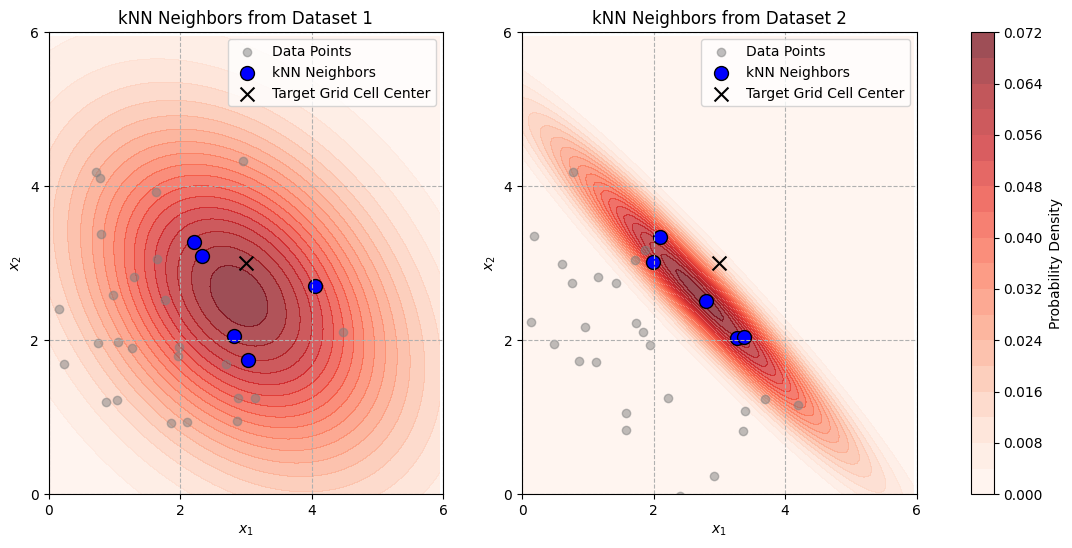
\includegraphics[scale=0.3]{./util-fig/TG-knn.png}
  \caption{kNNによるガウス分布}
  \label{fig:TG-knn}
\end{figure}
% ------------------------------------
\subsection{ガウス関数での変換と2次元ガウス特徴量(GF+TG)}
%------------------------------------
距離特徴量をガウス関数によって変換するGFと,
2次元ガウス特徴量を生成するTGを並列に入れた特徴量構成法をGF+TGとする.
%------------------------------------
\chapter{実験}
\label{chapter_4}

本研究では,\citet{caplan2015risk}が提案するRTMと同様に,
アメリカ合衆国のイリノイ州クック郡の郡庁所在地であるシカゴ市を対象領域とする.

%------------------------------------
\section{データセット}
%------------------------------------
応答変数を構成する犯罪発生地点及び,予測変数を構成する地理的リスク要因の位置情報は,
\citet{ChicagoDataPortal}のAPIを用いて緯度経度情報として取得した.

取得したデータ期間は2011年1月1日〜2014年12月31日で,
それぞれの犯罪発生地点と地理的リスク要因の位置情報は,
ともに発生時刻・記録年を基に1年単位で取得した.
表\ref{tab:2011-2014-data}に取得した全データ件数を示す.

\begin{table}
  \centering
  \caption{2011年から2014年のデータ}
  \label{tab:2011-2014-data}
  \begin{tabular}{lrrrr}
  \toprule
  カテゴリ & 2011 & 2012 & 2013 & 2014 \\
  \midrule
  強盗 & 26577 & 22783 & 17854 & 14490 \\
  \midrule
  廃墟 & 15365 & 11971 & 8363 & 5446 \\
  放置車両 & 19907 & 17390 & 16077 & 20358 \\
  路地灯消灯 & 46697 & 19944 & 15177 & 21684 \\
  街灯消灯 & 33895 & 30893 & 22650 & 64857 \\
  学校 & 674 & 681 & 672 & 680 \\
  差し押さえ物件 & 16680 & 16120 & 11131 & 7511 \\
  落書き除去 & 136873 & 109908 & 137058 & 124721 \\
  不衛生な場所 & 17888 & 19088 & 18029 & 18997 \\
  \midrule
  暴行 & 60306 & 58998 & 53887 & 49230 \\
  器物損壊 & 37234 & 35771 & 30779 & 27637 \\
  窃盗 & 74770 & 75170 & 71270 & 61127 \\
  性的暴行 & 1402 & 1347 & 1197 & 1216 \\
  売春 & 2424 & 2200 & 1652 & 1608 \\
  賭博 & 736 & 724 & 596 & 393 \\
  酒類法違反 & 619 & 573 & 464 & 394 \\
  武器違反 & 3879 & 3904 & 3240 & 3099 \\
  誘拐 & 266 & 234 & 242 & 217 \\
  公務執行妨害 & 1041 & 1227 & 1277 & 1393 \\
  傷害 & 20343 & 19848 & 17920 & 16830 \\
  殺人 & 437 & 515 & 431 & 428 \\
  性犯罪 & 1053 & 1035 & 1004 & 909 \\
  詐欺行為 & 12329 & 13239 & 13215 & 14788 \\
  自動車盗難 & 19353 & 16450 & 12552 & 9846 \\
  薬物犯罪 & 38527 & 35417 & 34057 & 28836 \\
  放火 & 504 & 469 & 363 & 394 \\
  脅迫 & 171 & 156 & 133 & 114 \\
  児童関連犯罪 & 2281 & 2190 & 2319 & 2304 \\
  不法侵入 & 8634 & 8197 & 8122 & 7500 \\
  ストーカー行為 & 181 & 206 & 153 & 140 \\
  治安妨害 & 3089 & 3001 & 3131 & 2896 \\
  その他の犯罪 & 20134 & 17471 & 17979 & 16902 \\
  \bottomrule
  \end{tabular}
  \end{table}
  
%------------------------------------
\section{RTMの構成}
%------------------------------------
分析にあたっては,対象地域に130m×130mのグリッドセルを設定し,
各グリッドセルでの犯罪発生リスクを予測する.
応答変数は各グリッドセルで発生した犯罪件数,予測変数は地理的リスク要因から生成した特徴量である.

%------------------------------------
\subsection{データの前処理}
%------------------------------------
取得したデータは,地理的座標系に基づいており,緯度経度情報として提供されているが,
本研究では距離計算や空間分析を正確に行うため,PythonのGeoPandasライブラリを使用し,
メートル単位での解析が可能な平面直角座標系(EPSG:26971)に変換した.
また,データ品質を保証するため,明らかに誤った位置情報(NaN,0,etc.)と,
シカゴ市領域外の位置情報は事前に除外した.

本研究では,応答変数の分布をyeo-jhonson変換\citep{weisberg2001yeo}により正規分布に近づける.
実装にはsklearn.preprocessing.PowerTransformerを用いた.
また応答変数と予測変数の標準化も実行した.

%------------------------------------
\subsection{パラメータ探索}
%------------------------------------
本研究では,前処理したデータに対して,Lasso回帰を実行することによって変数選択した.
また最適な正則化パラメータは,20foldの交差検証で探索した.
実装には,sklearnのLassoCVを用いた.


%------------------------------------
\subsection{犯罪発生リスク算出}
%------------------------------------
モデルの出力値に対して,前処理で実行したyeo-jhonson変換の逆変換を行って,
予測値の分布を元の犯罪の分布に近づけた.モデルの予測値は連続値であるため,
精度評価やリスクマップ表示の際には,予測値をそれぞれを適切な基準で離散化する.

%------------------------------------
\section{評価方法}
%------------------------------------
モデルが予測した犯罪発生リスクを,
高リスク($平均+1標準偏差以上$)と低リスク($平均+1標準偏差未満$)にカテゴリー化する.
各手法の予測精度は,犯罪予測の文脈で一般的な
的中率とPAI(Predictive Accuracy Index)とROC曲線・AUCの3つの指標で年単位の評価を行う.

的中率とは,予測モデルが「高リスク」と特定したエリアの中で、実際に犯罪が発生した割合である.
(\ref{hitrate})式に的中率の計算式を示す.

\begin{equation}\label{hitrate}
  的中率=\frac{高リスクと予測されたエリア内で実際に発生した犯罪の数}{実際に発生した犯罪の総数}
\end{equation}

的中率のみの評価では,高リスクエリアが広がりすぎて,実用上の有用性が下がる可能性があるため,
これに加えて\citet{chainey2008utility}が考案したPAIを評価に用いる.

PAIとは,高リスクエリア内で発生した犯罪の割合を、そのエリアの全体に占める面積割合で割った値である.
PAIが高いほど、モデルの予測精度が高いとされる.
(\ref{pai})式に的中率の計算式を示す.

\begin{equation}\label{pai}
  PAI=\frac{的中率}
  {\frac{高リスクエリアの面積}{全エリアの面積}}
\end{equation}

ROC(Receiver Operating Characteristic)曲線とは,
機械学習モデルの分類性能を評価するための代表的な手法の1つである.
ROC曲線は,分類モデルの予測スコアに対して異なる閾値を設定し,
それに応じた真陽性率(True Positive Rate, TPR)と
偽陽性率(False Positive Rate, FPR)をプロットすることで得られる.
曲線の下の面積がAUC(Area Under the Curve)と呼ばれ,
モデルの識別能力を定量的に表す指標として用いられる.
AUCは0.5から1.0の範囲を取り,この値が大きいほどモデルの分類性能が優れていることを意味する.
%------------------------------------
\section{時系列に配慮しない方法}
%------------------------------------
2011〜2013年を学習データ,2014年をテストデータとして,
学習データの時系列は配慮せずにモデルを学習させて,6種のモデルの予測精度を比較する.

%------------------------------------
\subsection{実験条件}
%------------------------------------

応答変数は,各グリッドセル内で発生した強盗犯罪件数である.
予測変数として用いた地理的リスク要因は,
廃屋,放置車両,路地灯消灯,街灯消灯,学校,差し押さえ物件,落書き除去,不衛生な場所
の8つである.

なお,従来手法による離散型特徴量の構成に用いた,特定の距離とバンド幅とは271m,591m,779m,1003mである.
これらの距離はシカゴ市の2ブロック,4ブロック,6ブロック,8ブロックに相当する.

また,NEの$\gamma$には$1,2,3$を代入し,1つの地理的リスク要因の距離特徴量から,3つの特徴量を生成した.
LDとGFにおける$\sigma$には,
$3$を底とした対数スケールで$1,2,5,12,30,71,168,395,930,2187$の10種類の値を代入して,
1つの地理的リスク要因の距離特徴量から,ラプラス分布関数で変換した5つの特徴量を生成した.
TGにおける$K$は,$5, 10, 15, 20, 25$の5つの値を代入して,
1つの地理的リスク要因の距離特徴量から,5つの特徴量を生成した.

%------------------------------------
\subsection{結果}
\label{non-crime-no-timeseries-result}
%------------------------------------
RTMが出力した連続値の犯罪発生リスクを,
平均未満,平均以上1標準偏差未満,1標準偏差以上2標準偏差未満,2標準偏差以上の4カテゴリーに分割した.
4カテゴリーの混同行列作成し,各グリッドセルの犯罪発生リスクをリスクマップとして地図上にを図示した.

また,RTMが出力した高リスクと低リスクの2カテゴリーから混同行列を作成し,
False Positive(FP)・False Negative(FN)のグリッドセルを地図上に図示する.

2011年〜2013年でモデルを学習し,2014年で評価した結果を示す.
2014年に実際に起った強盗犯罪の発生地点とそれに基づいた実際のリスクマップを
図\ref{fig:non-crime-no-timeseries-actual-risk}に示す.

DFによる予測結果を図\ref{fig:non-crime-no-timeseries-df-risk}に,
CFによる予測結果を図\ref{fig:non-crime-no-timeseries-cf-risk}に示す.
実際のリスクマップと比べて,離散型特徴量によるリスクマップでは高い空間相関を持つが,
連続型特徴量によるリスクマップは空間相関が削減された.

NEによるリスクマップを図\ref{fig:non-crime-no-timeseries-ne-risk}に,
LDによるリスクマップを図\ref{fig:non-crime-no-timeseries-ld-risk}に,
GFによるリスクマップを図\ref{fig:non-crime-no-timeseries-gf-risk}に,
TGによるリスクマップを図\ref{fig:non-crime-no-timeseries-tg-risk}に,
GF+TGによるリスクマップを図\ref{fig:non-crime-no-timeseries-gf-tg-risk}に示した.


また,
4カテゴリーの混同行列を図\ref{fig:non-crime-no-timeseries-4cm}に,
2カテゴリーの混同行列を図\ref{fig:non-crime-no-timeseries-2cm}に,
各モデルによるFP・FNのグリッドセルを
図\ref{fig:non-crime-no-timeseries-df-fnp}から
図\ref{fig:non-crime-no-timeseries-gf-tg-fnp}に示した.

%------------------------------------------
% risk map
%------------------------------------------
\begin{figure}
  \centering % 図を中央寄せにする
  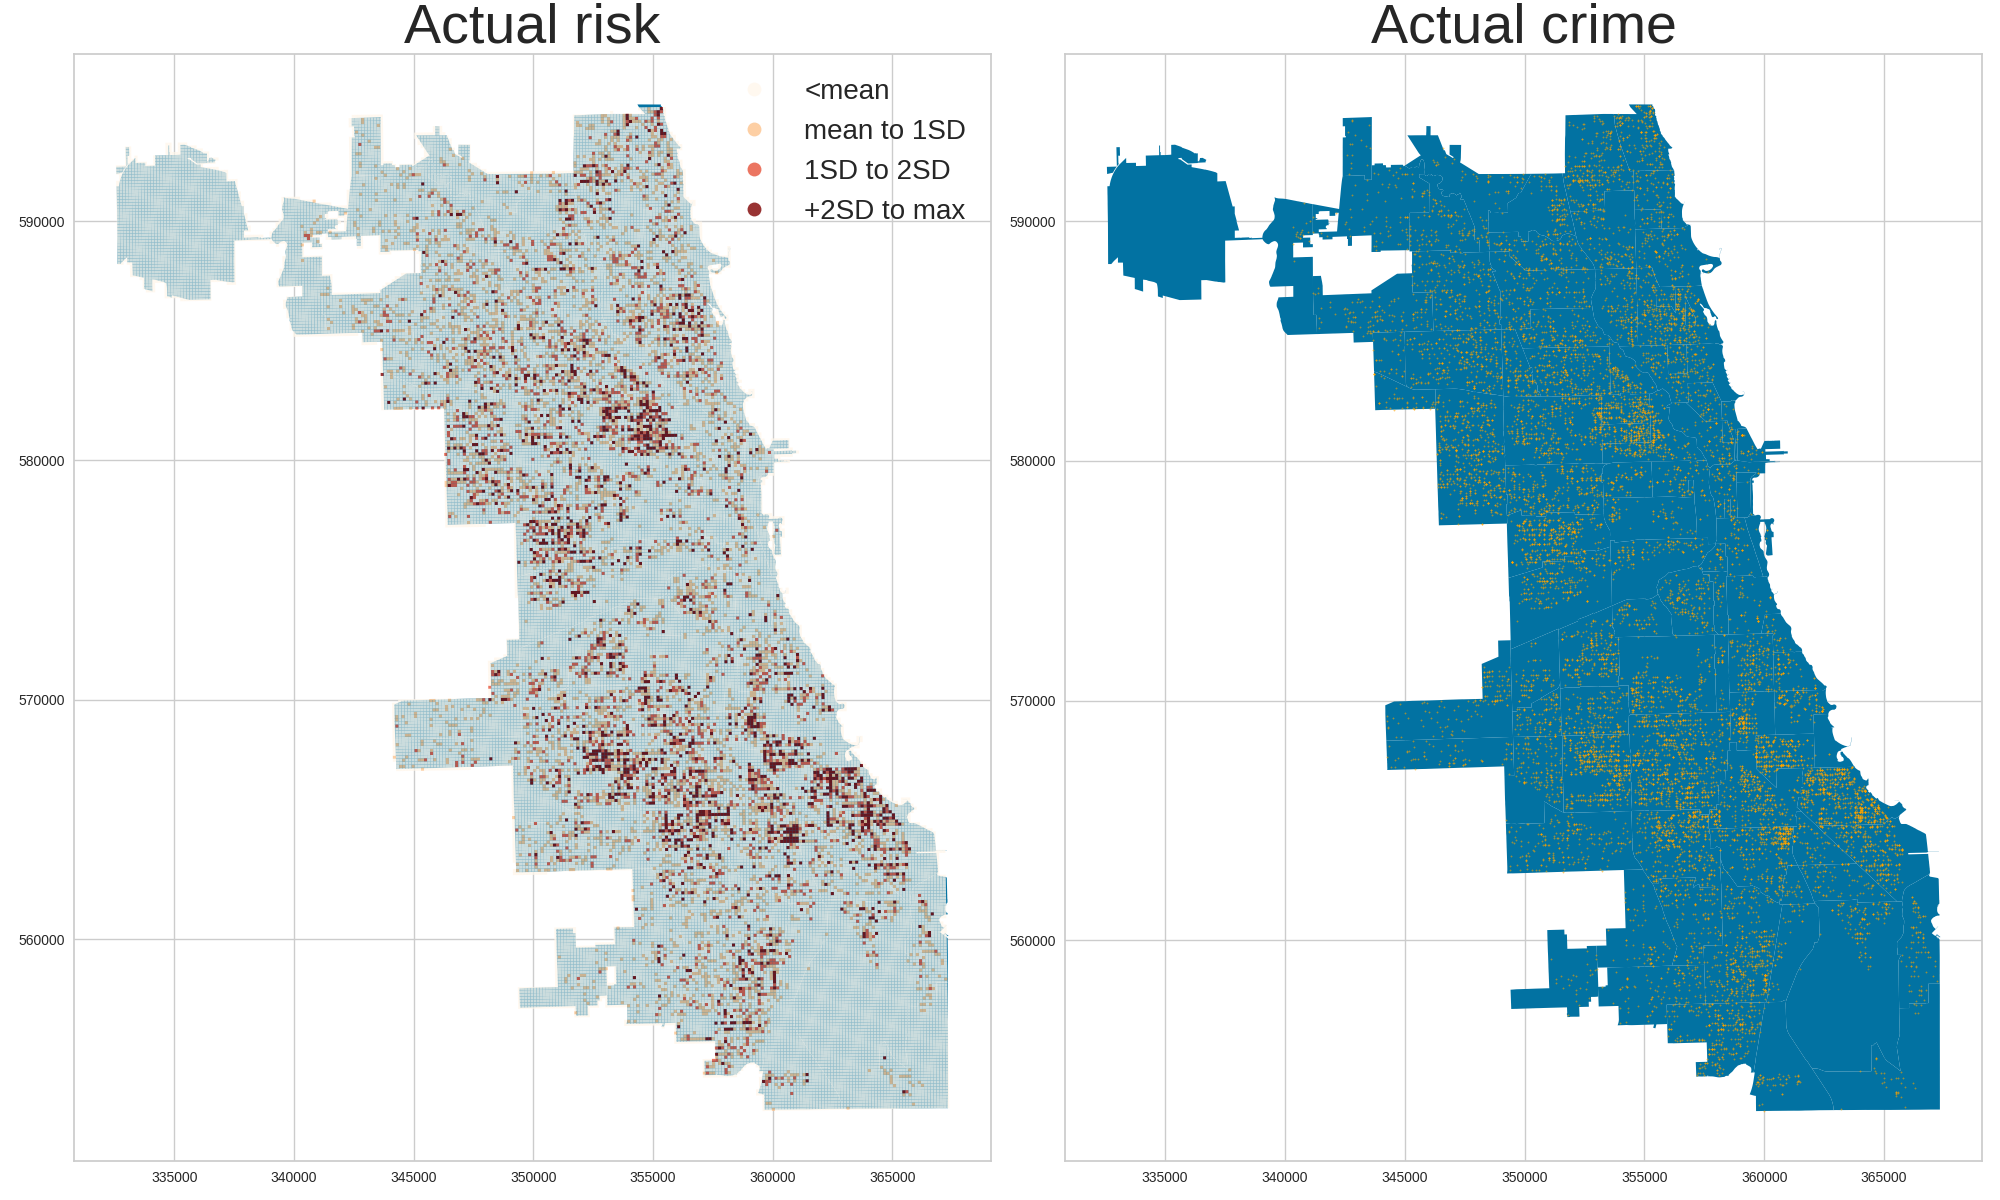
\includegraphics[scale=0.25]{./non-crime-no-timeseries-fig/actual_risk_point_map.png}
  \caption{左:実際のリスクマップ 右:実際の強盗犯罪発生地点}
  \label{fig:non-crime-no-timeseries-actual-risk}
\end{figure}

\begin{figure}
  \centering % 図を中央寄せにする
  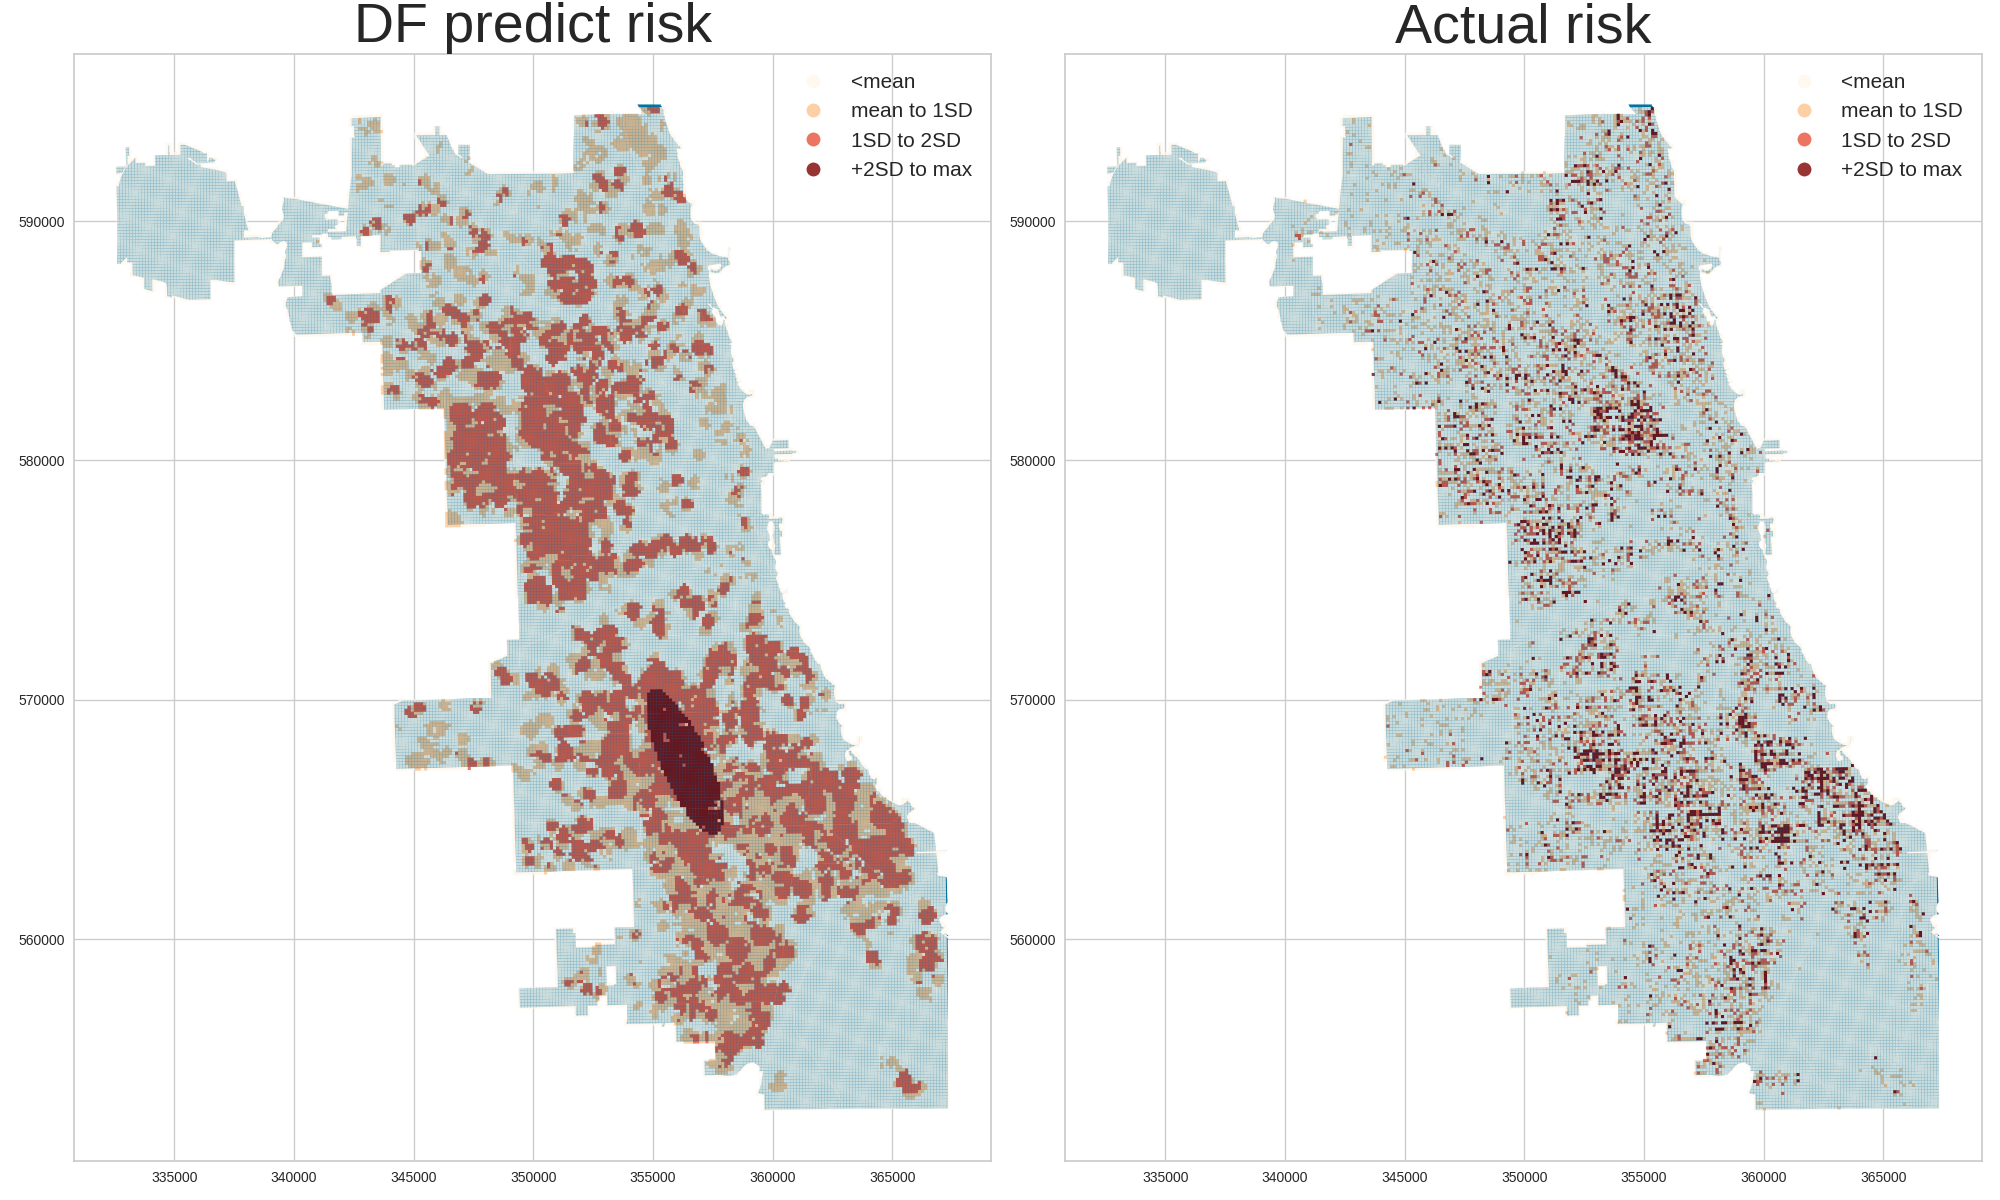
\includegraphics[scale=0.25]{./non-crime-no-timeseries-fig/DF_riskmap.png}
  \caption{左:DFによるリスクマップ 右:実際のリスクマップ}
  \label{fig:non-crime-no-timeseries-df-risk}
\end{figure}

\begin{figure}
  \centering % 図を中央寄せにする
  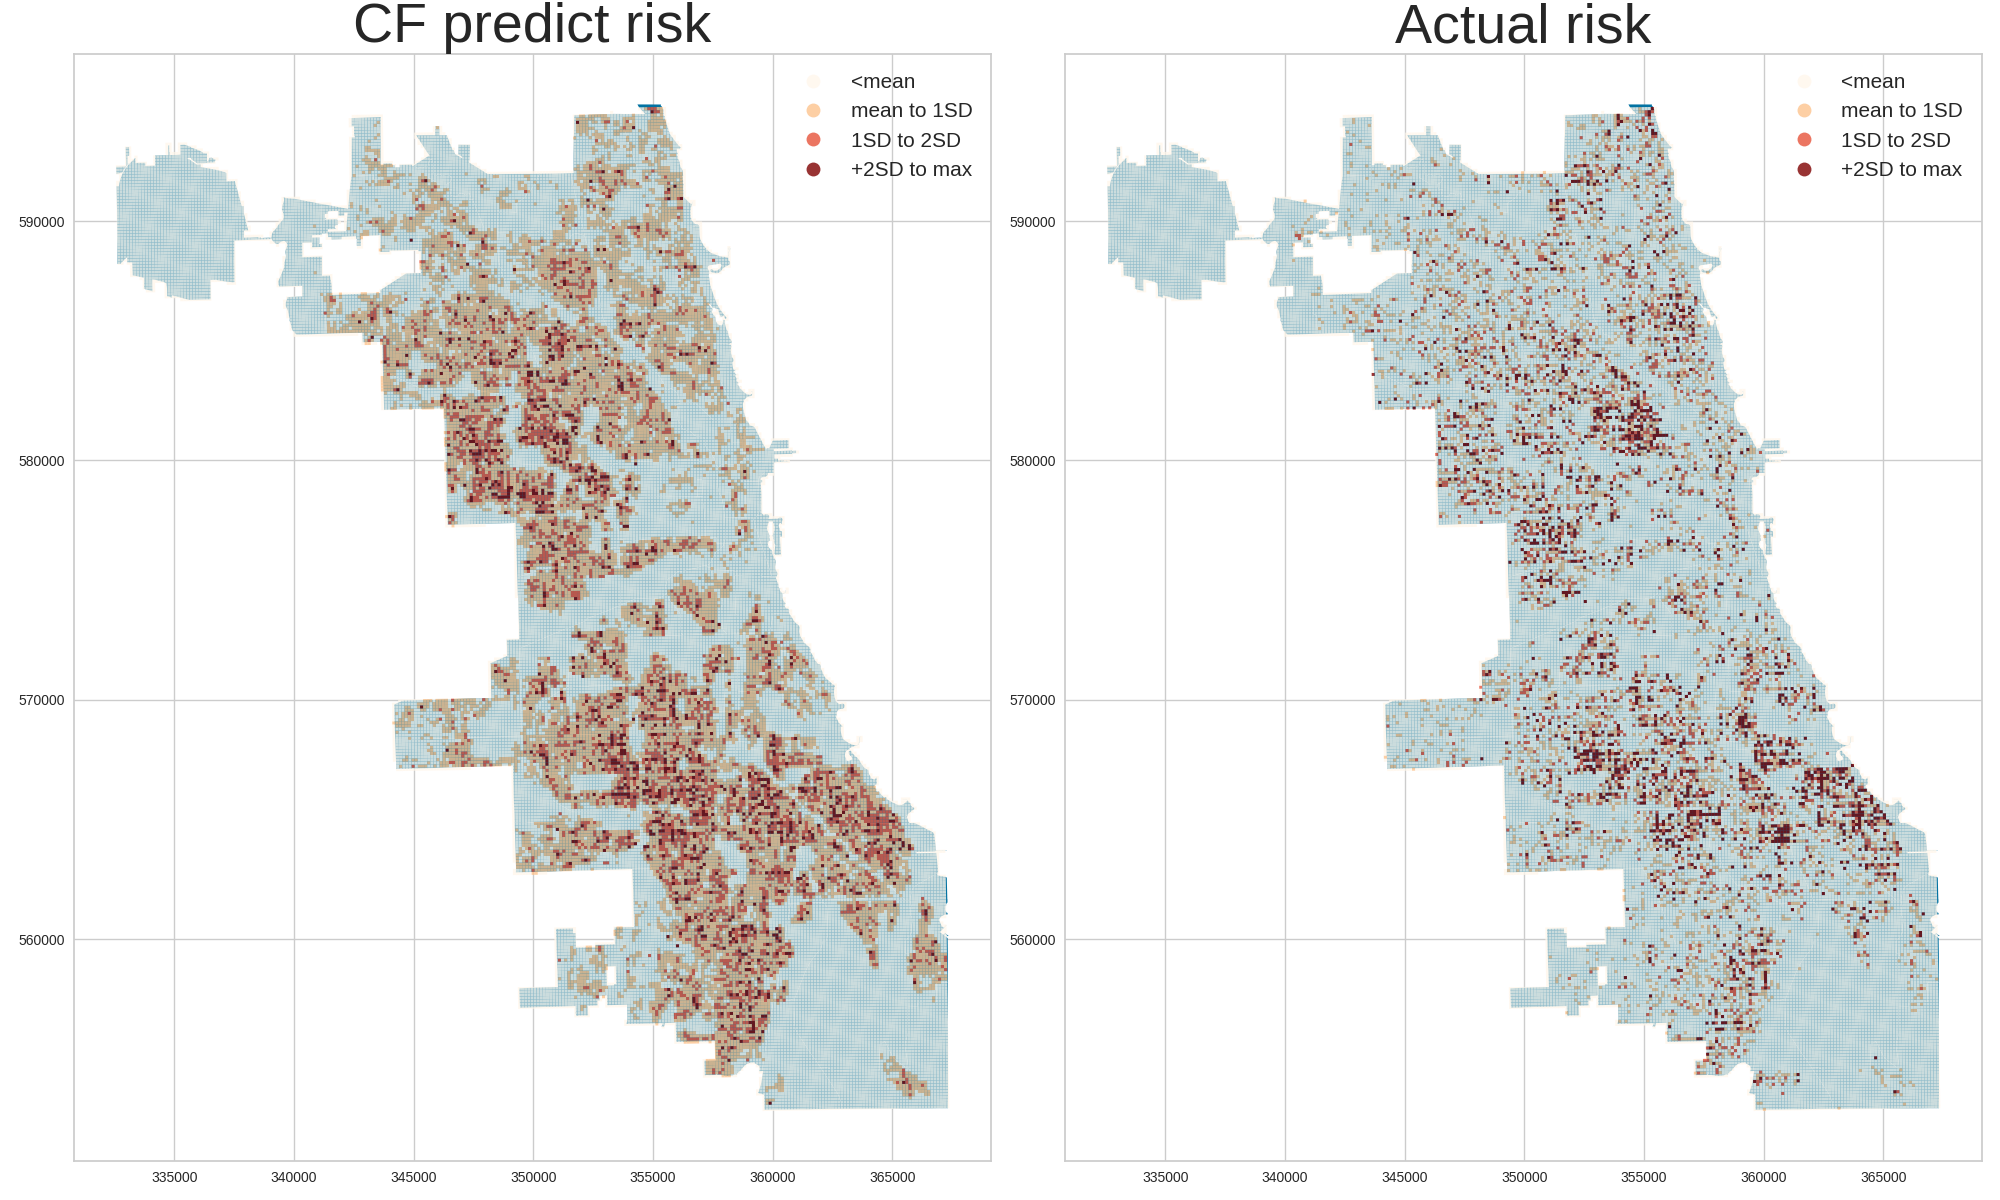
\includegraphics[scale=0.25]{./non-crime-no-timeseries-fig/CF_riskmap.png}
  \caption{左:CFによるリスクマップ 右:実際のリスクマップ}
  \label{fig:non-crime-no-timeseries-cf-risk}
\end{figure}

\begin{figure}
  \centering % 図を中央寄せにする
  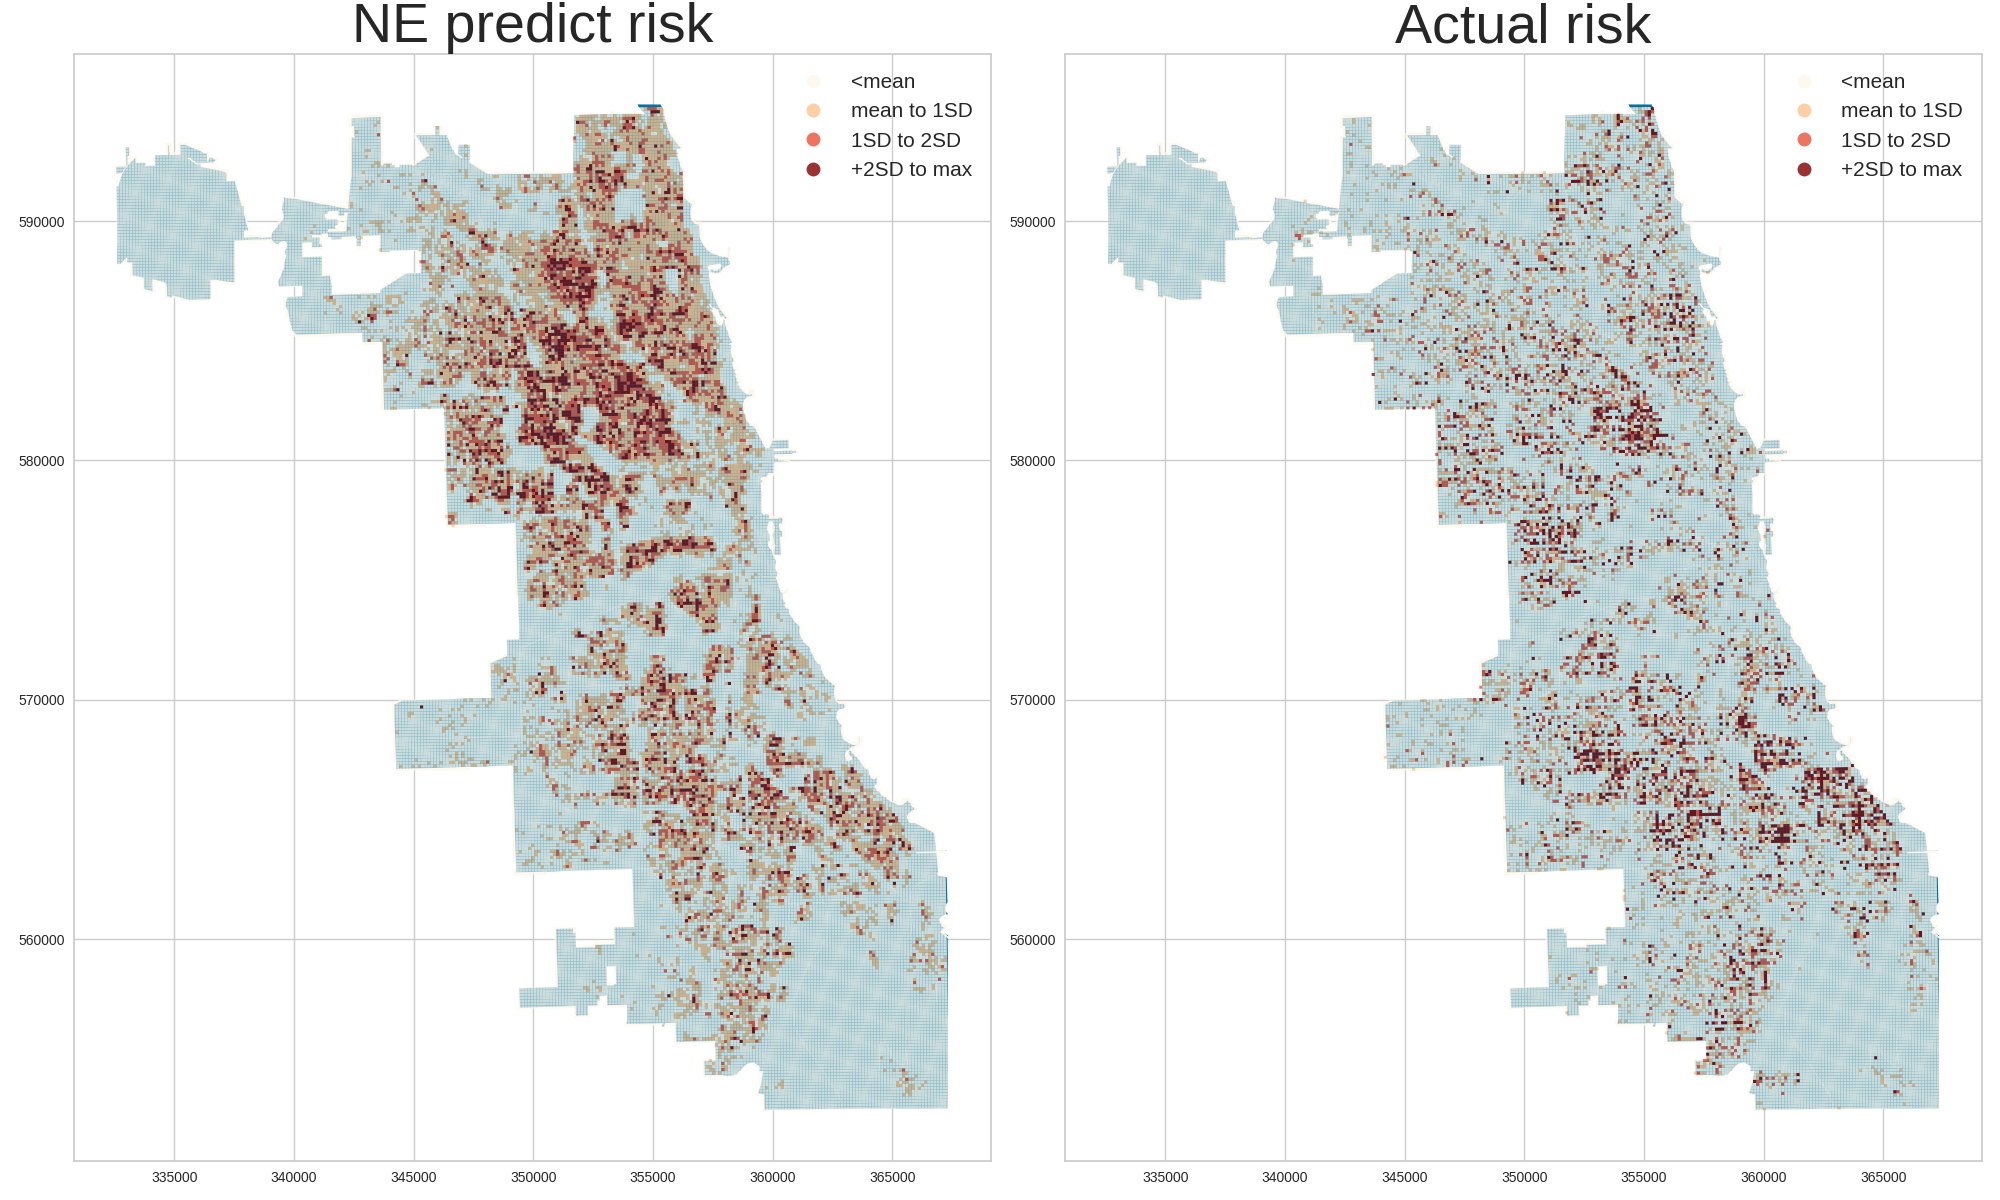
\includegraphics[scale=0.25]{./non-crime-no-timeseries-fig/NE_riskmap.png}
  \caption{左:NEによるリスクマップ 右:実際のリスクマップ}
  \label{fig:non-crime-no-timeseries-ne-risk}
\end{figure}

\begin{figure}
  \centering % 図を中央寄せにする
  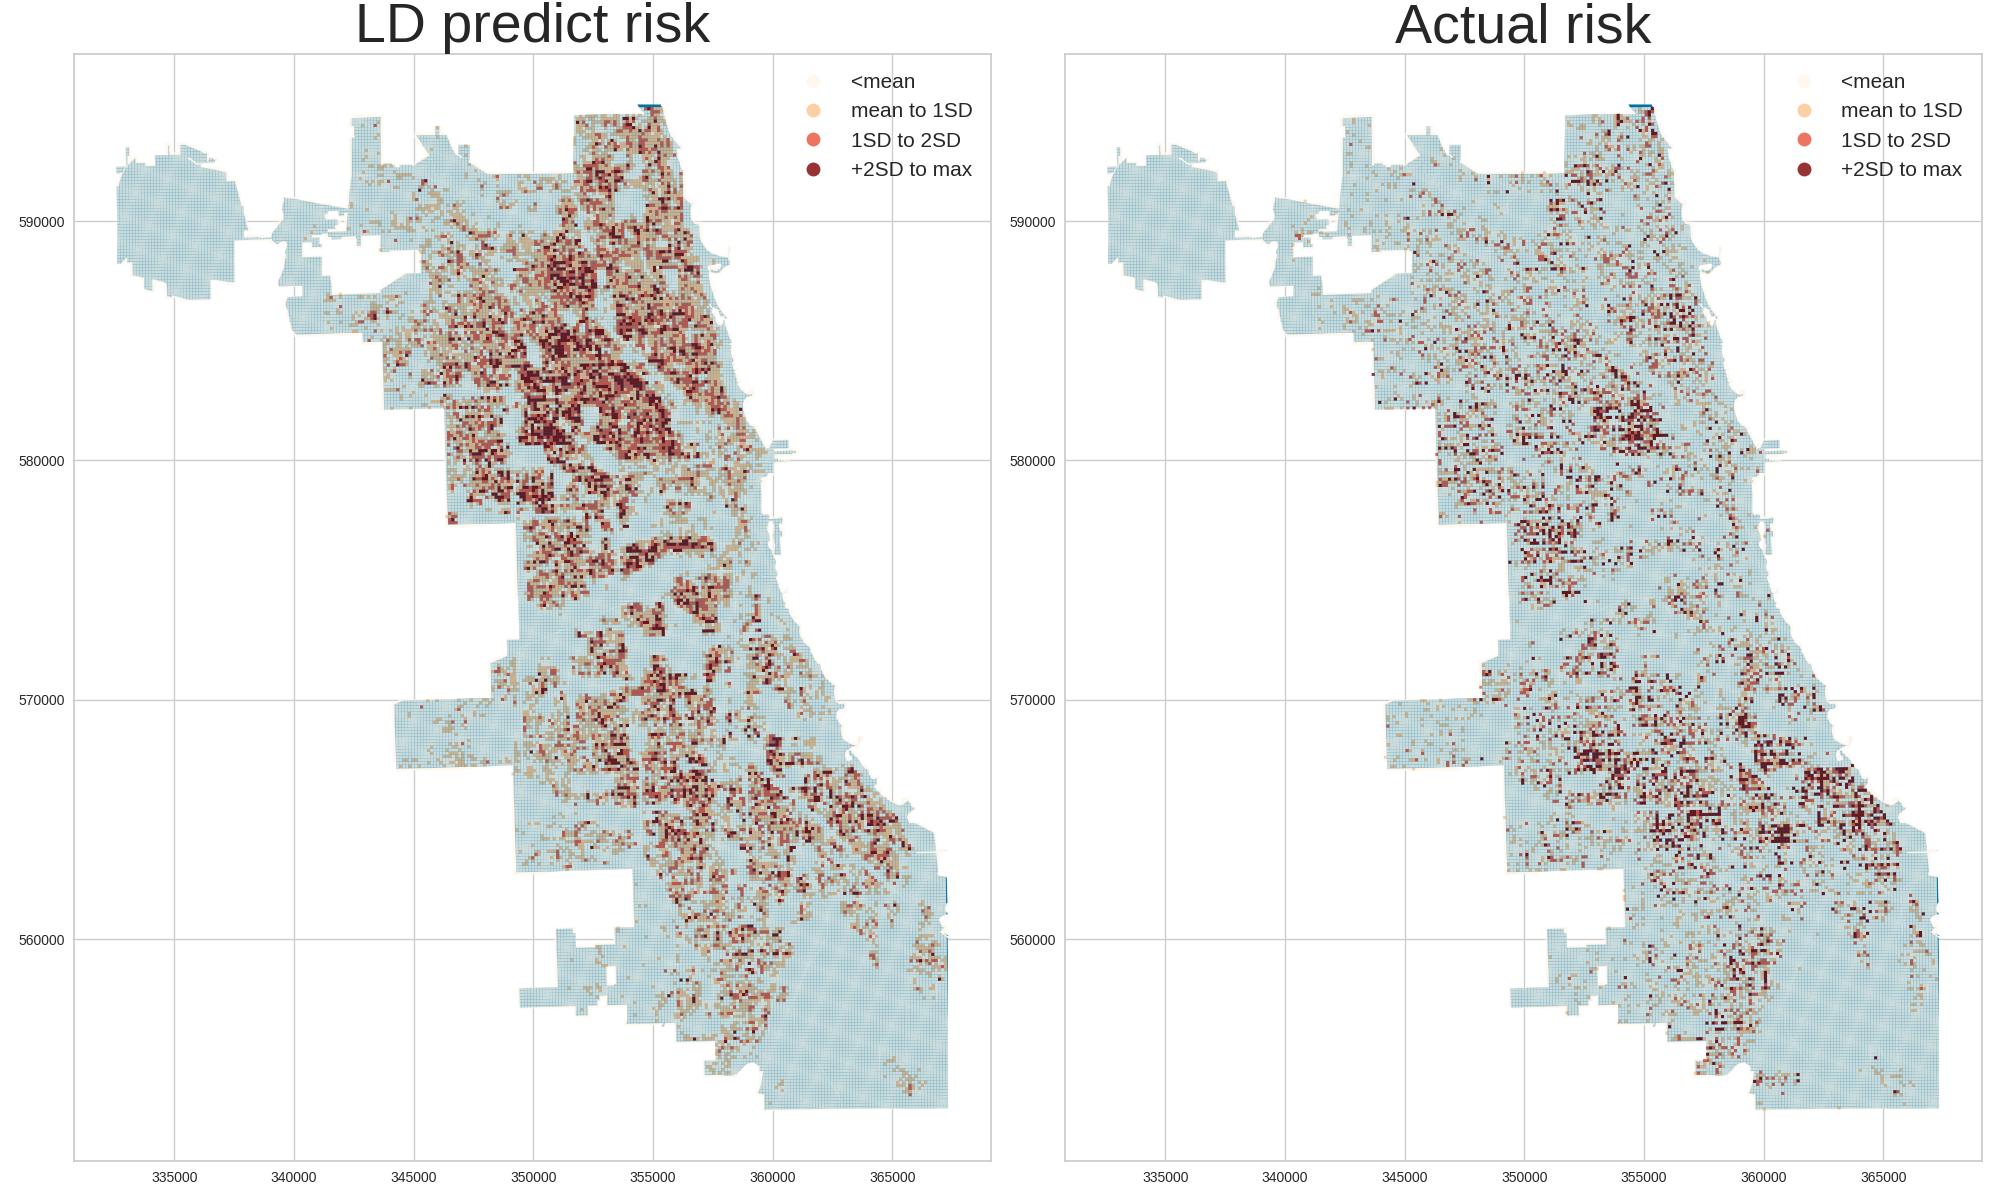
\includegraphics[scale=0.25]{./non-crime-no-timeseries-fig/LD_riskmap.png}
  \caption{左:LDによるリスクマップ 右:実際のリスクマップ}
  \label{fig:non-crime-no-timeseries-ld-risk}
\end{figure}

\begin{figure}
  \centering % 図を中央寄せにする
  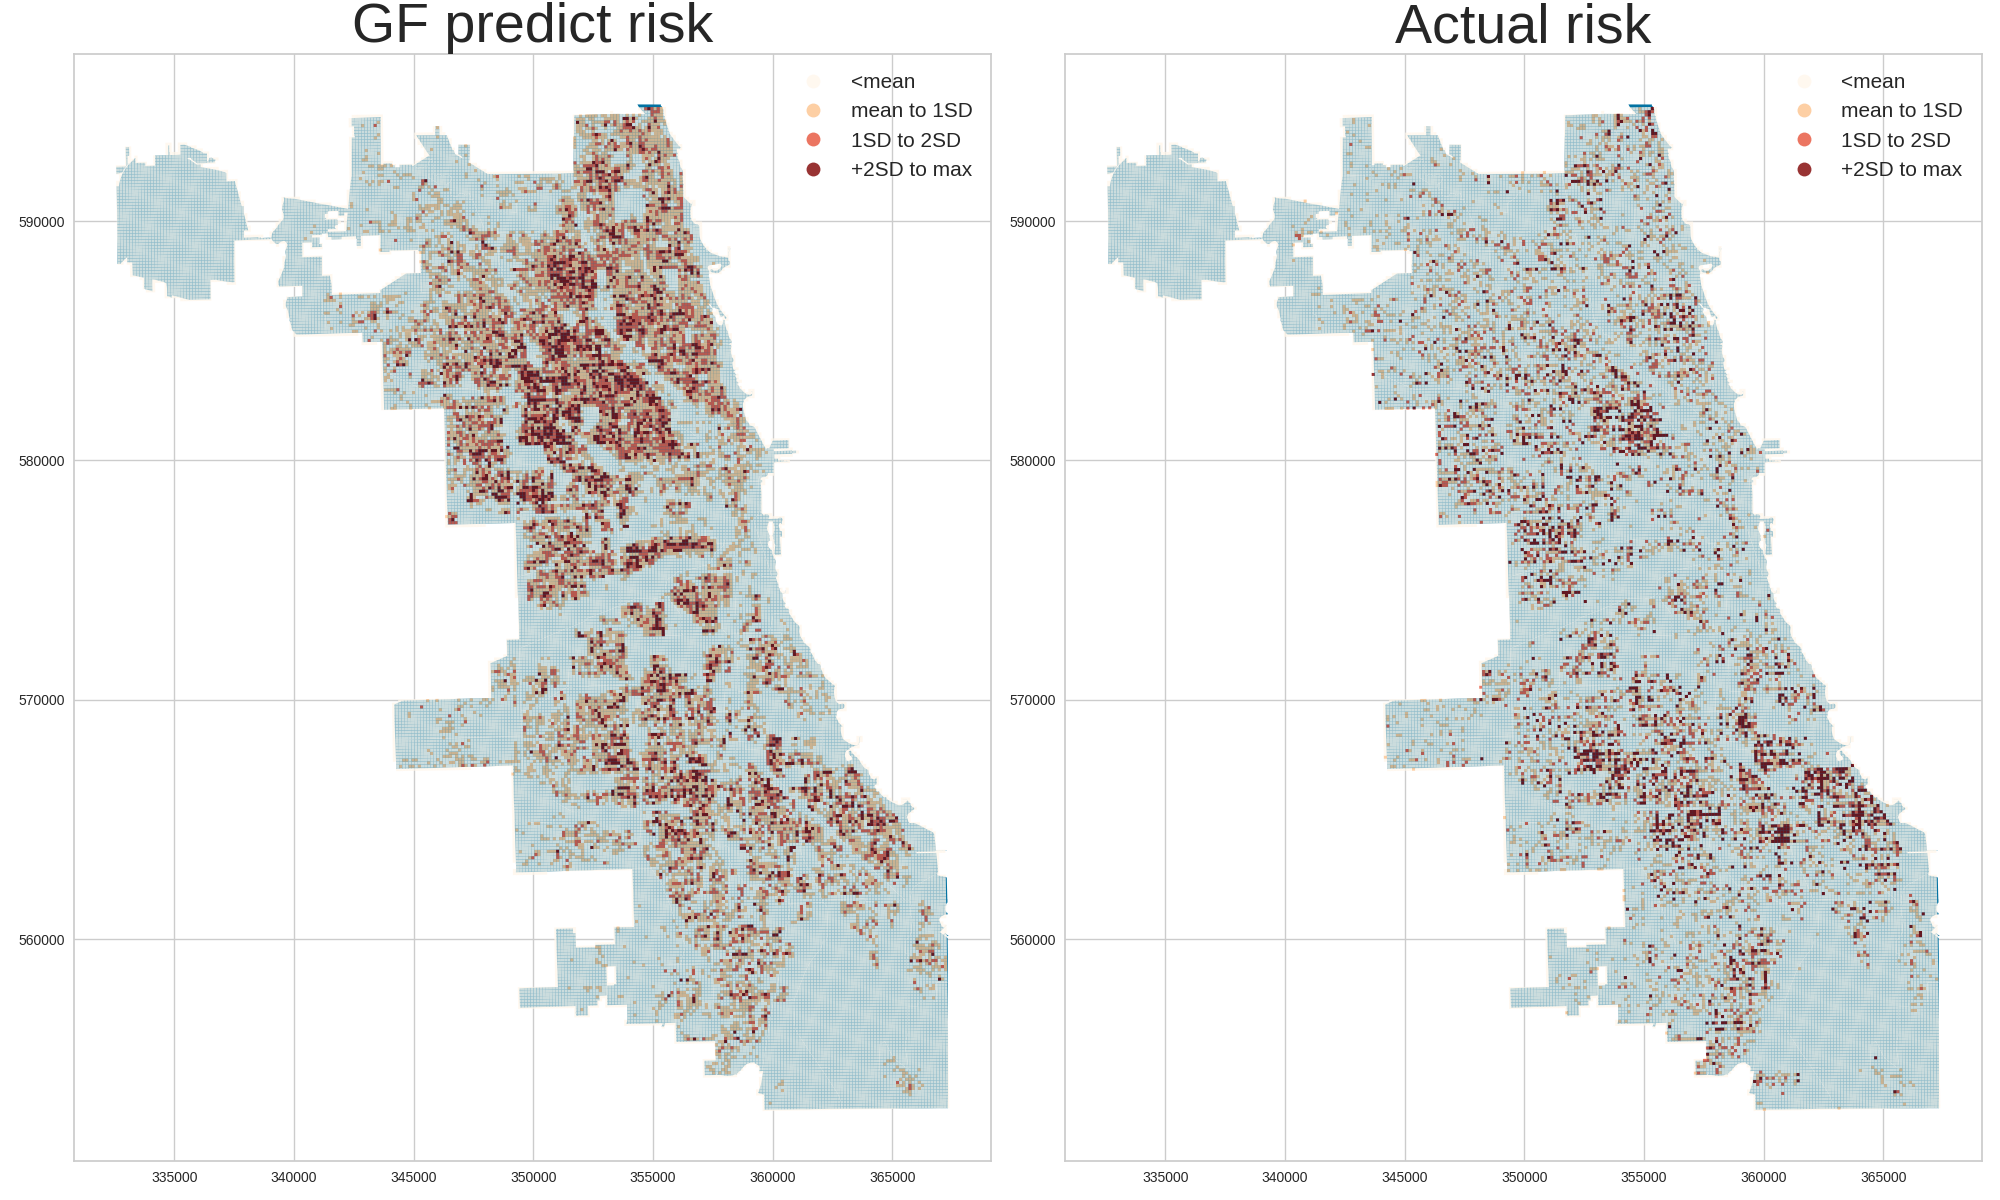
\includegraphics[scale=0.25]{./non-crime-no-timeseries-fig/GF_riskmap.png}
  \caption{左:GFによるリスクマップ 右:実際のリスクマップ}
  \label{fig:non-crime-no-timeseries-gf-risk}
\end{figure}

\begin{figure}
  \centering % 図を中央寄せにする
  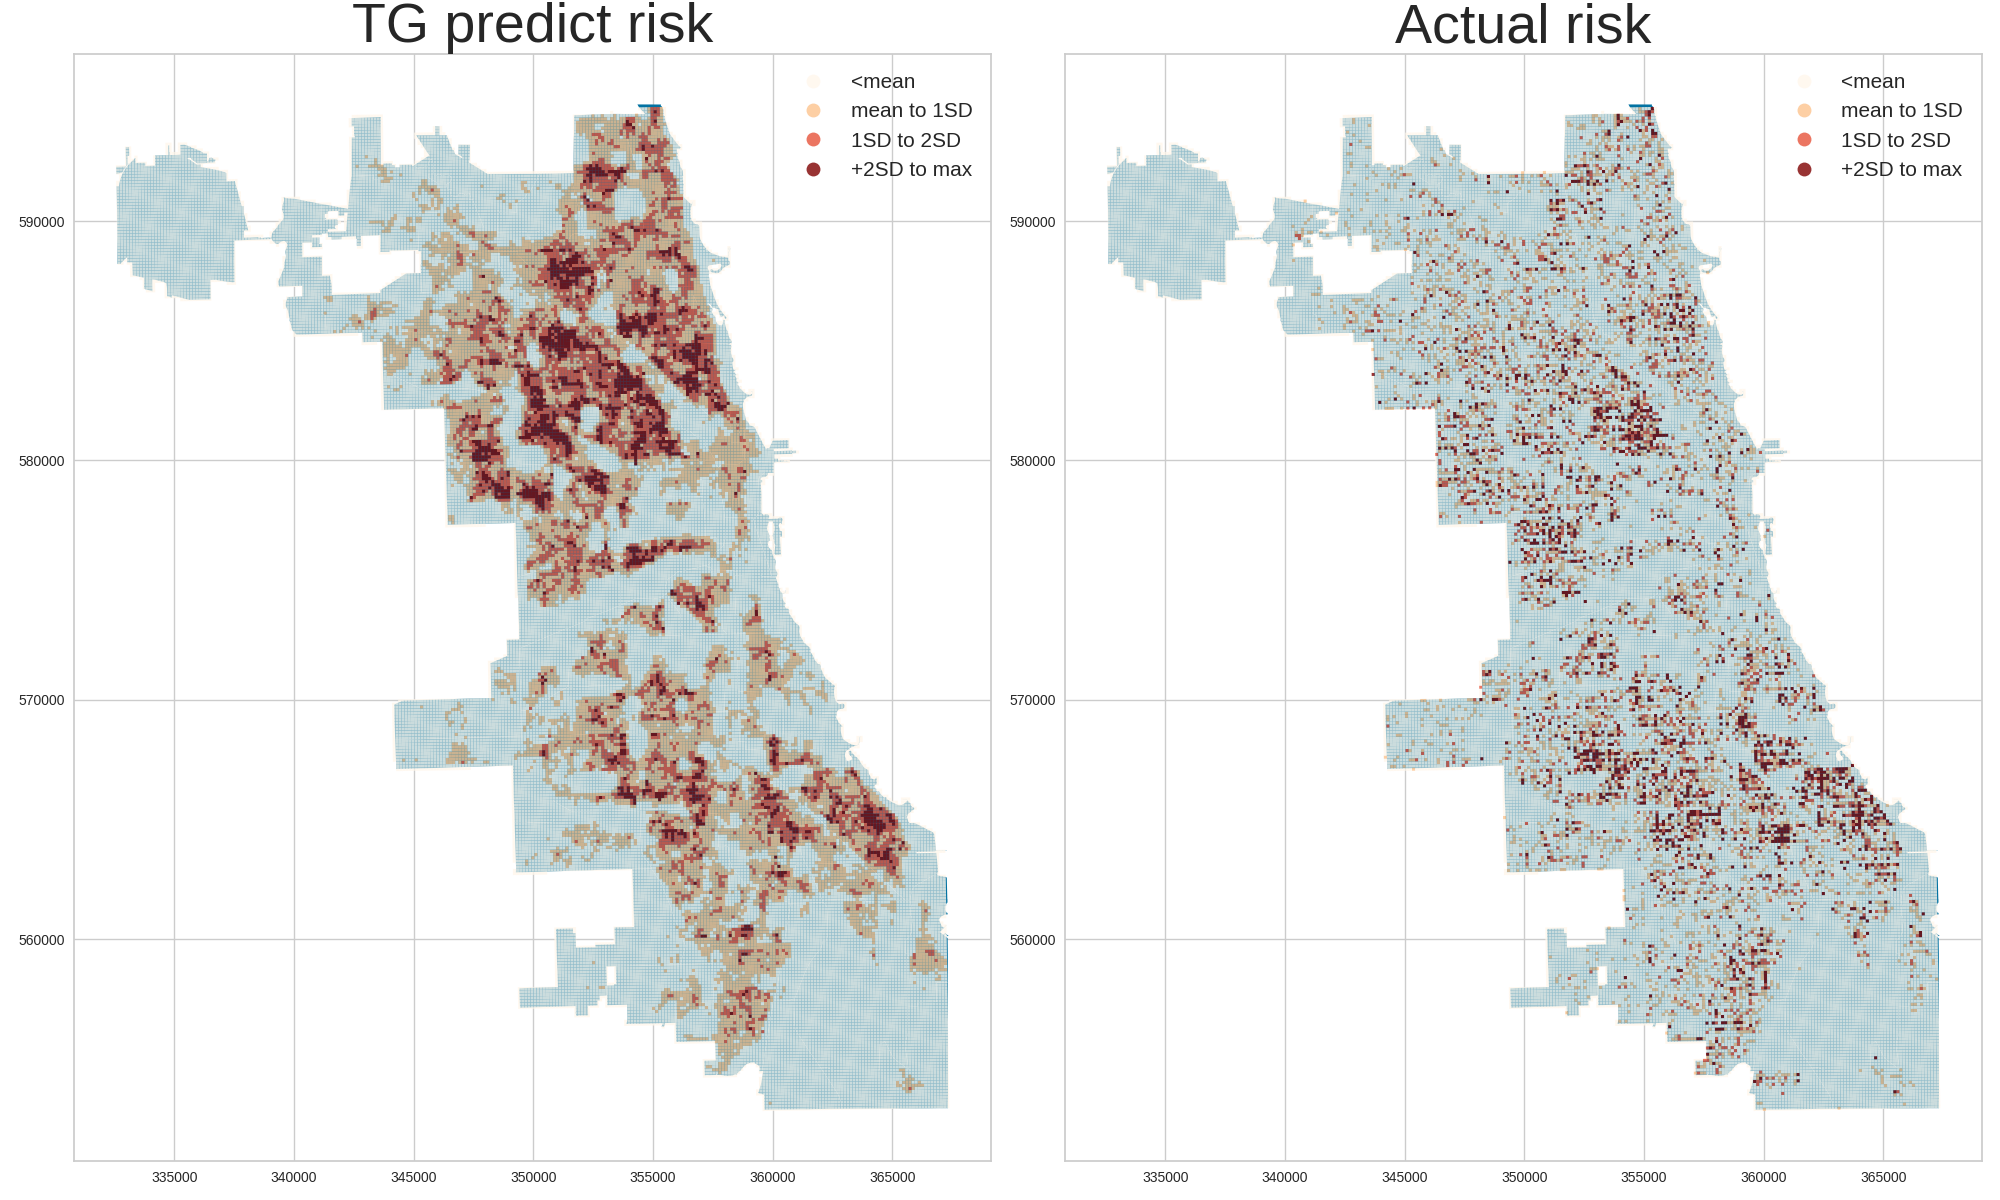
\includegraphics[scale=0.25]{./non-crime-no-timeseries-fig/TG_riskmap.png}
  \caption{左:TGによるリスクマップ 右:実際のリスクマップ}
  \label{fig:non-crime-no-timeseries-tg-risk}
\end{figure}

\begin{figure}
  \centering % 図を中央寄せにする
  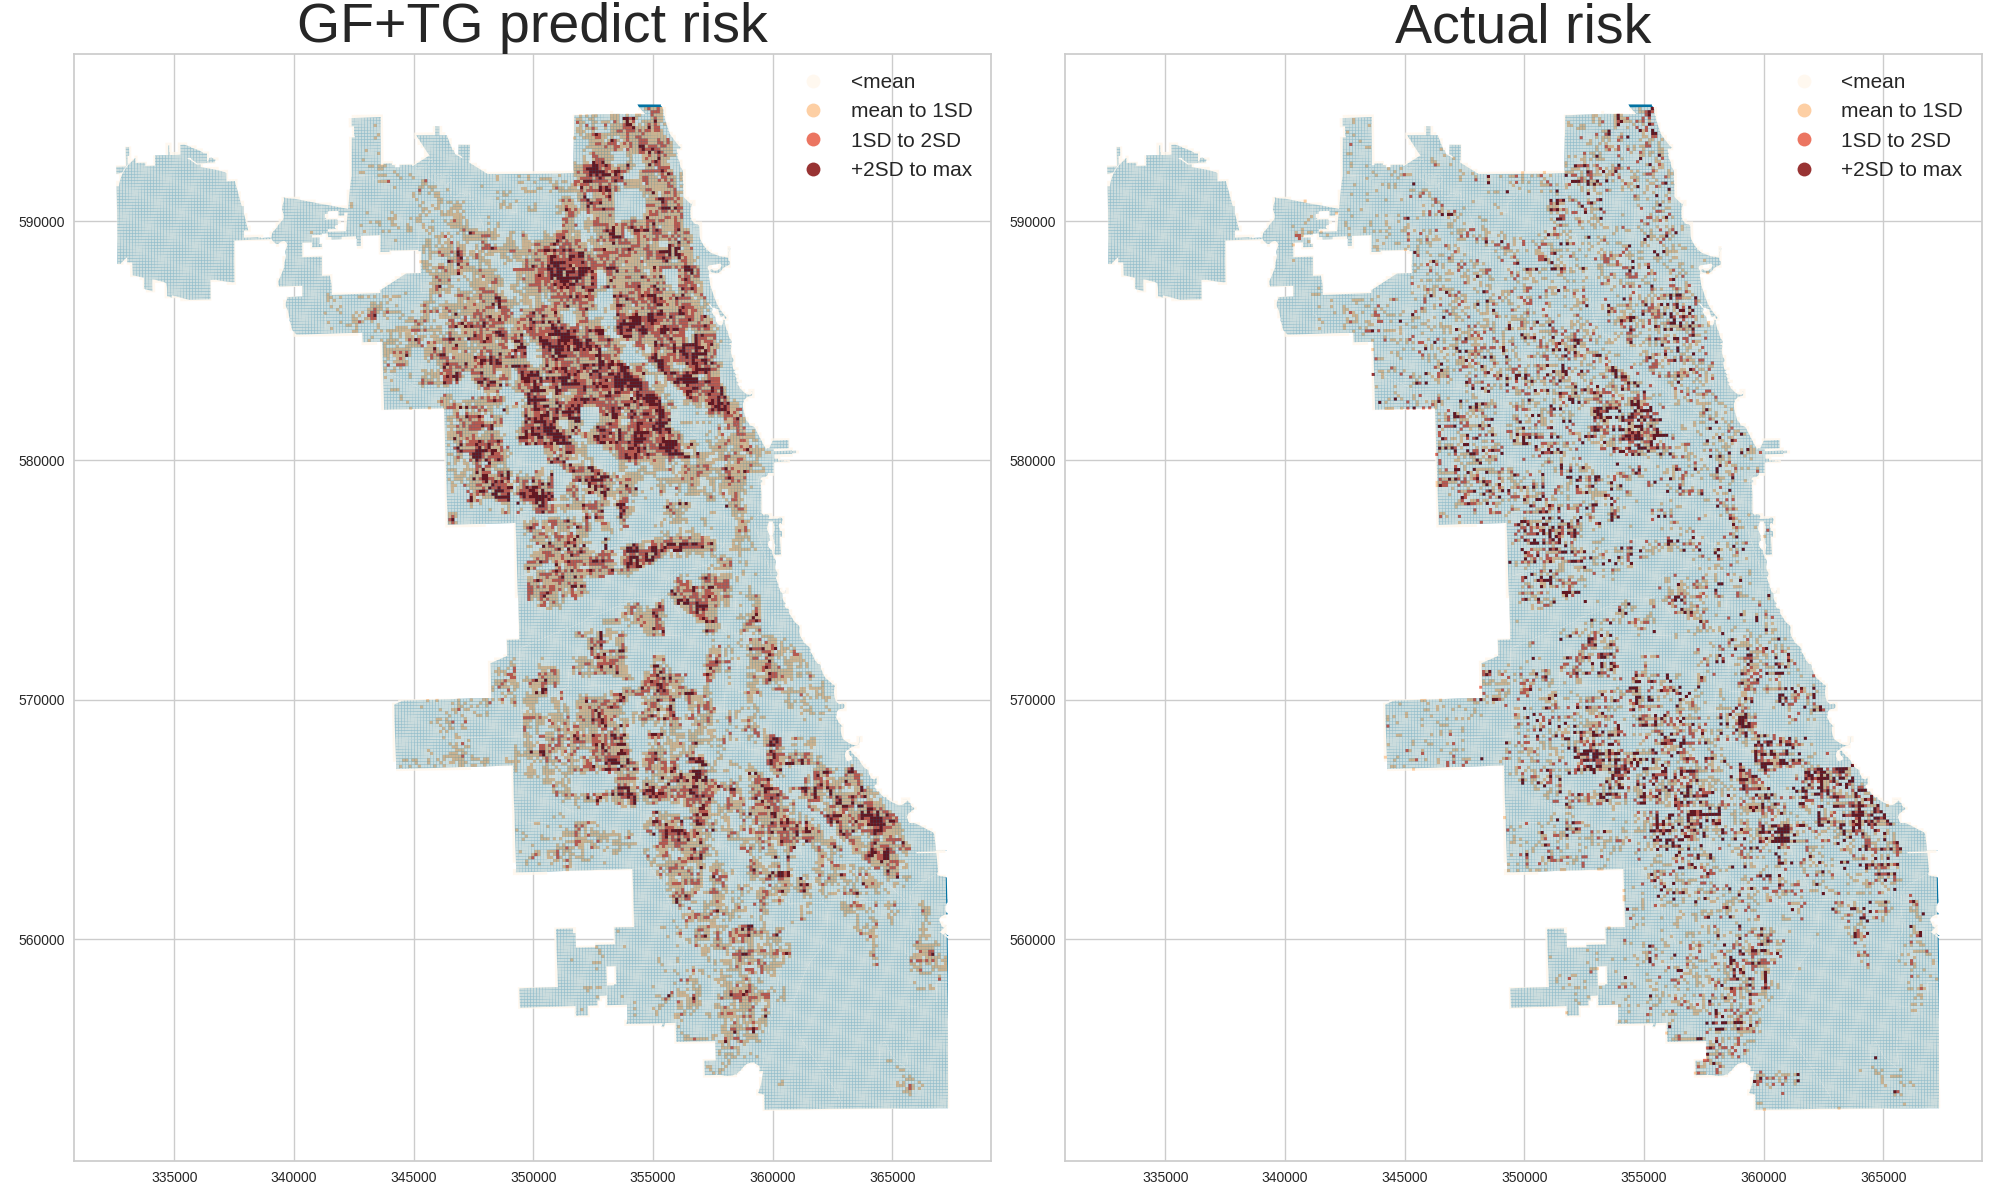
\includegraphics[scale=0.25]{./non-crime-no-timeseries-fig/GF+TG_riskmap.png}
  \caption{左:FG+TGによるリスクマップ 右:実際のリスクマップ}
  \label{fig:non-crime-no-timeseries-gf-tg-risk}
\end{figure}
%------------------------------------------
% confusion matrix
%------------------------------------------
\begin{figure}
  \centering % 図を中央寄せにする
  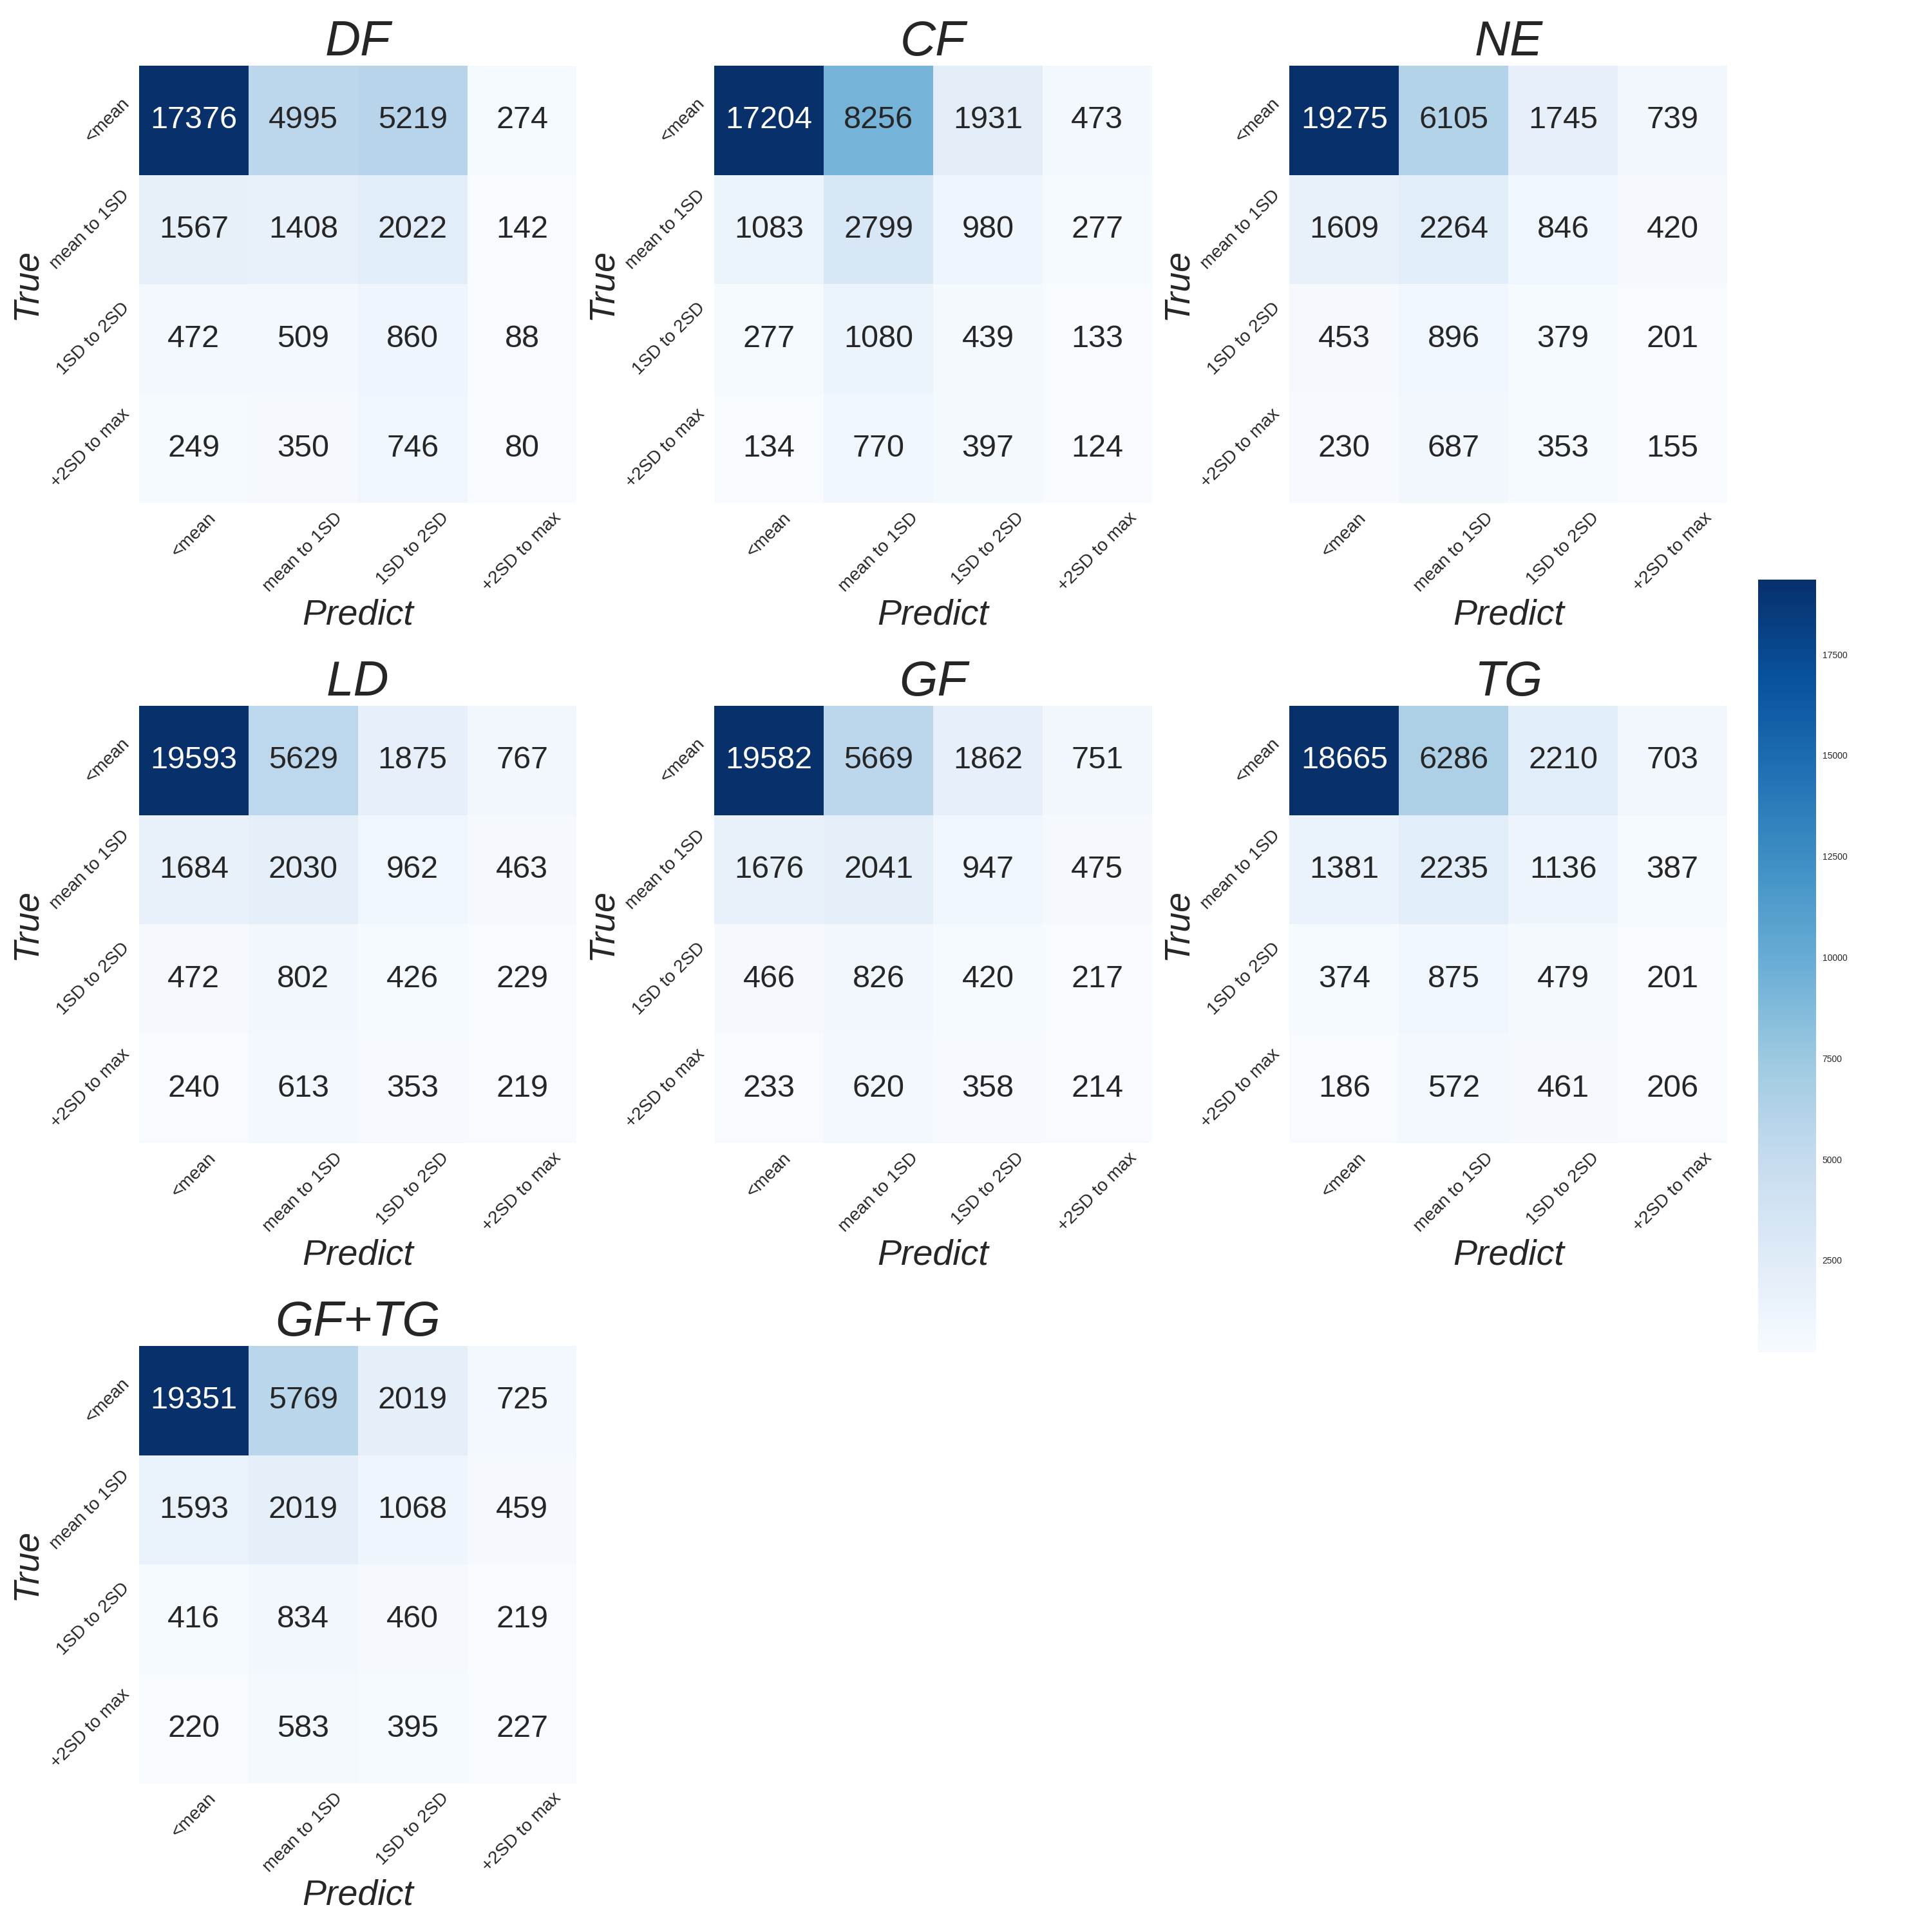
\includegraphics[scale=0.16]{./non-crime-no-timeseries-fig/non_crime_no_timeseries_four_cm.png}
  \caption{4カテゴリーの混同行列}
  \label{fig:non-crime-no-timeseries-4cm}
\end{figure}

\begin{figure}
  \centering % 図を中央寄せにする
  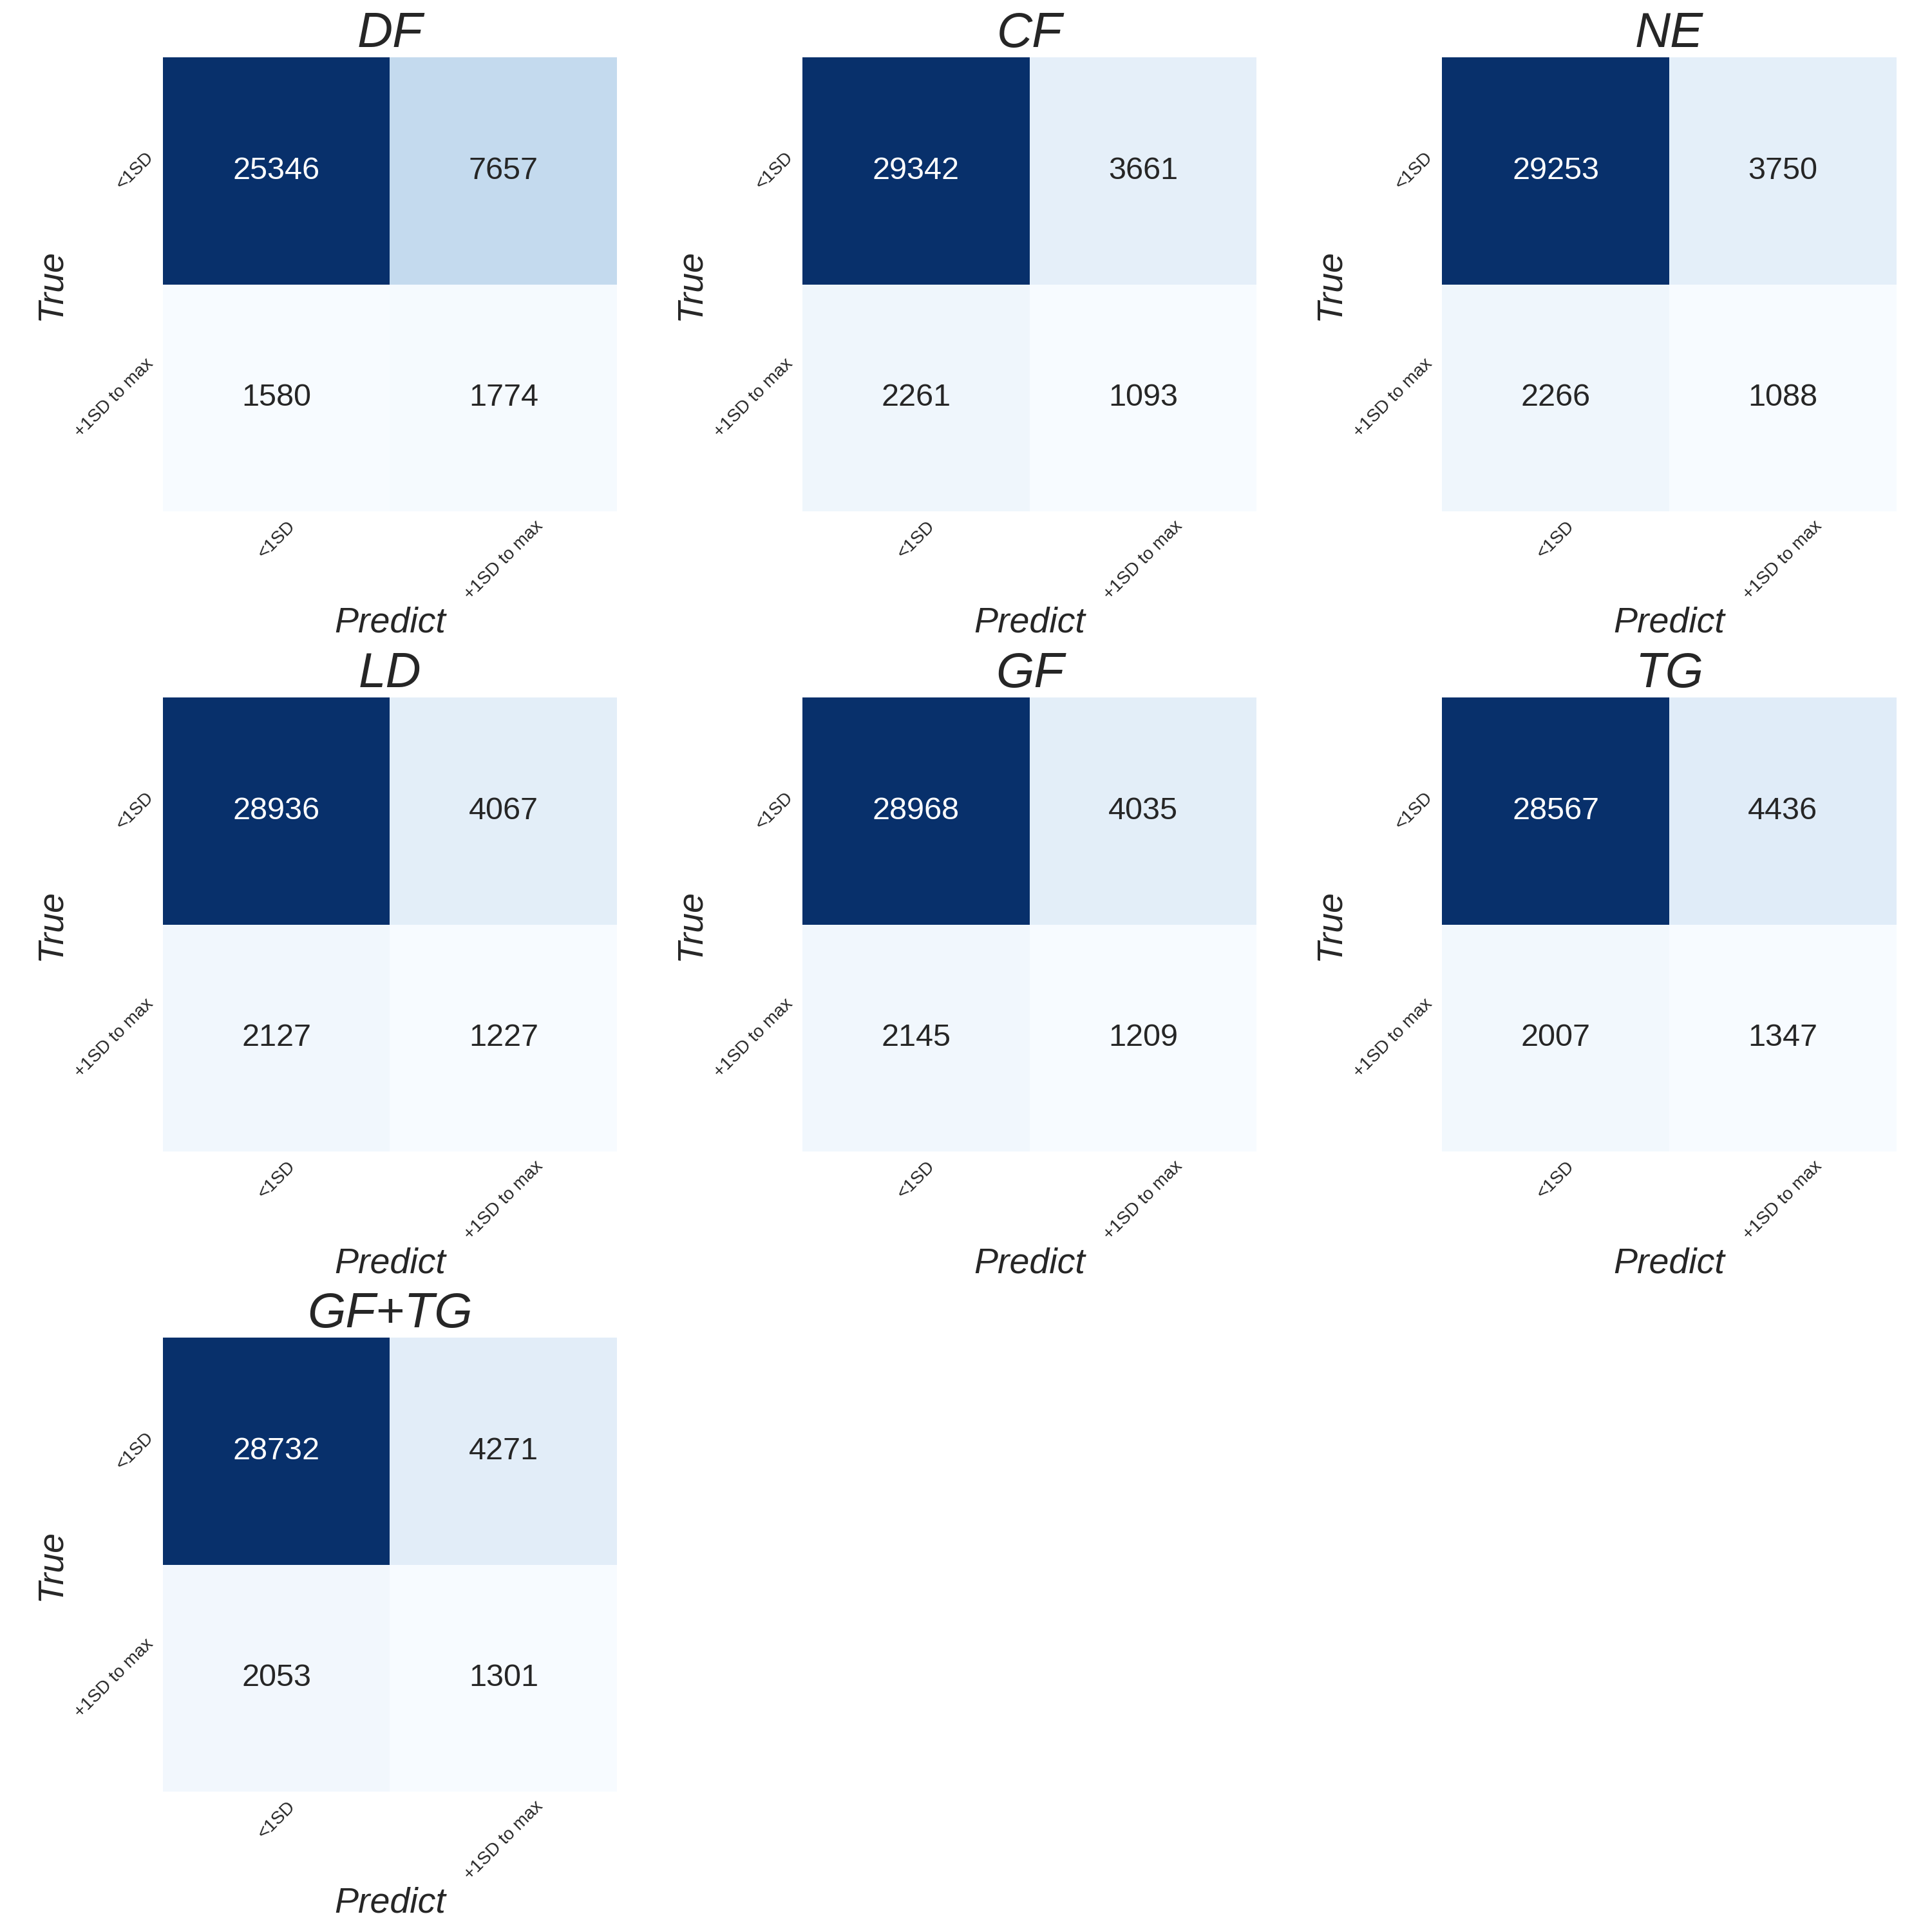
\includegraphics[scale=0.16]{./non-crime-no-timeseries-fig/non_crime_no_timeseries_two_cm.png}
  \caption{2カテゴリーの混同行列}
  \label{fig:non-crime-no-timeseries-2cm}
\end{figure}
% ---------------------------------
% FNFPplot
% ---------------------------------
\begin{figure}
  \centering % 図を中央寄せにする
  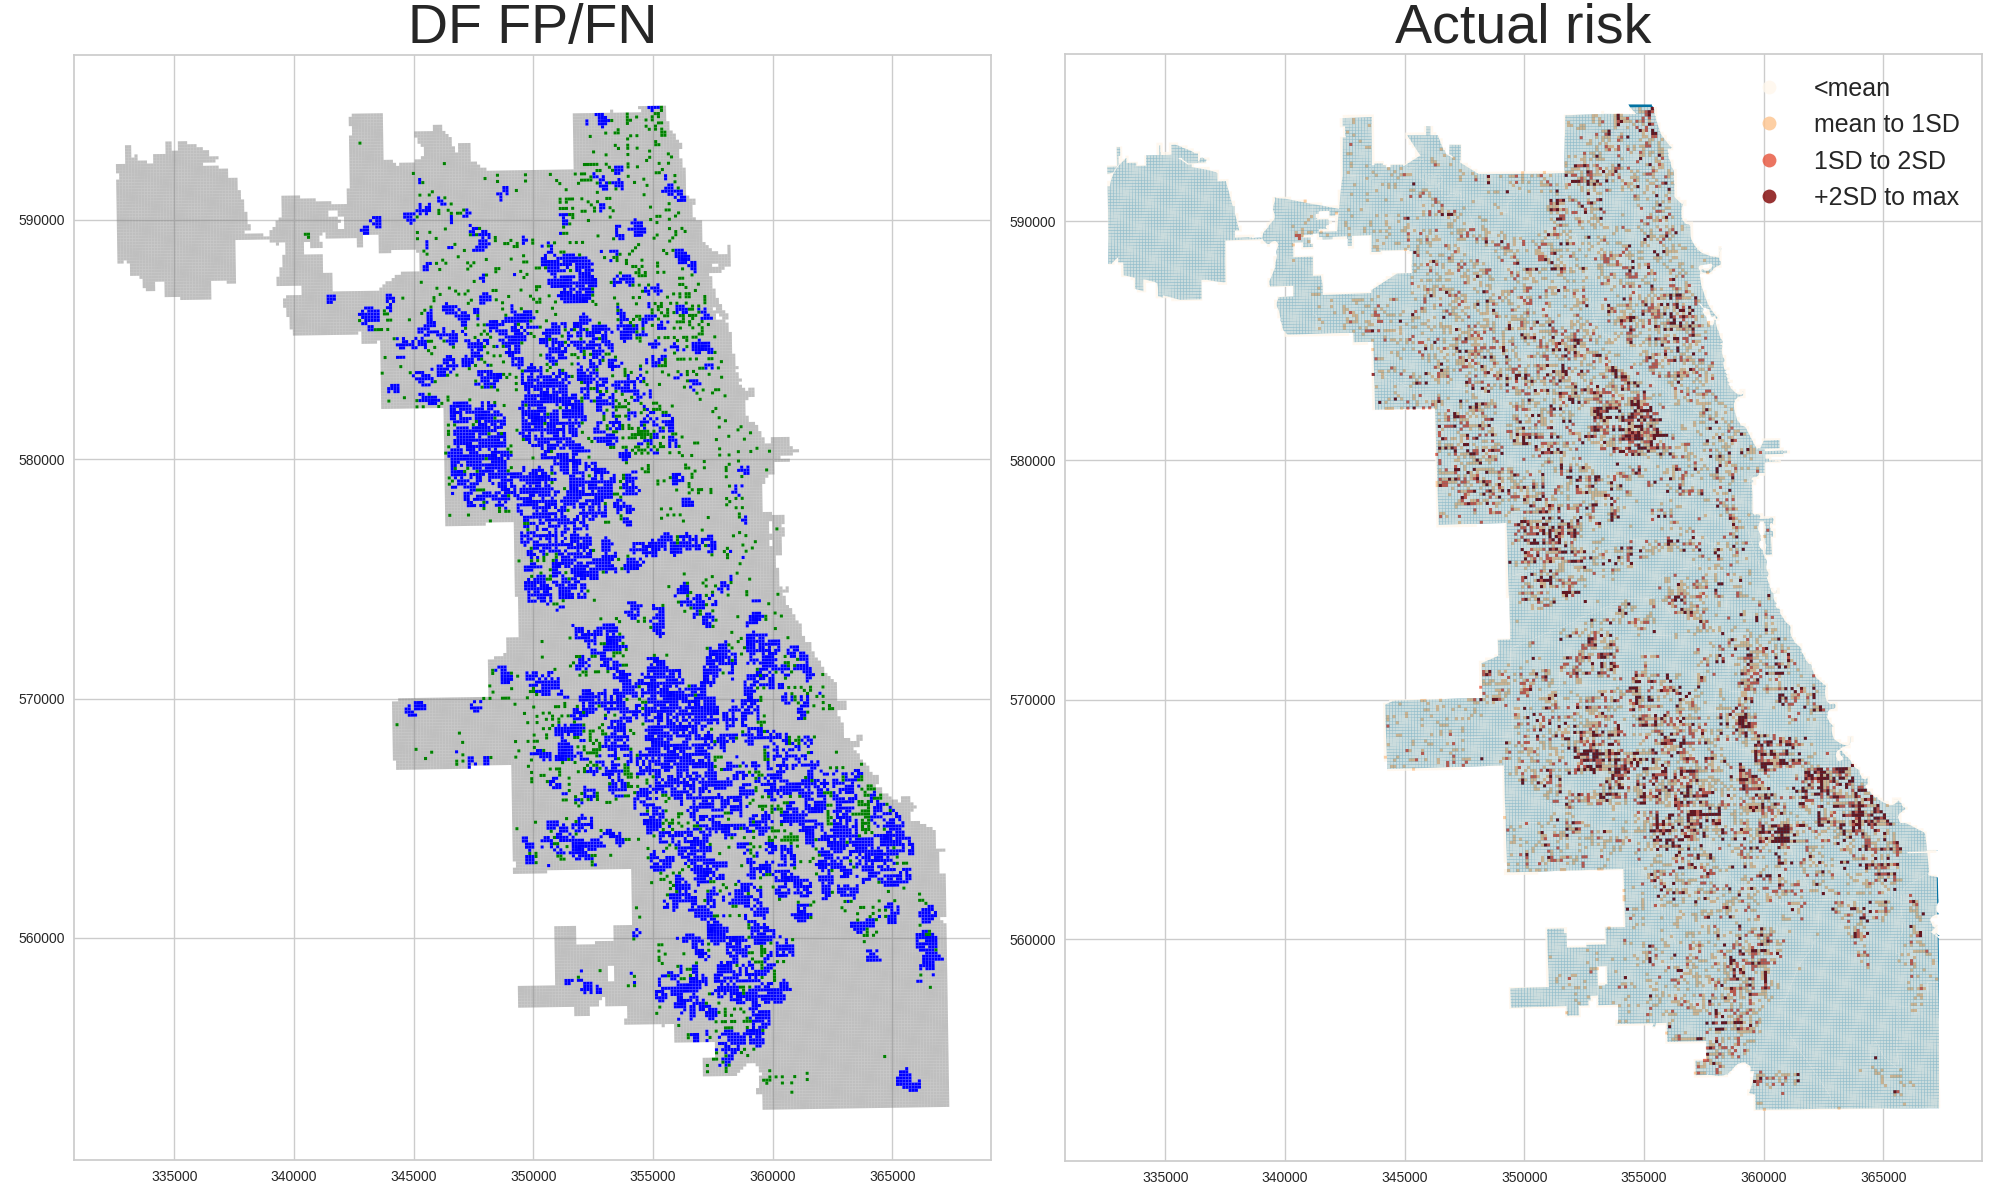
\includegraphics[scale=0.25]{./non-crime-no-timeseries-fig/DF_fnp.png}
  \caption{左:DFのFPFN 右:実際のリスクマップ}
  \label{fig:non-crime-no-timeseries-df-fnp}
\end{figure}

\begin{figure}
  \centering % 図を中央寄せにする
  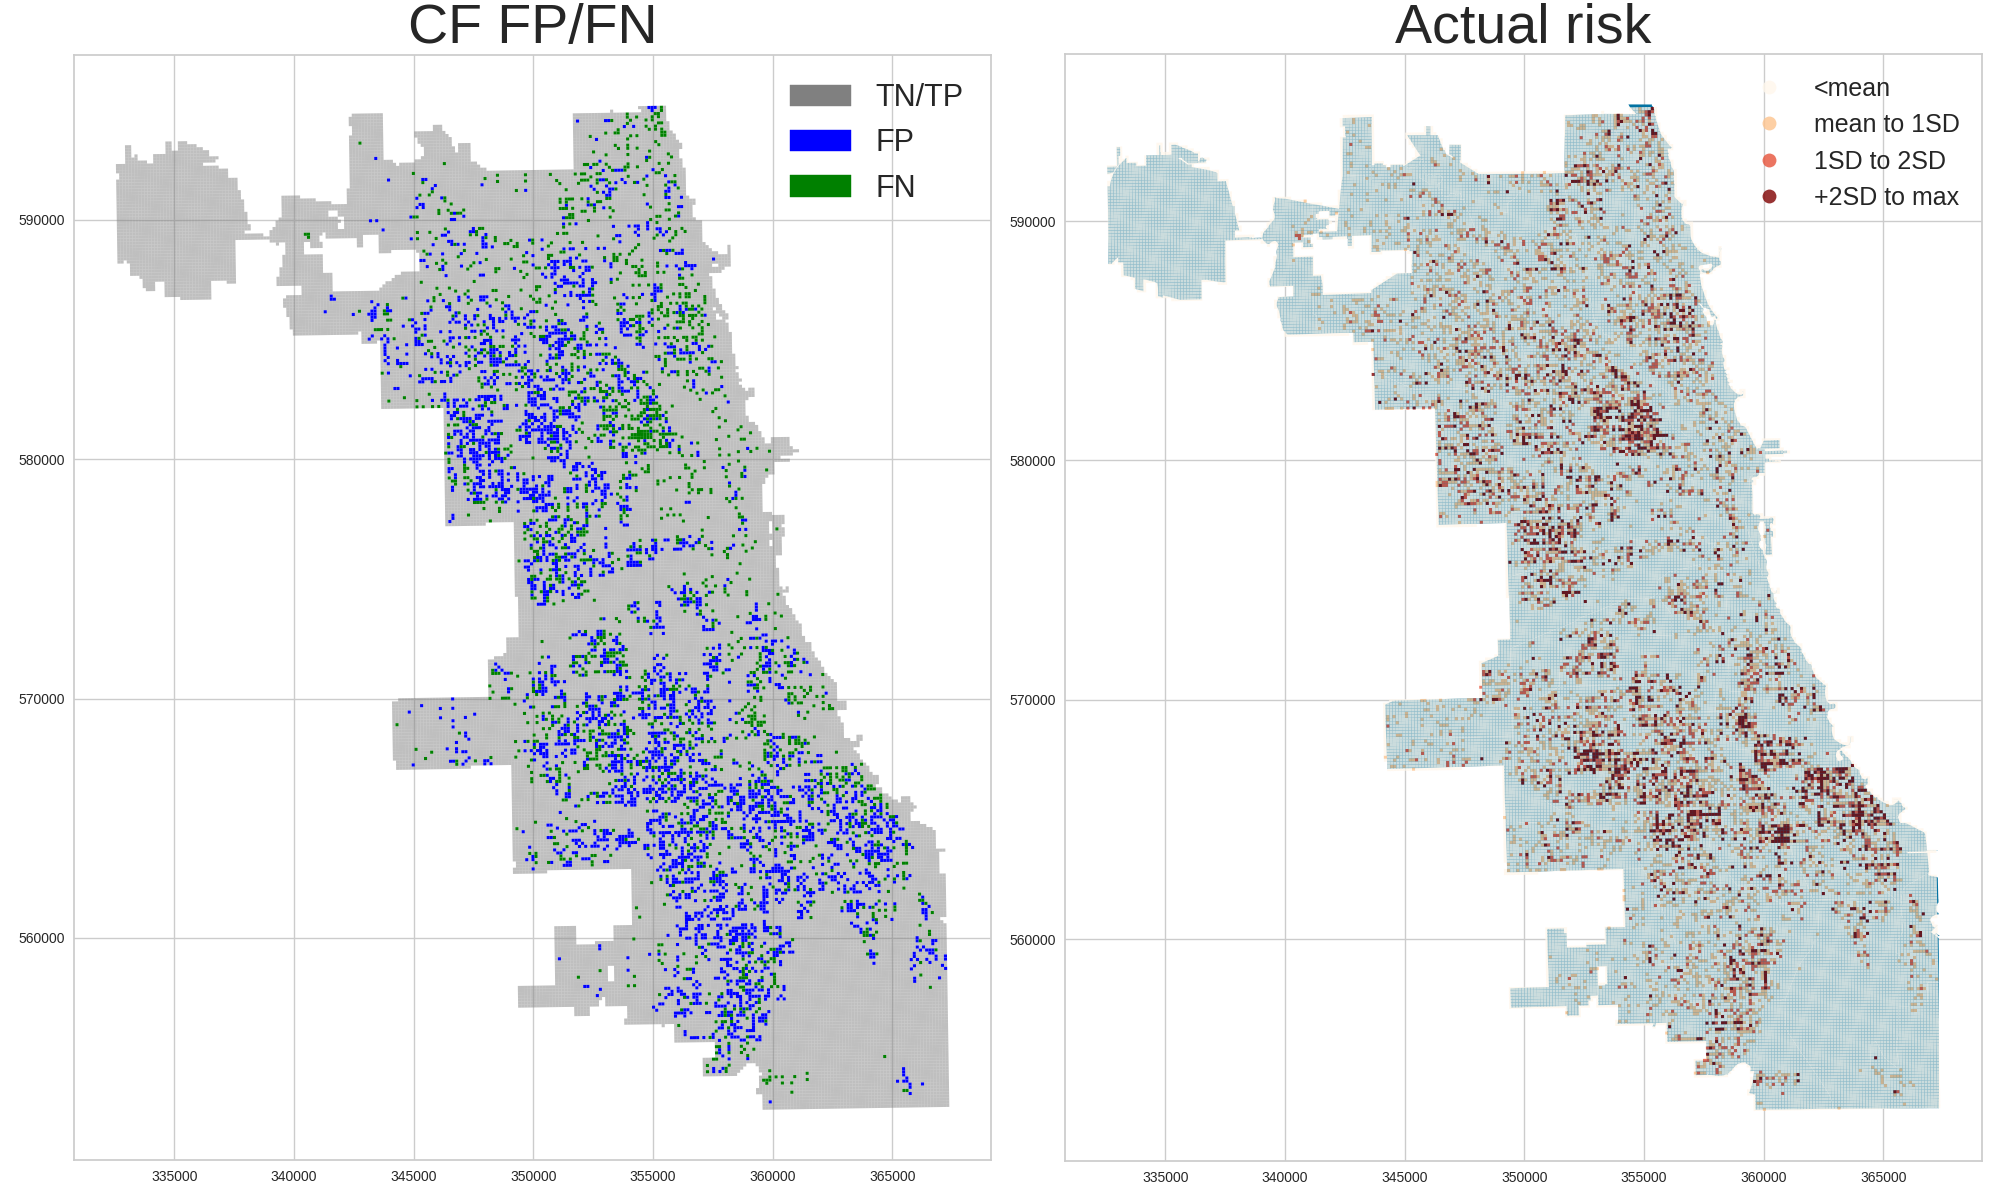
\includegraphics[scale=0.25]{./non-crime-no-timeseries-fig/CF_fnp.png}
  \caption{左:CFのFPFN 右:実際のリスクマップ}
  \label{fig:non-crime-no-timeseries-cf-fnp}
\end{figure}

\begin{figure}
  \centering % 図を中央寄せにする
  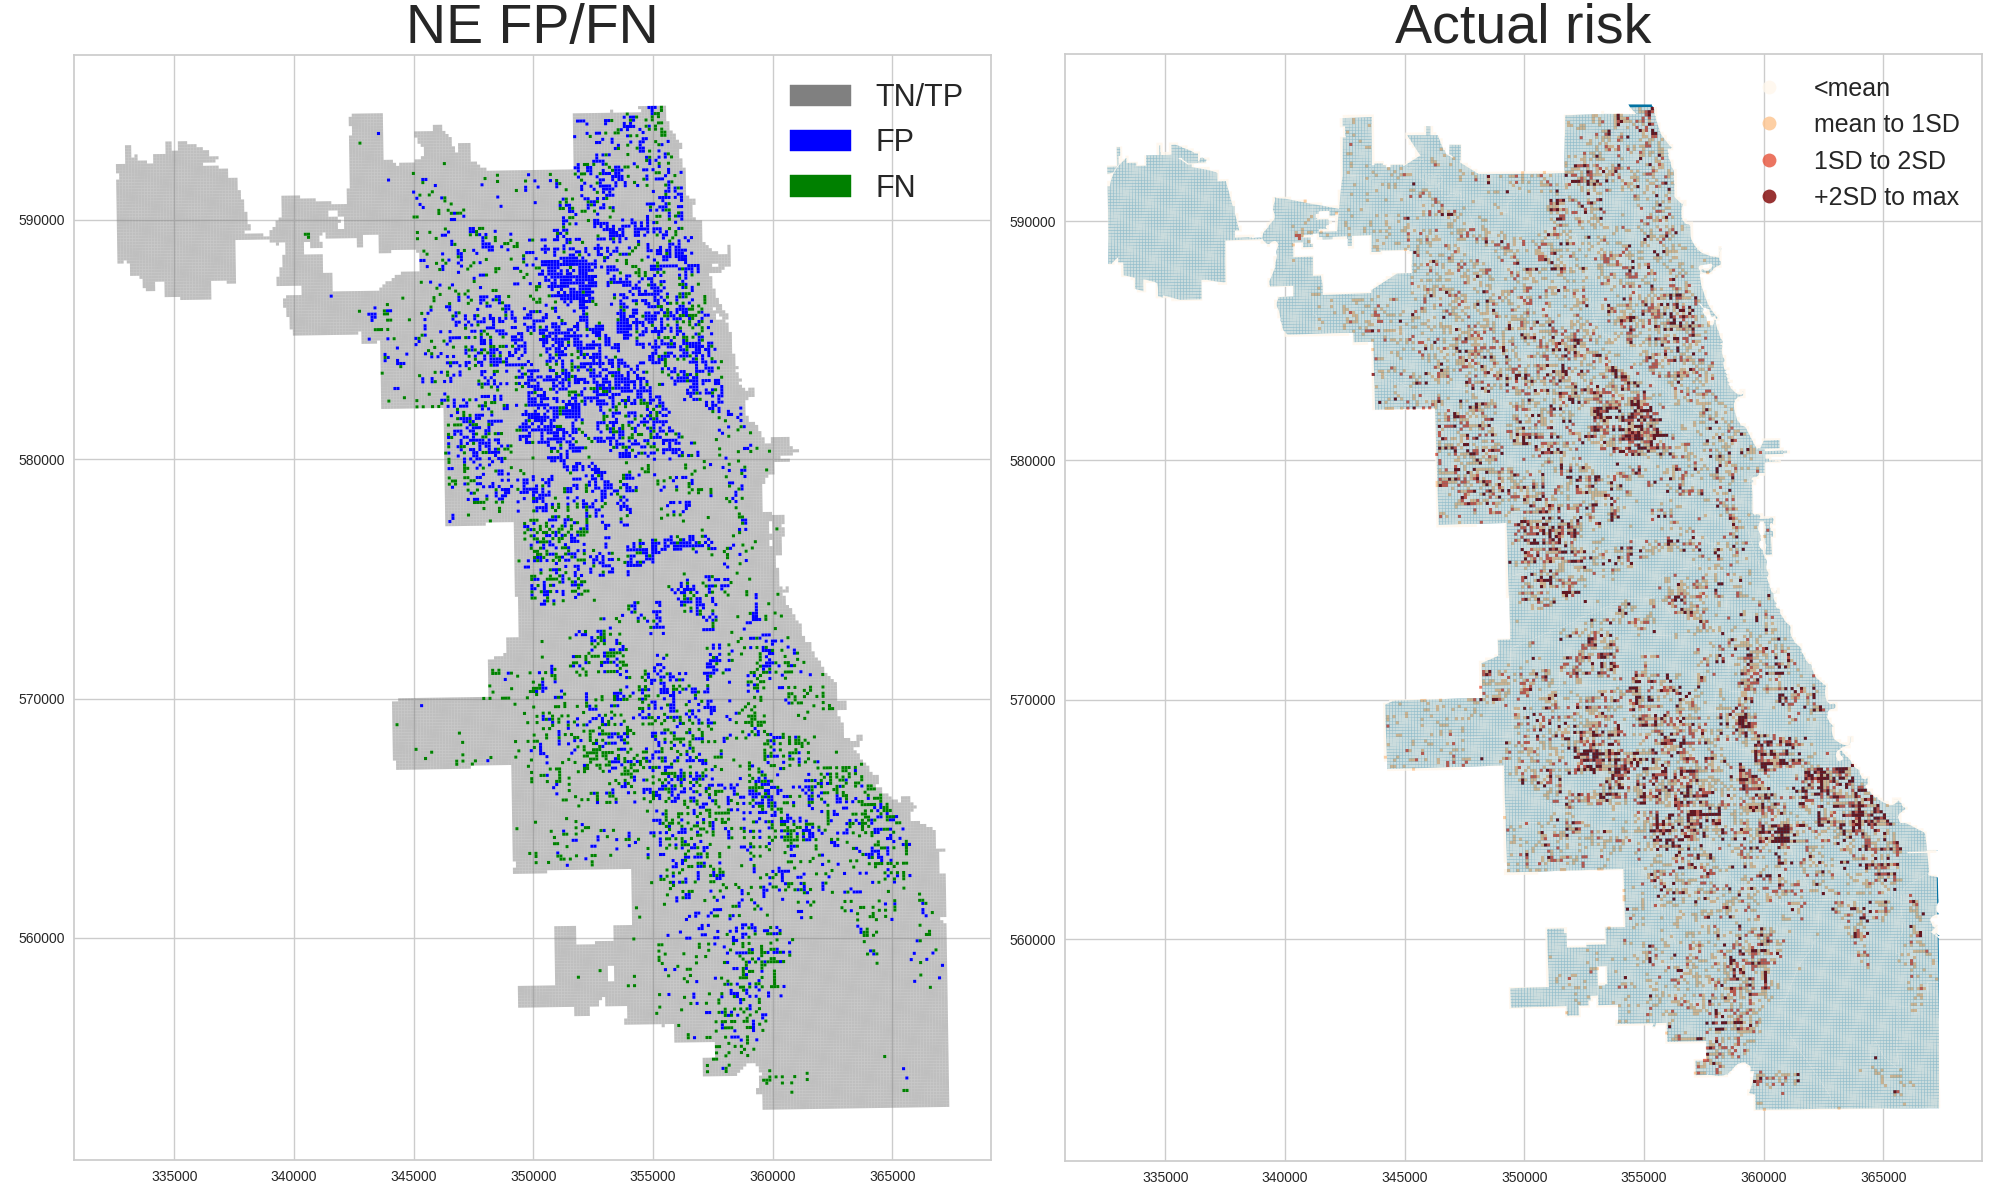
\includegraphics[scale=0.25]{./non-crime-no-timeseries-fig/NE_fnp.png}
  \caption{左:NEのFPFN 右:実際のリスクマップ}
  \label{fig:non-crime-no-timeseries-ne-fnp}
\end{figure}

\begin{figure}
  \centering % 図を中央寄せにする
  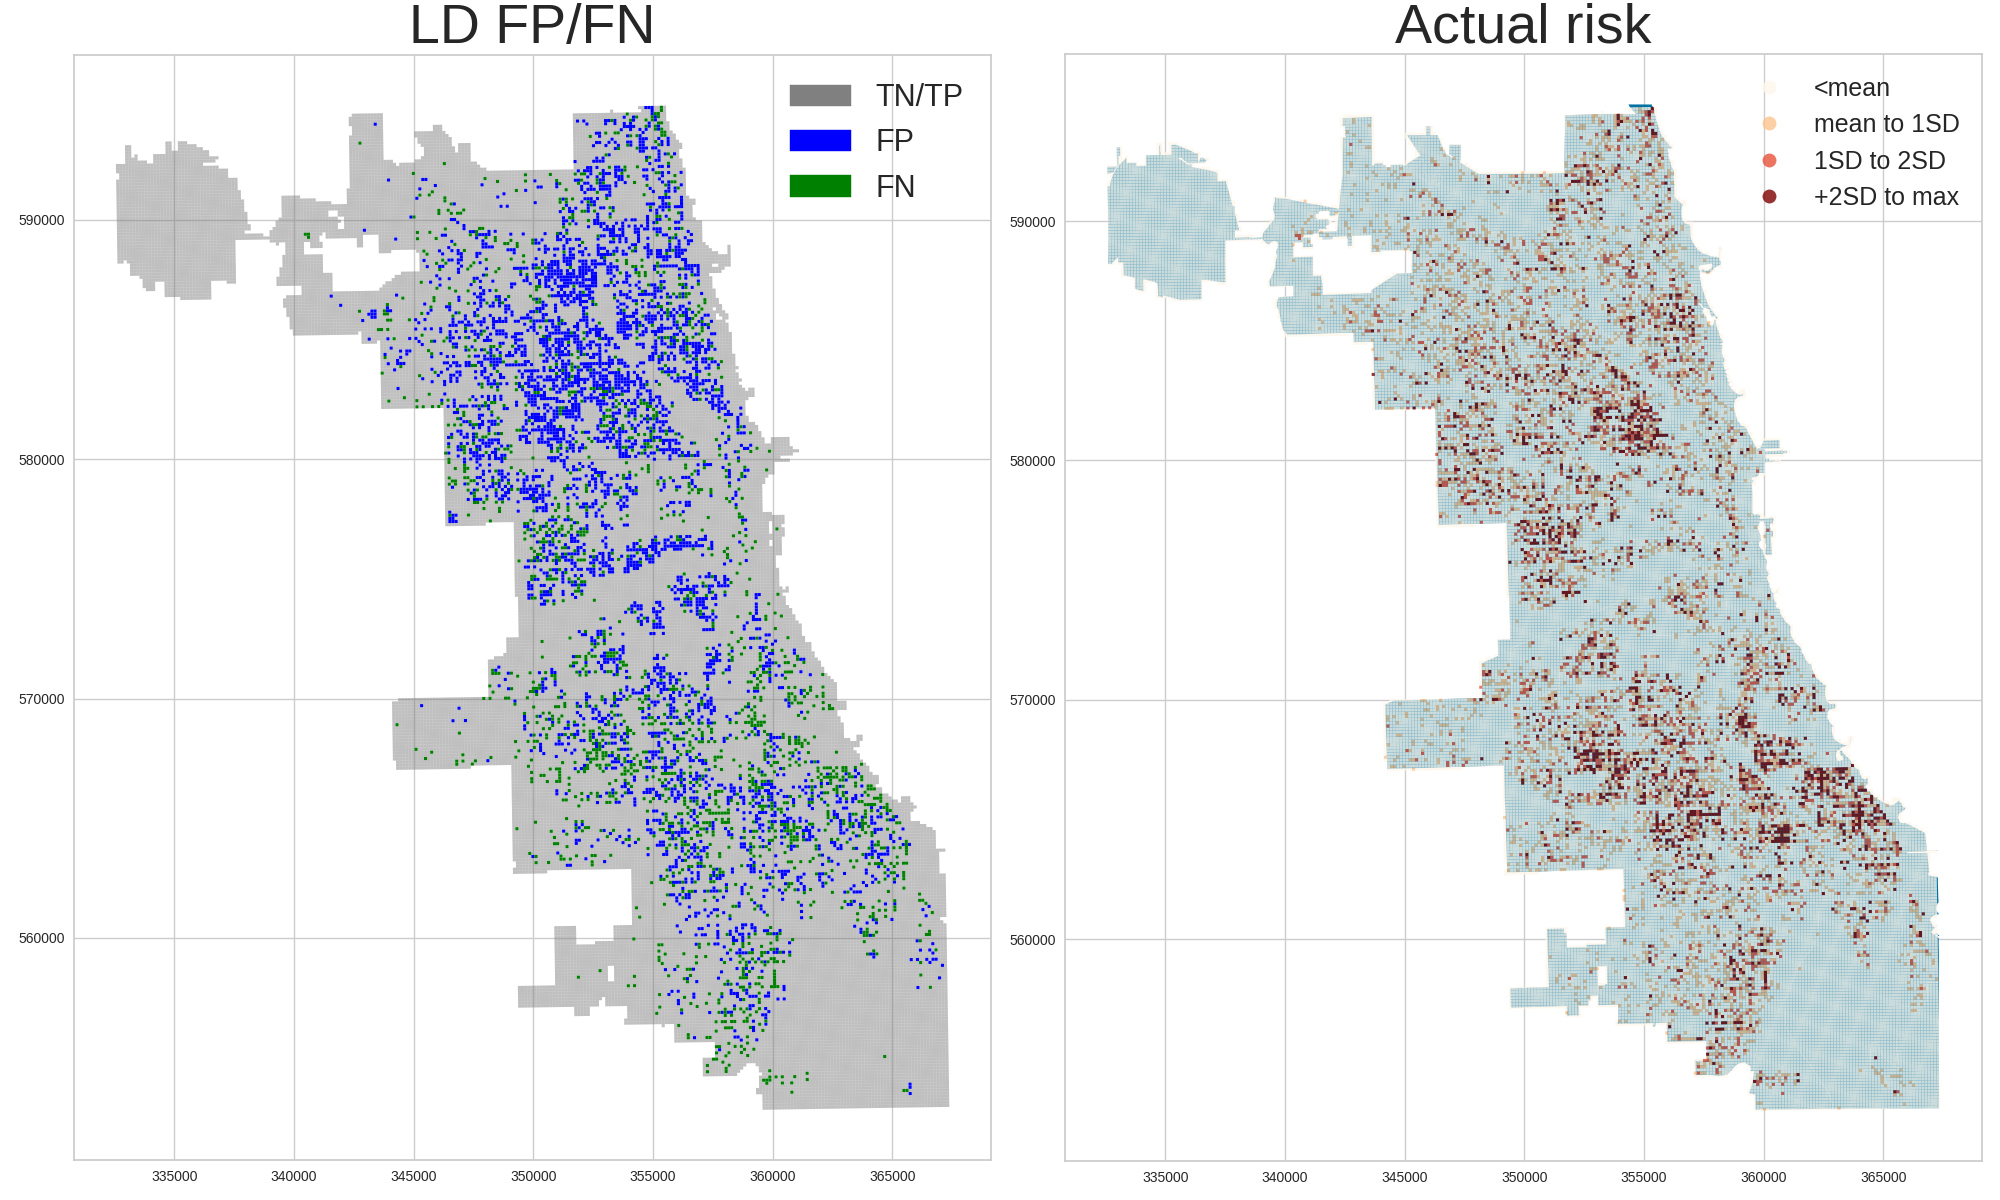
\includegraphics[scale=0.25]{./non-crime-no-timeseries-fig/LD_fnp.png}
  \caption{左:LDのFPFN 右:実際のリスクマップ}
  \label{fig:non-crime-no-timeseries-ld-fnp}
\end{figure}

\begin{figure}
  \centering % 図を中央寄せにする
  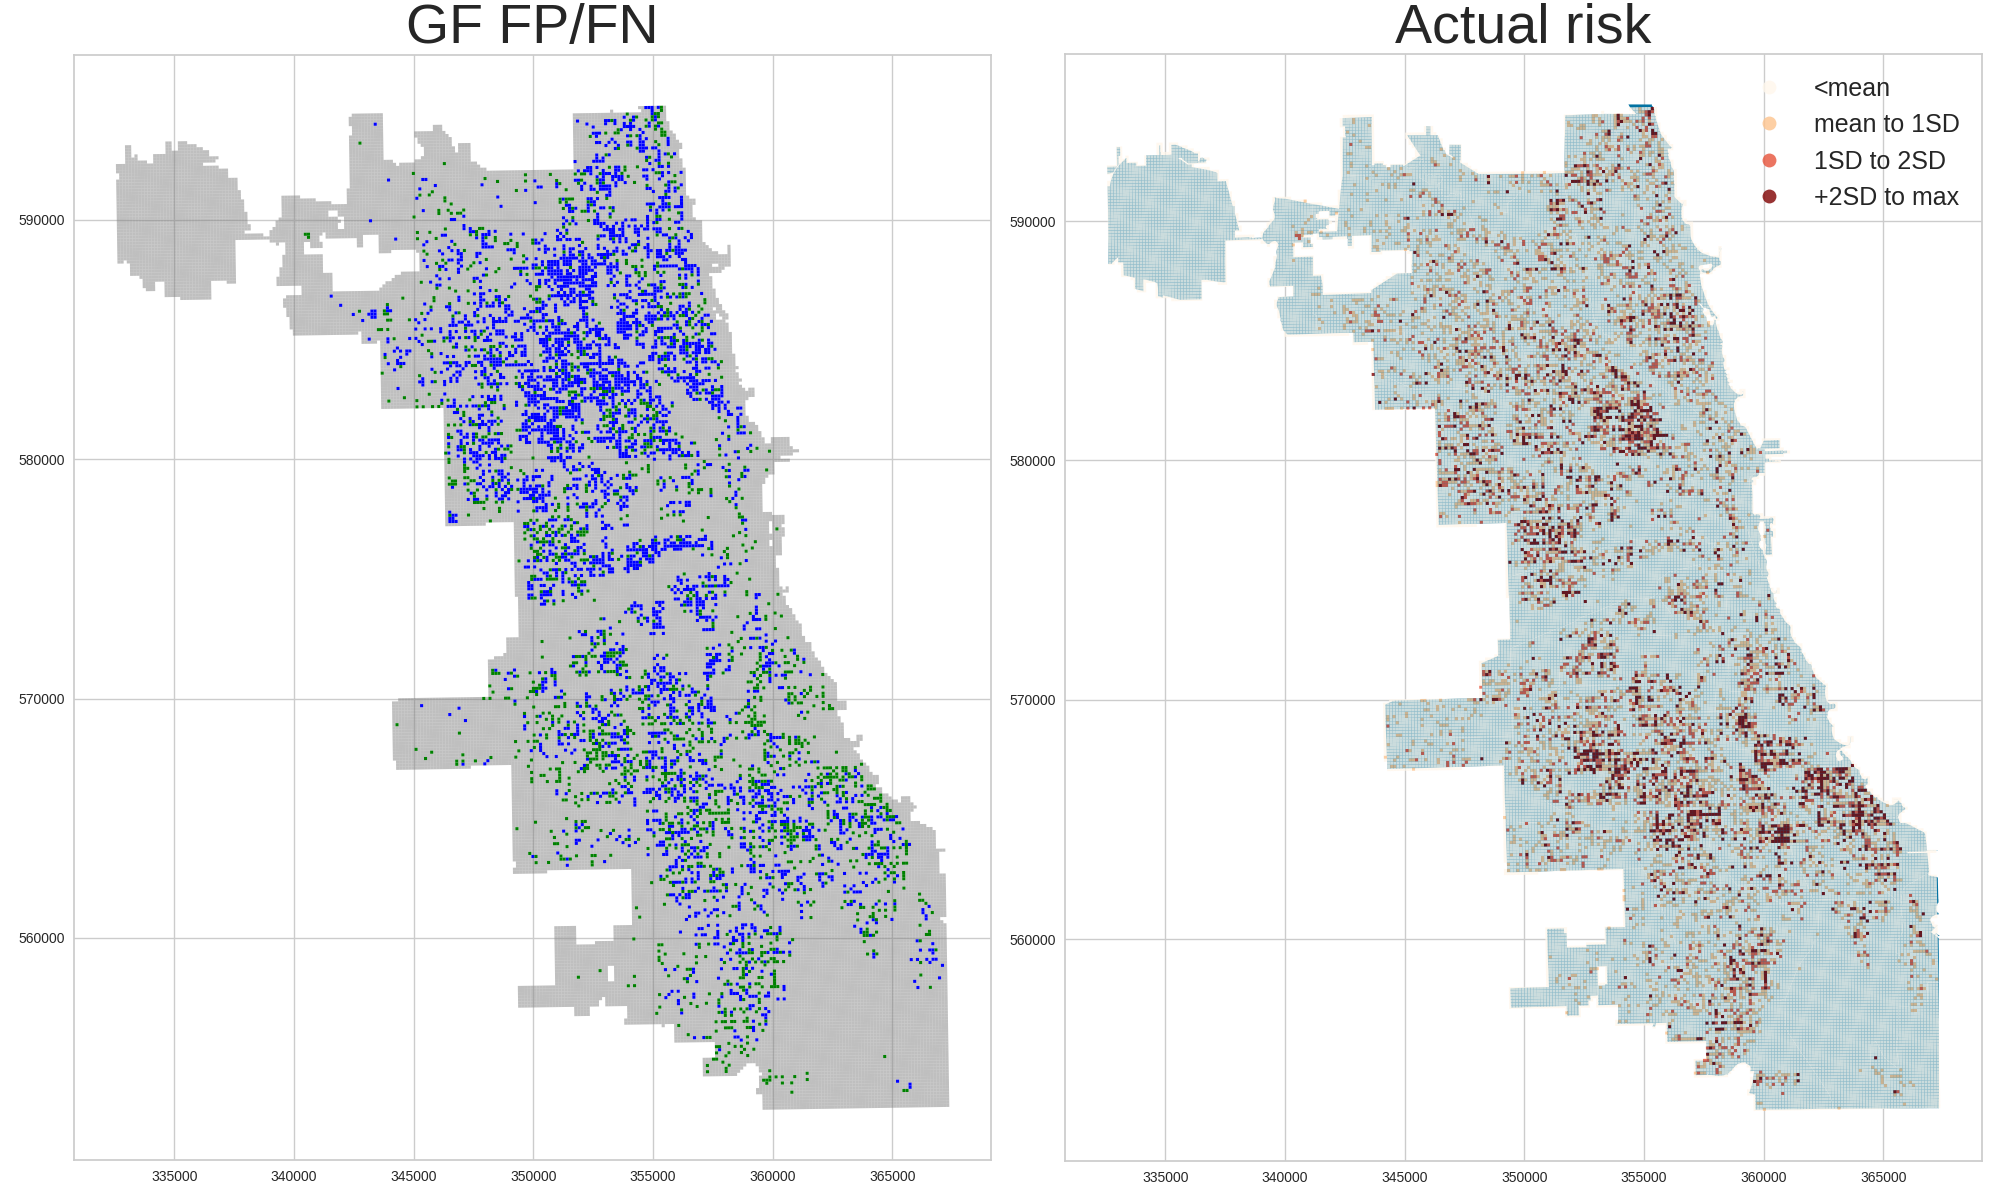
\includegraphics[scale=0.25]{./non-crime-no-timeseries-fig/GF_fnp.png}
  \caption{左:GFのFPFN 右:実際のリスクマップ}
  \label{fig:non-crime-no-timeseries-gf-fnp}
\end{figure}

\begin{figure}
  \centering % 図を中央寄せにする
  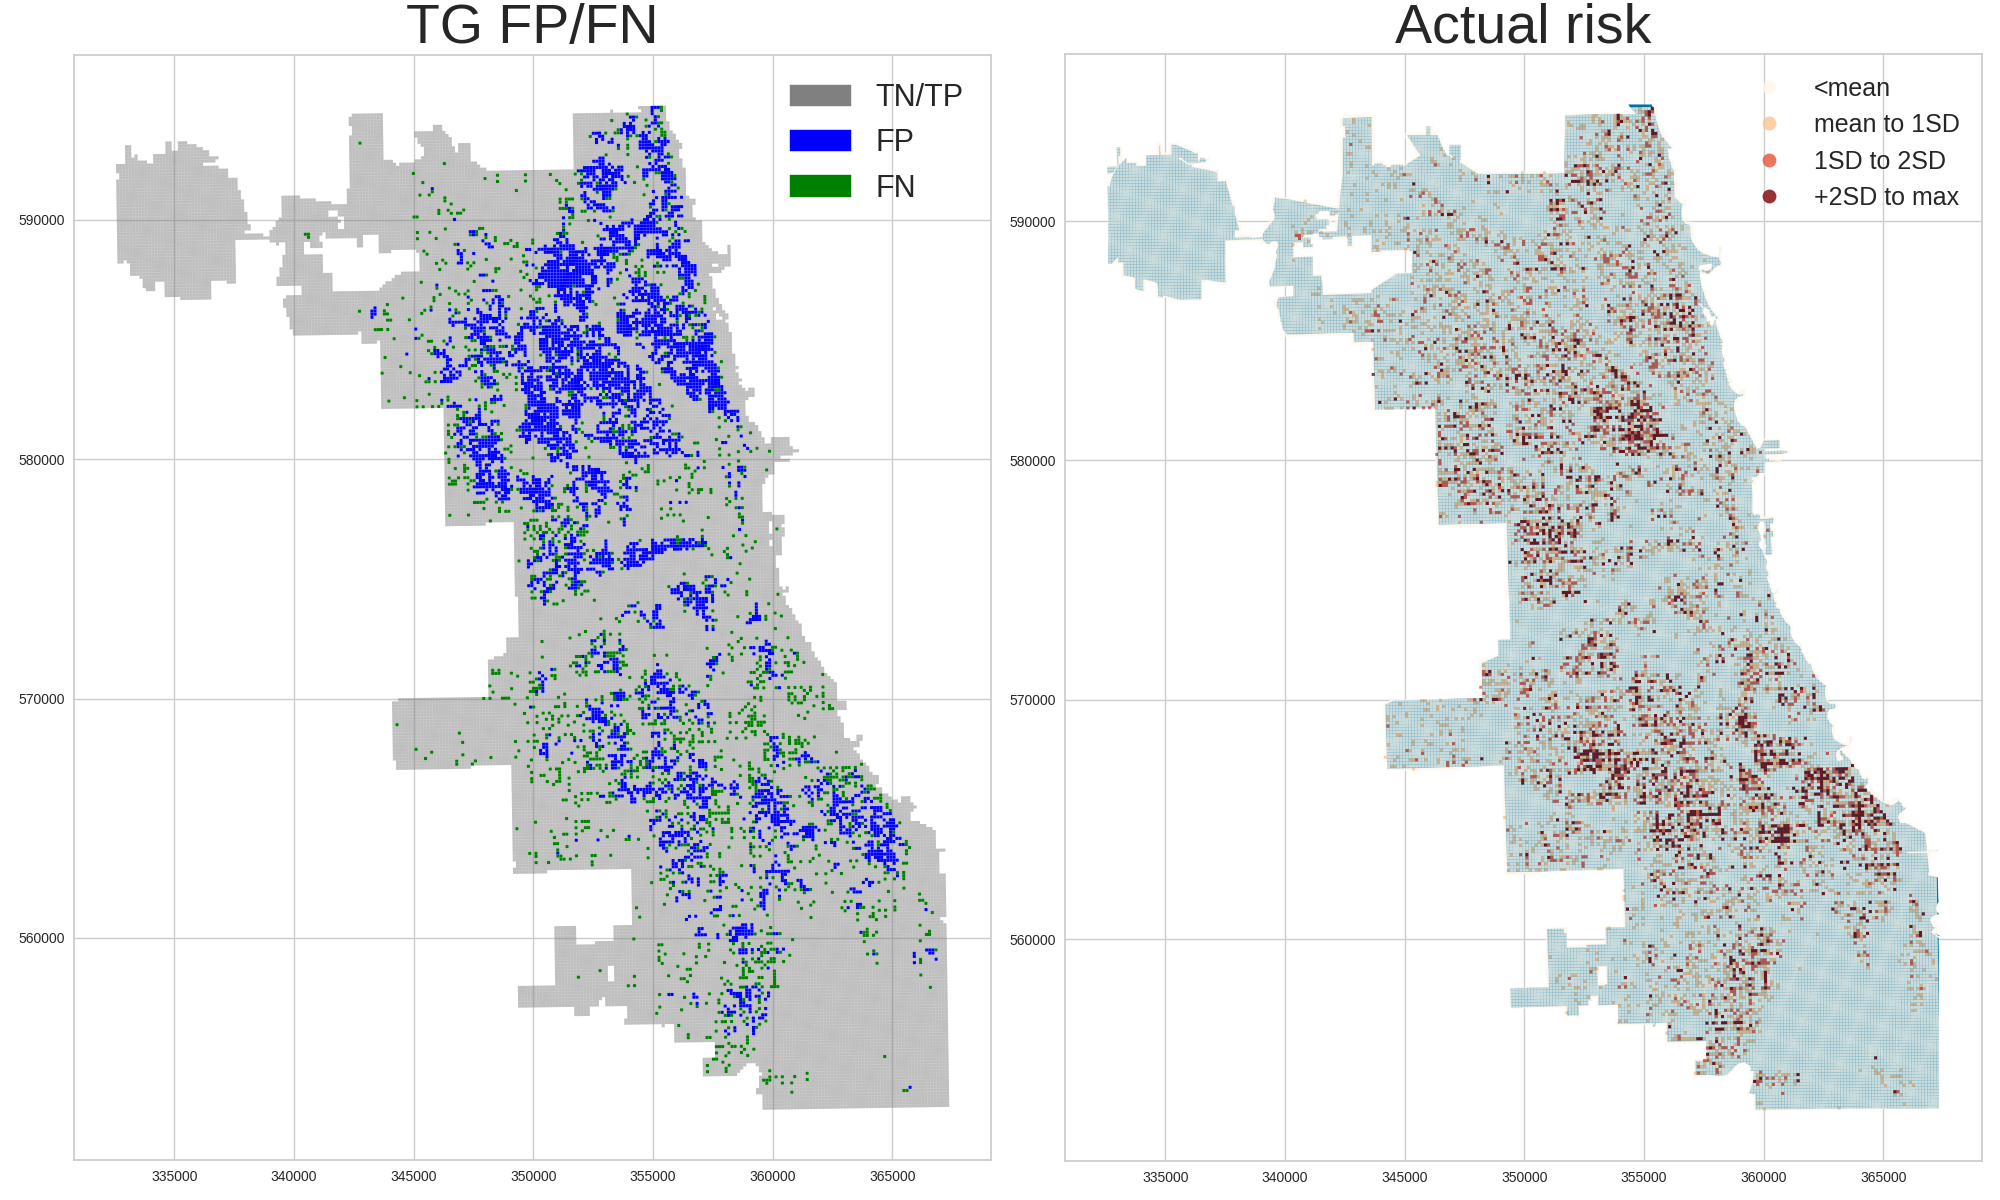
\includegraphics[scale=0.25]{./non-crime-no-timeseries-fig/TG_fnp.png}
  \caption{左:TGのFPFN 右:実際のリスクマップ}
  \label{fig:non-crime-no-timeseries-tg-fnp}
\end{figure}

\begin{figure}
  \centering % 図を中央寄せにする
  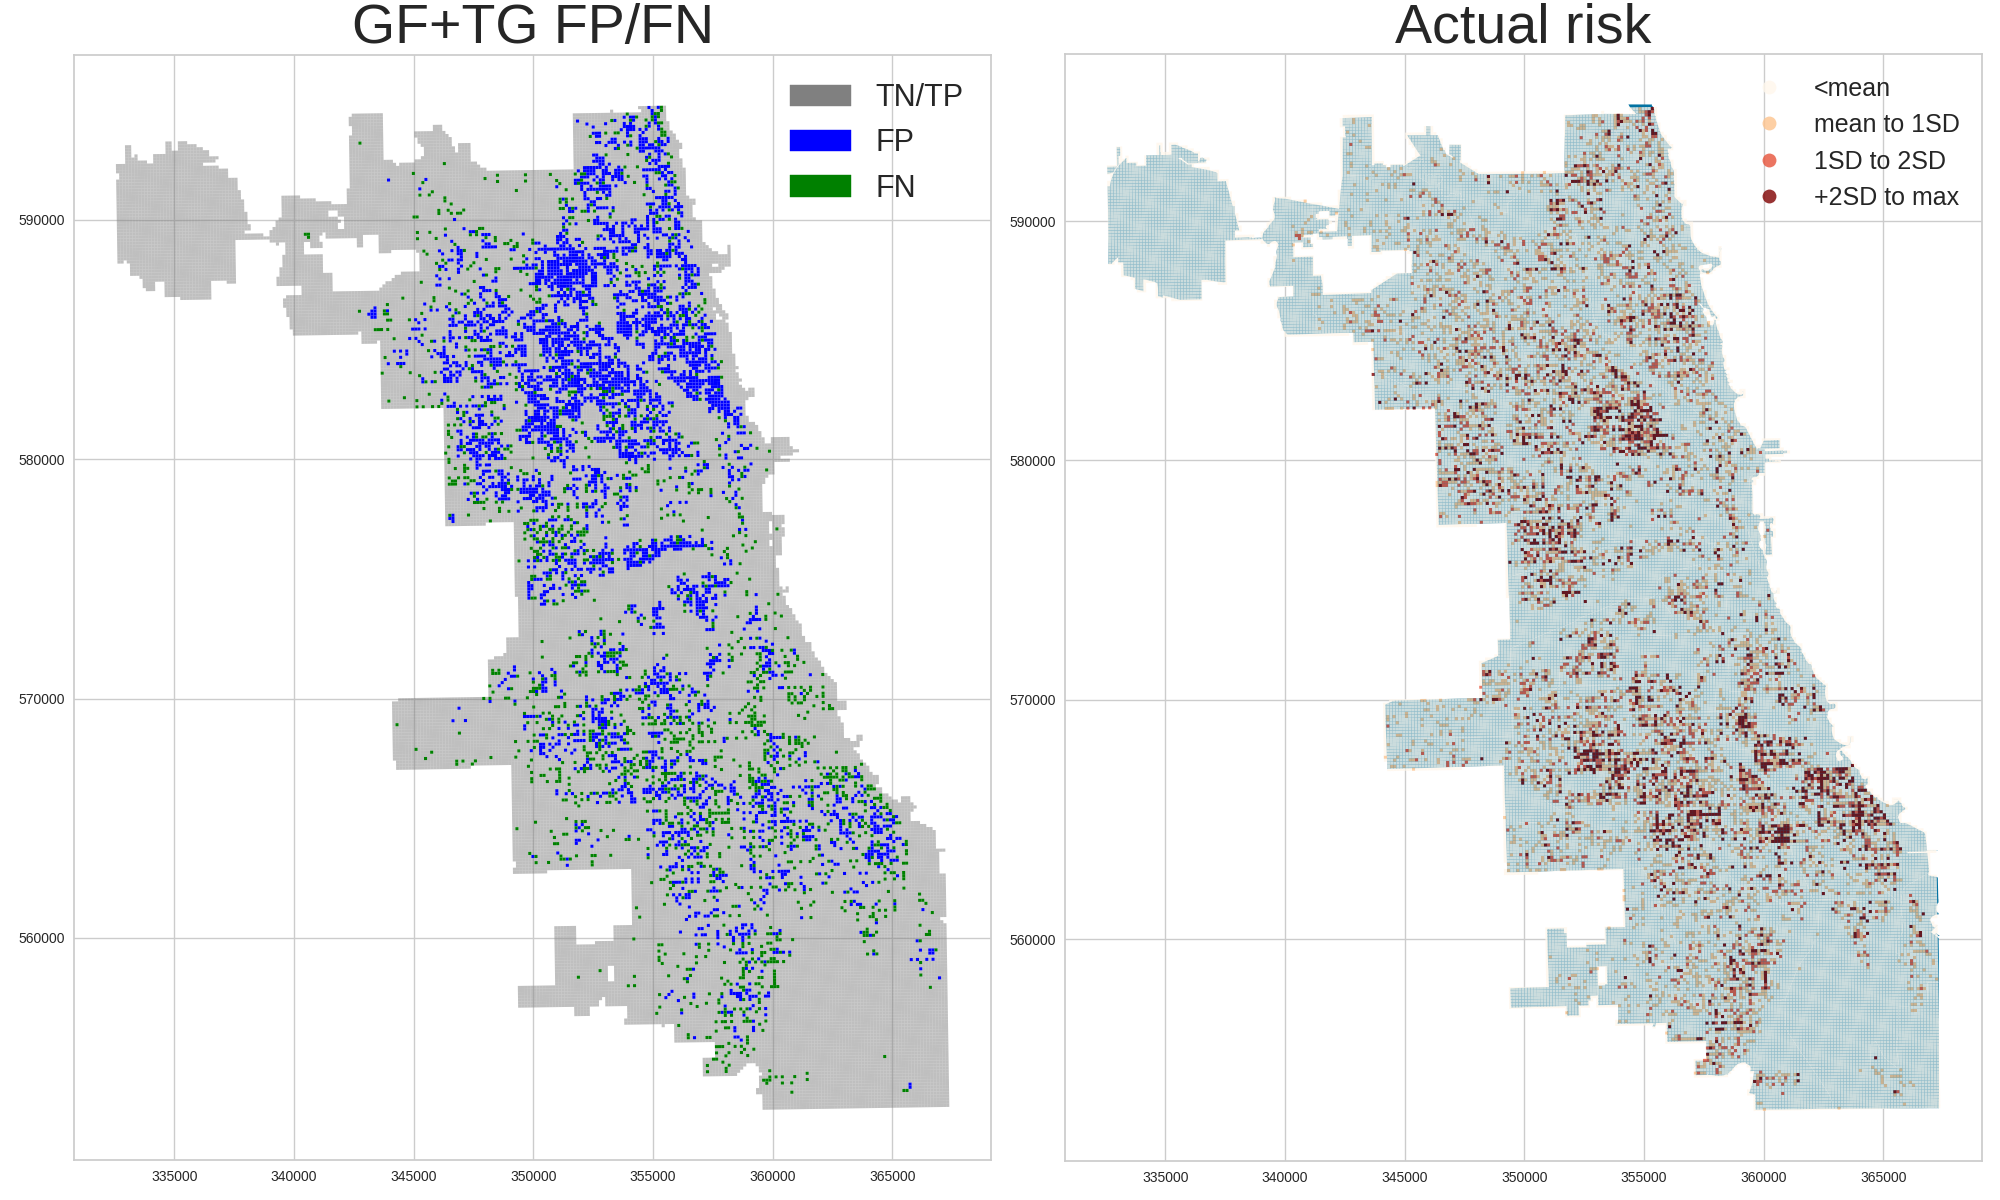
\includegraphics[scale=0.25]{./non-crime-no-timeseries-fig/GF+TG_fnp.png}
  \caption{左:GF+TGのFPFN 右:実際のリスクマップ}
  \label{fig:non-crime-no-timeseries-gf-tg-fnp}
\end{figure}
%------------------------------------------
% ROC curve
%------------------------------------------
また,各モデルのROC曲線を図\ref{fig:non-crime-no-timeseries-roc}に示した.

\begin{figure}
  \centering % 図を中央寄せにする
  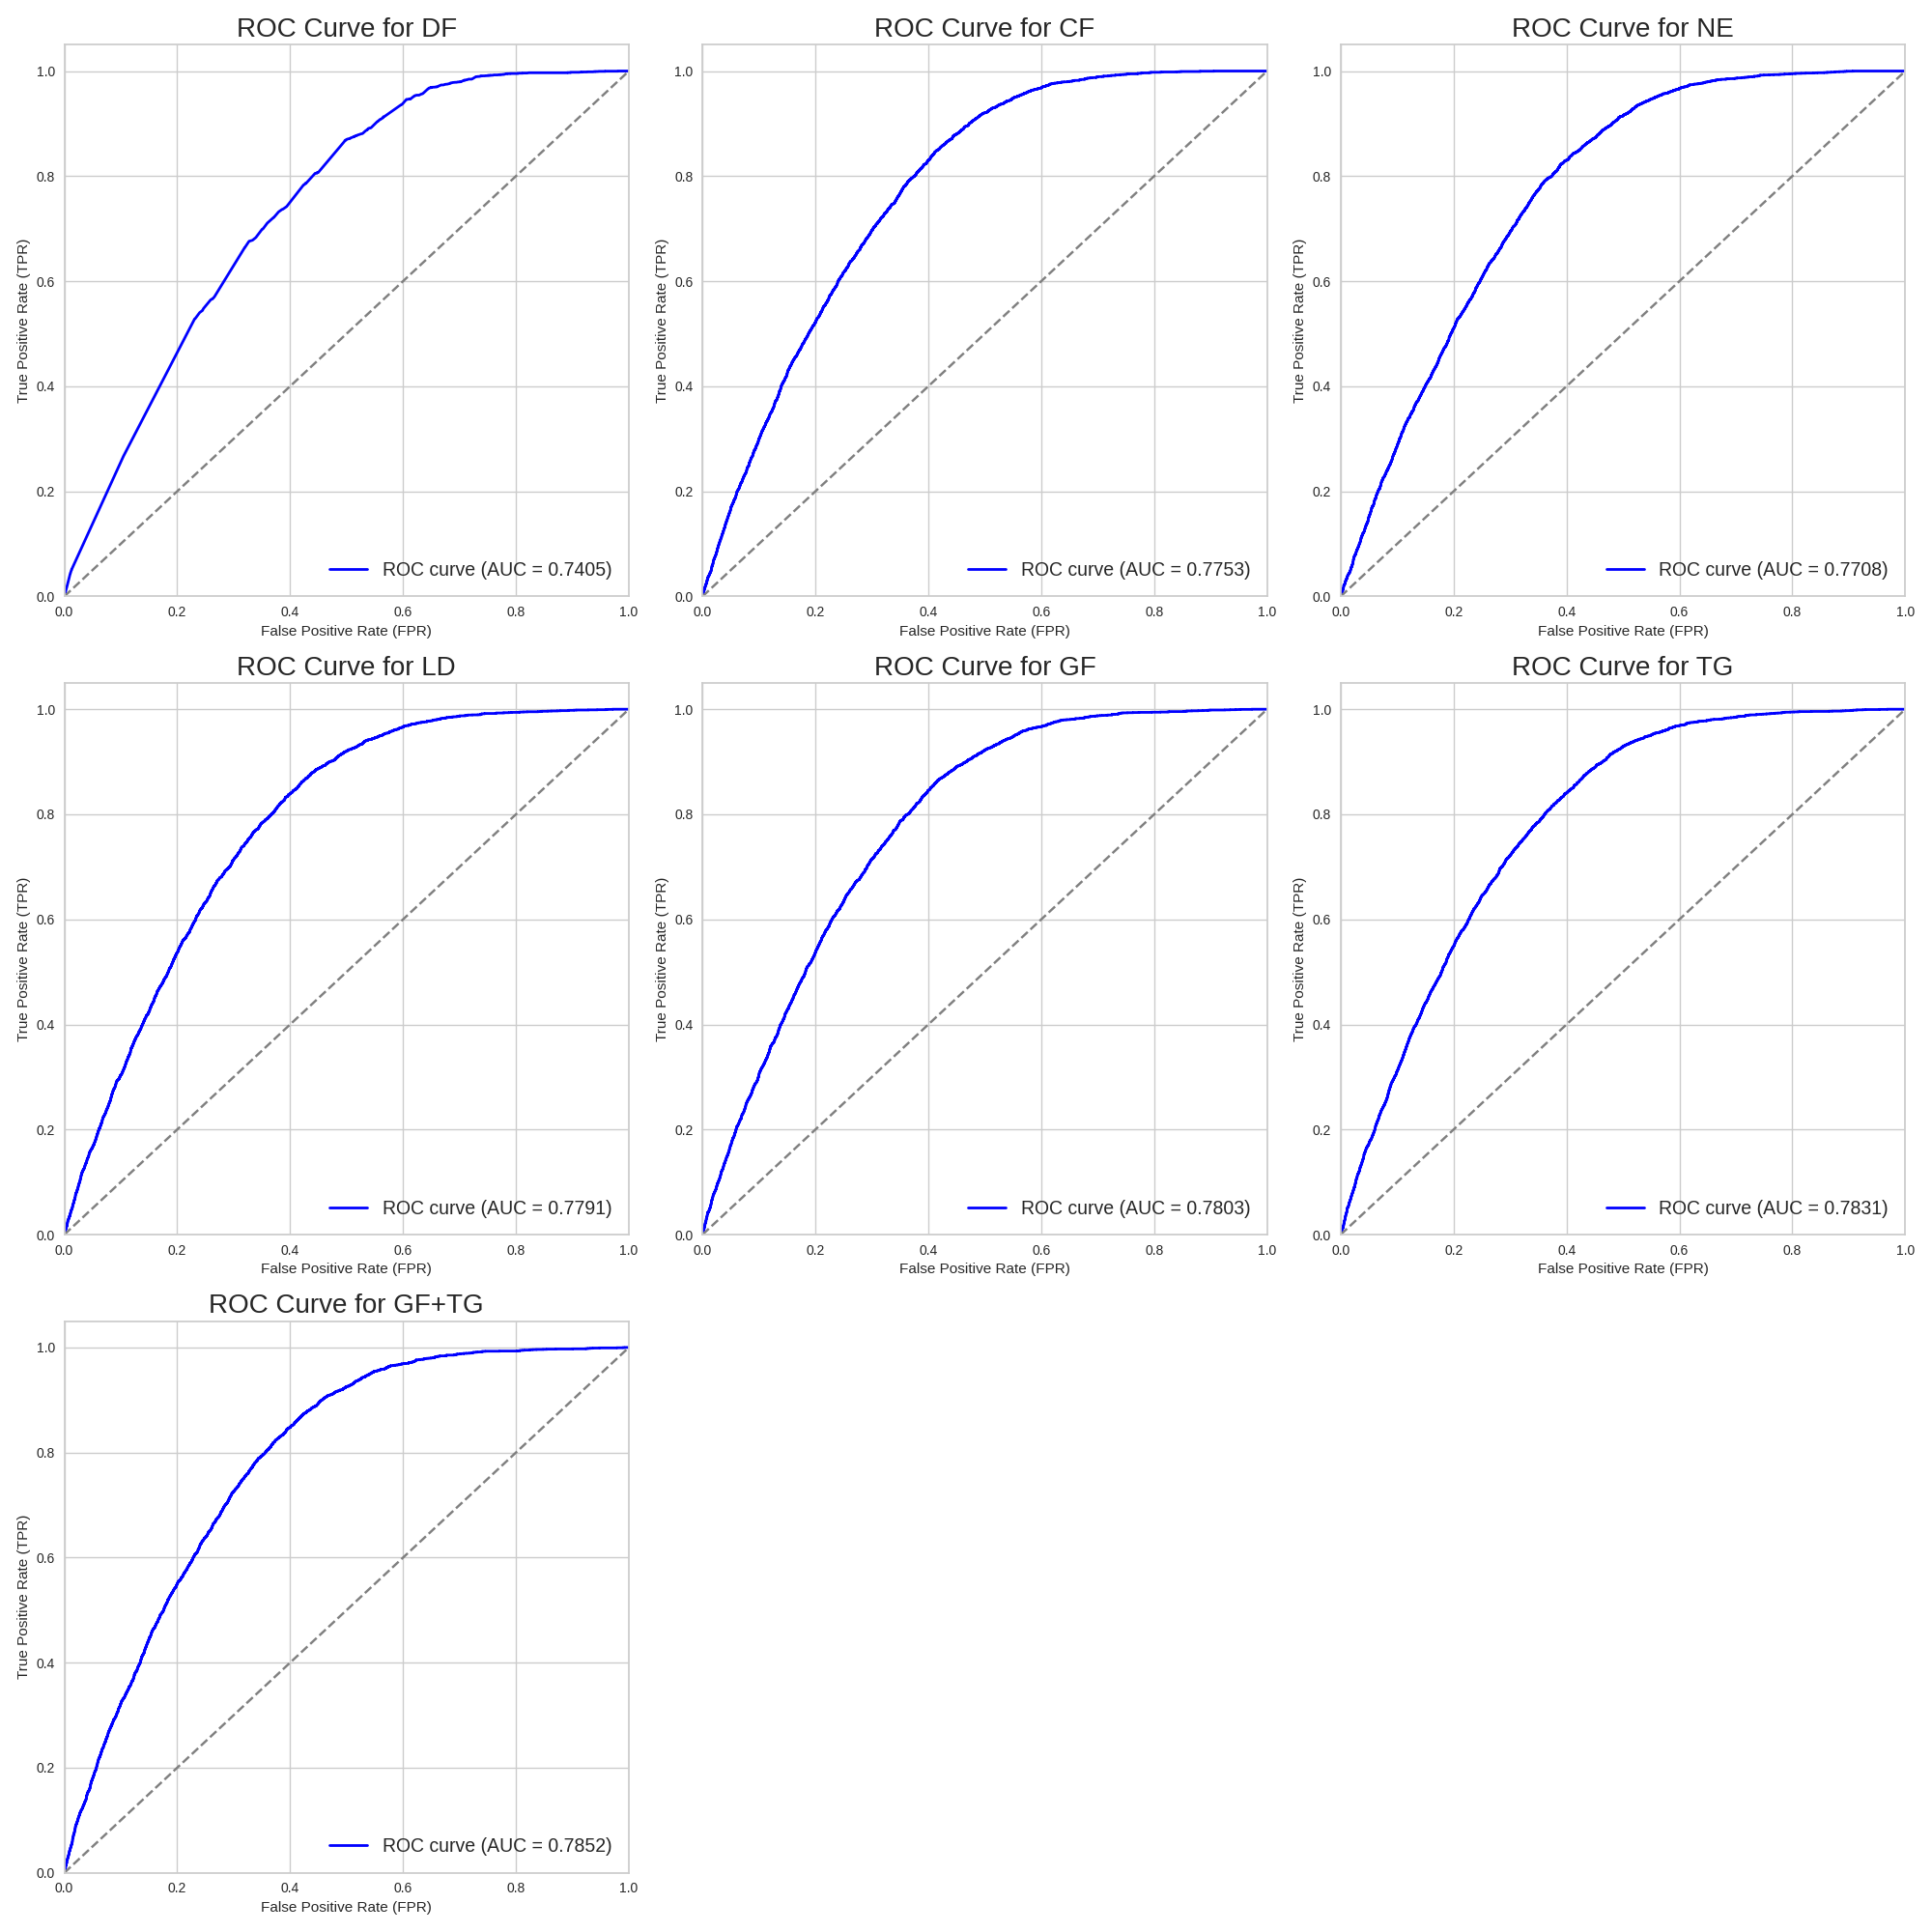
\includegraphics[scale=0.25]{./non-crime-no-timeseries-fig/roc_auc.png}
  \caption{ROC曲線}
  \label{fig:non-crime-no-timeseries-roc}
\end{figure}
%------------------------------------------
% table
%------------------------------------------
各モデルの予測精度を精度指標を基に比較した結果を表\ref{tb:non-crime-no-timeseries-index}にまとめる.

\begin{table}[htbp]
  \centering
  \caption{各モデル間の精度比較}
  \begin{tabular}{l|r|r|r|r|r|r|r}
  \hline

  モデル & DF & CF & NE & LD & GF & TG & GF+TG \\  \hline\hline
的中率 & 50.2 & 30.7 & 30.3 & 34.4 & 34.1 & 38.1 & 36.9 \\ 
PAI & 1.93 & 2.35 & 2.28 & 2.36 & 2.36 & 2.40 & 2.41 \\ 
AUC & 0.74 & 0.78 & 0.77 & 0.78 & 0.78 & 0.78 & 0.79 \\ \hline


  \end{tabular}
  \label{tb:non-crime-no-timeseries-index}
\end{table}

\FloatBarrier
%------------------------------------
\section{時系列に配慮した方法}
%------------------------------------
時系列に配慮しない方法では,未来の地理的リスク要因の情報を犯罪発生リスクの予測に用いていた.
そこで時系列に配慮した方法を提案し,この方法についても同様に各モデルに対して予測精度を比較する.
%------------------------------------
\subsection{実験条件}
%------------------------------------
学習データとテストデータの構成を,1年ずつ予測変数と応答変数の対をずらすことで,予測に未来の情報を用いないようにする.
学習データの構成は,2011年の地理的リスク要因を予測変数としてそれに対する応答変数を2012年に発生した強盗犯罪とする.
これに加えて,2012年の地理的リスク要因を予測変数として,それに対する応答変数を2012年に発生した強盗犯罪とする.
この計2年分の予測変数と応答変数の対を学習データとする.
またテストデータは,2013年の地理的リスク要因を予測変数としてそれに対する応答変数を2014年に発生した強盗犯罪とする.
%------------------------------------
\subsection{結果}
%------------------------------------

\ref{non-crime-no-timeseries-result}同様に予測結果を示す.

2014年に実際に起った強盗犯罪の発生地点とそれに基づいた実際のリスクマップを
図\ref{fig:non-crime-timeseries-actual-risk}に示す.
DFによる予測結果を図\ref{fig:non-crime-timeseries-df-risk}に,
CFによる予測結果を図\ref{fig:non-crime-timeseries-cf-risk}に示す.
実際のリスクマップと比べて,離散型特徴量によるリスクマップでは高い空間相関を持つが,
連続型特徴量によるリスクマップは空間相関が削減された.

NEによるリスクマップを図\ref{fig:non-crime-timeseries-ne-risk}に,
LDによるリスクマップを図\ref{fig:non-crime-timeseries-ld-risk}に,
GFによるリスクマップを図\ref{fig:non-crime-timeseries-gf-risk}に,
TGによるリスクマップを図\ref{fig:non-crime-timeseries-tg-risk}に,
GF+TGによるリスクマップを図\ref{fig:non-crime-timeseries-gf-tg-risk}に示した.


また,
4カテゴリーの混同行列を図\ref{fig:non-crime-timeseries-4cm}に,
2カテゴリーの混同行列を図\ref{fig:non-crime-timeseries-2cm}に,
各モデルによるFP・FNのグリッドセルを
図\ref{fig:non-crime-timeseries-df-fnp}から
図\ref{fig:non-crime-timeseries-gf-tg-fnp}に示した.

%------------------------------------------
% risk map
%------------------------------------------
\begin{figure}
  \centering % 図を中央寄せにする
  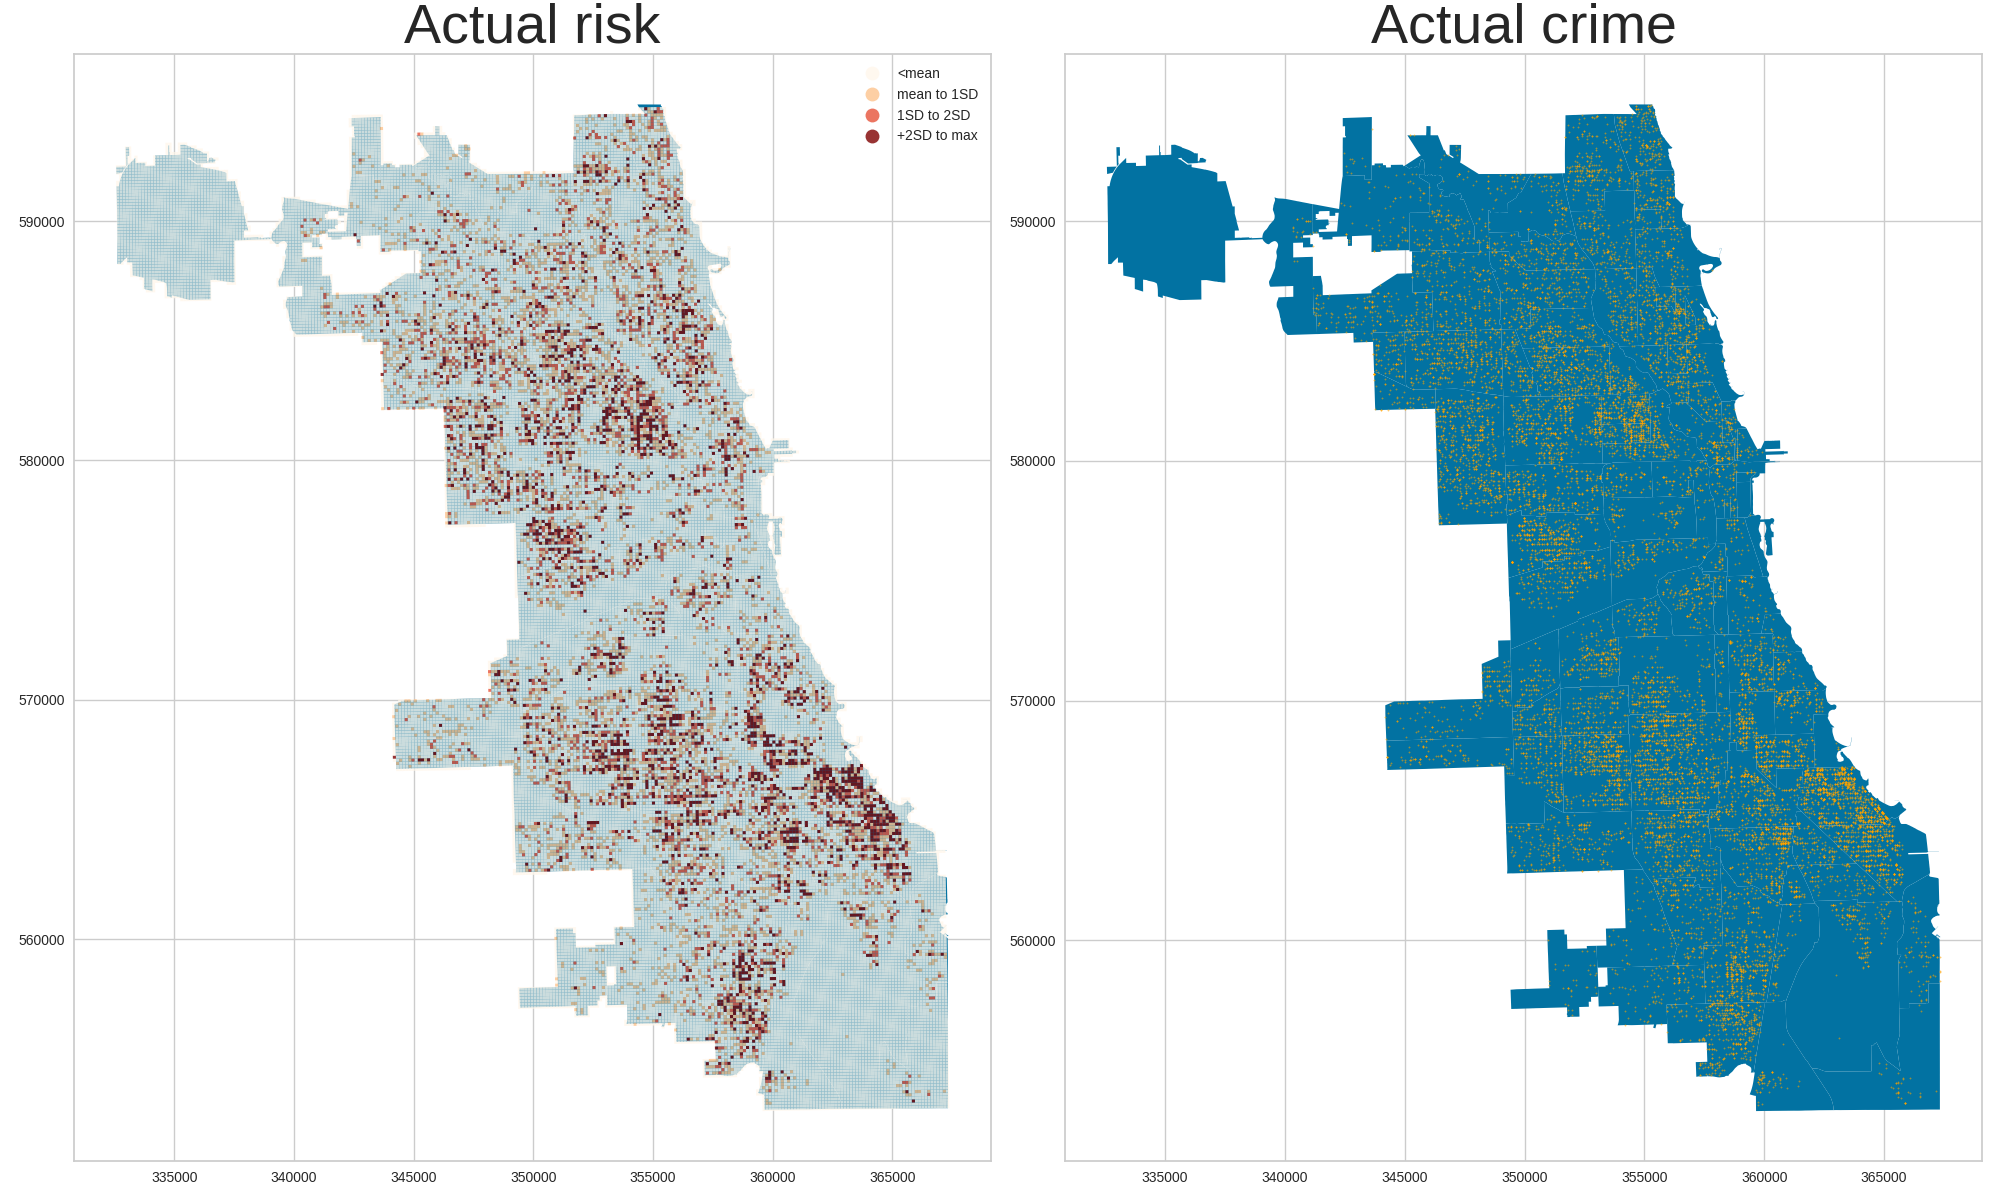
\includegraphics[scale=0.25]{./util-fig/actual_risk_point_map.png}
  \caption{左:実際のリスクマップ 右:実際の強盗犯罪発生地点}
  \label{fig:non-crime-timeseries-actual-risk}
\end{figure}

\begin{figure}
  \centering % 図を中央寄せにする
  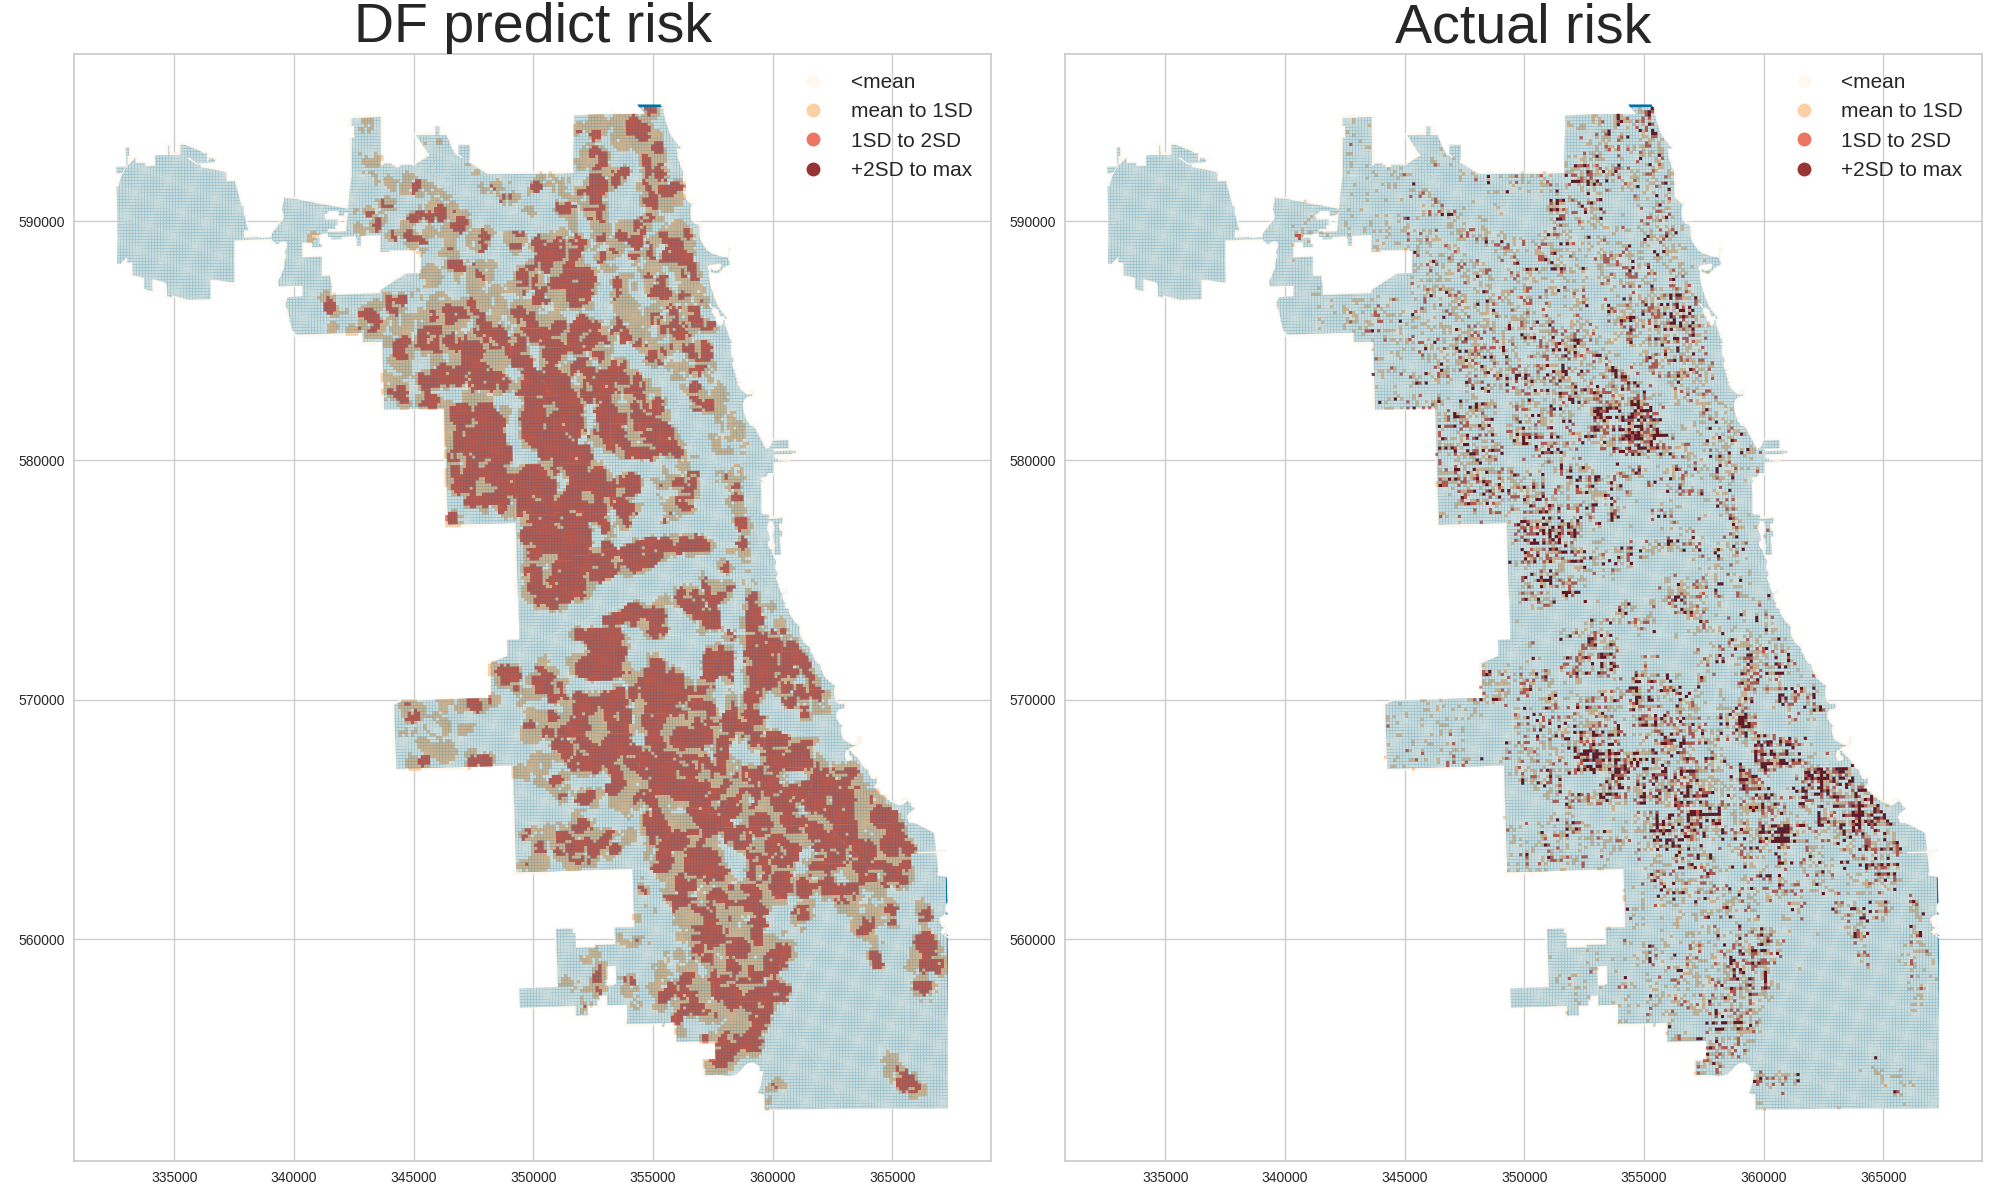
\includegraphics[scale=0.25]{./non-crime-timeseries-fig/DF_riskmap.png}
  \caption{左:DFによるリスクマップ 右:実際のリスクマップ}
  \label{fig:non-crime-timeseries-df-risk}
\end{figure}

\begin{figure}
  \centering % 図を中央寄せにする
  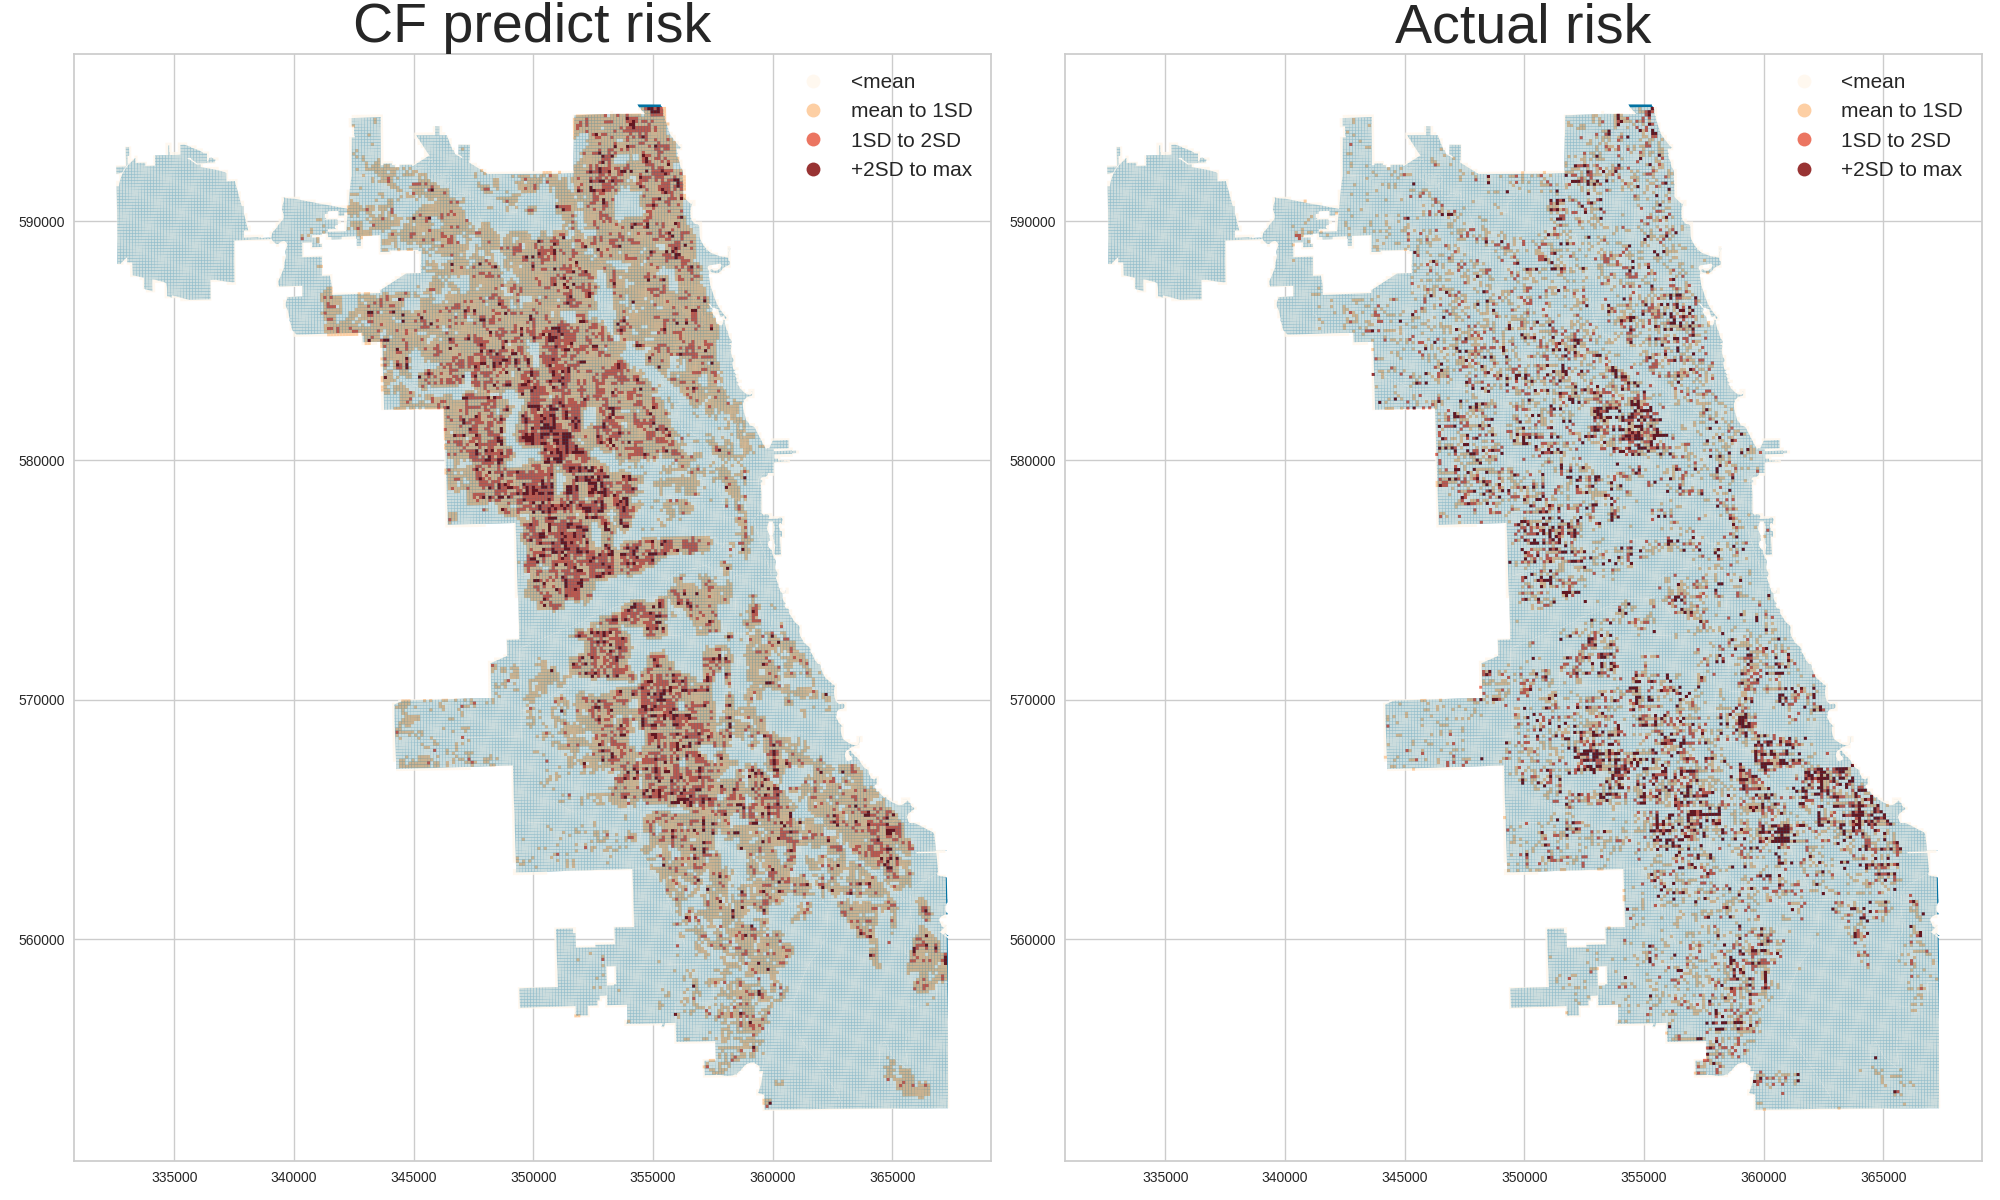
\includegraphics[scale=0.25]{./non-crime-timeseries-fig/CF_riskmap.png}
  \caption{左:CFによるリスクマップ 右:実際のリスクマップ}
  \label{fig:non-crime-timeseries-cf-risk}
\end{figure}

\begin{figure}
  \centering % 図を中央寄せにする
  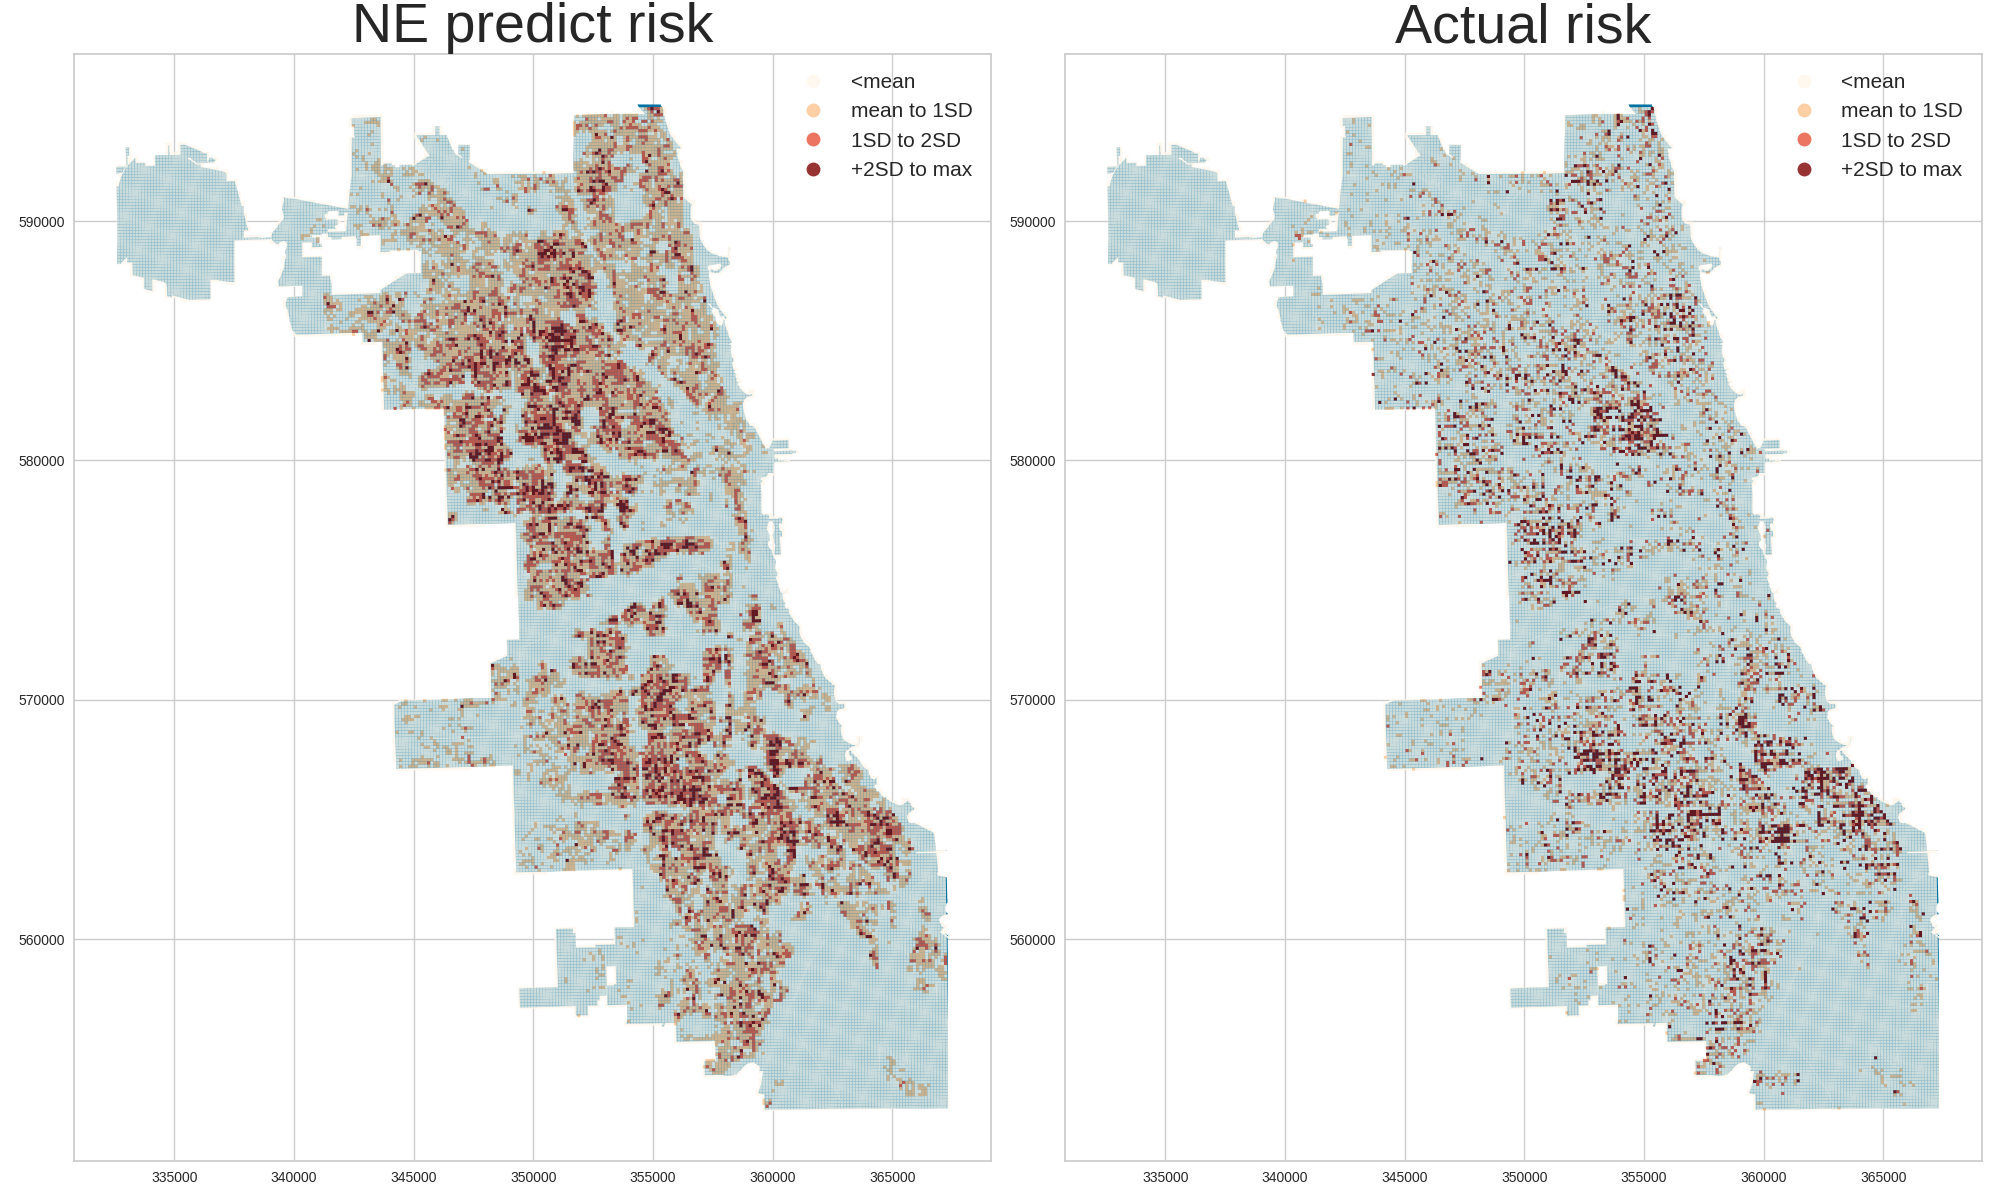
\includegraphics[scale=0.25]{./non-crime-timeseries-fig/NE_riskmap.png}
  \caption{左:NEによるリスクマップ 右:実際のリスクマップ}
  \label{fig:non-crime-timeseries-ne-risk}
\end{figure}

\begin{figure}
  \centering % 図を中央寄せにする
  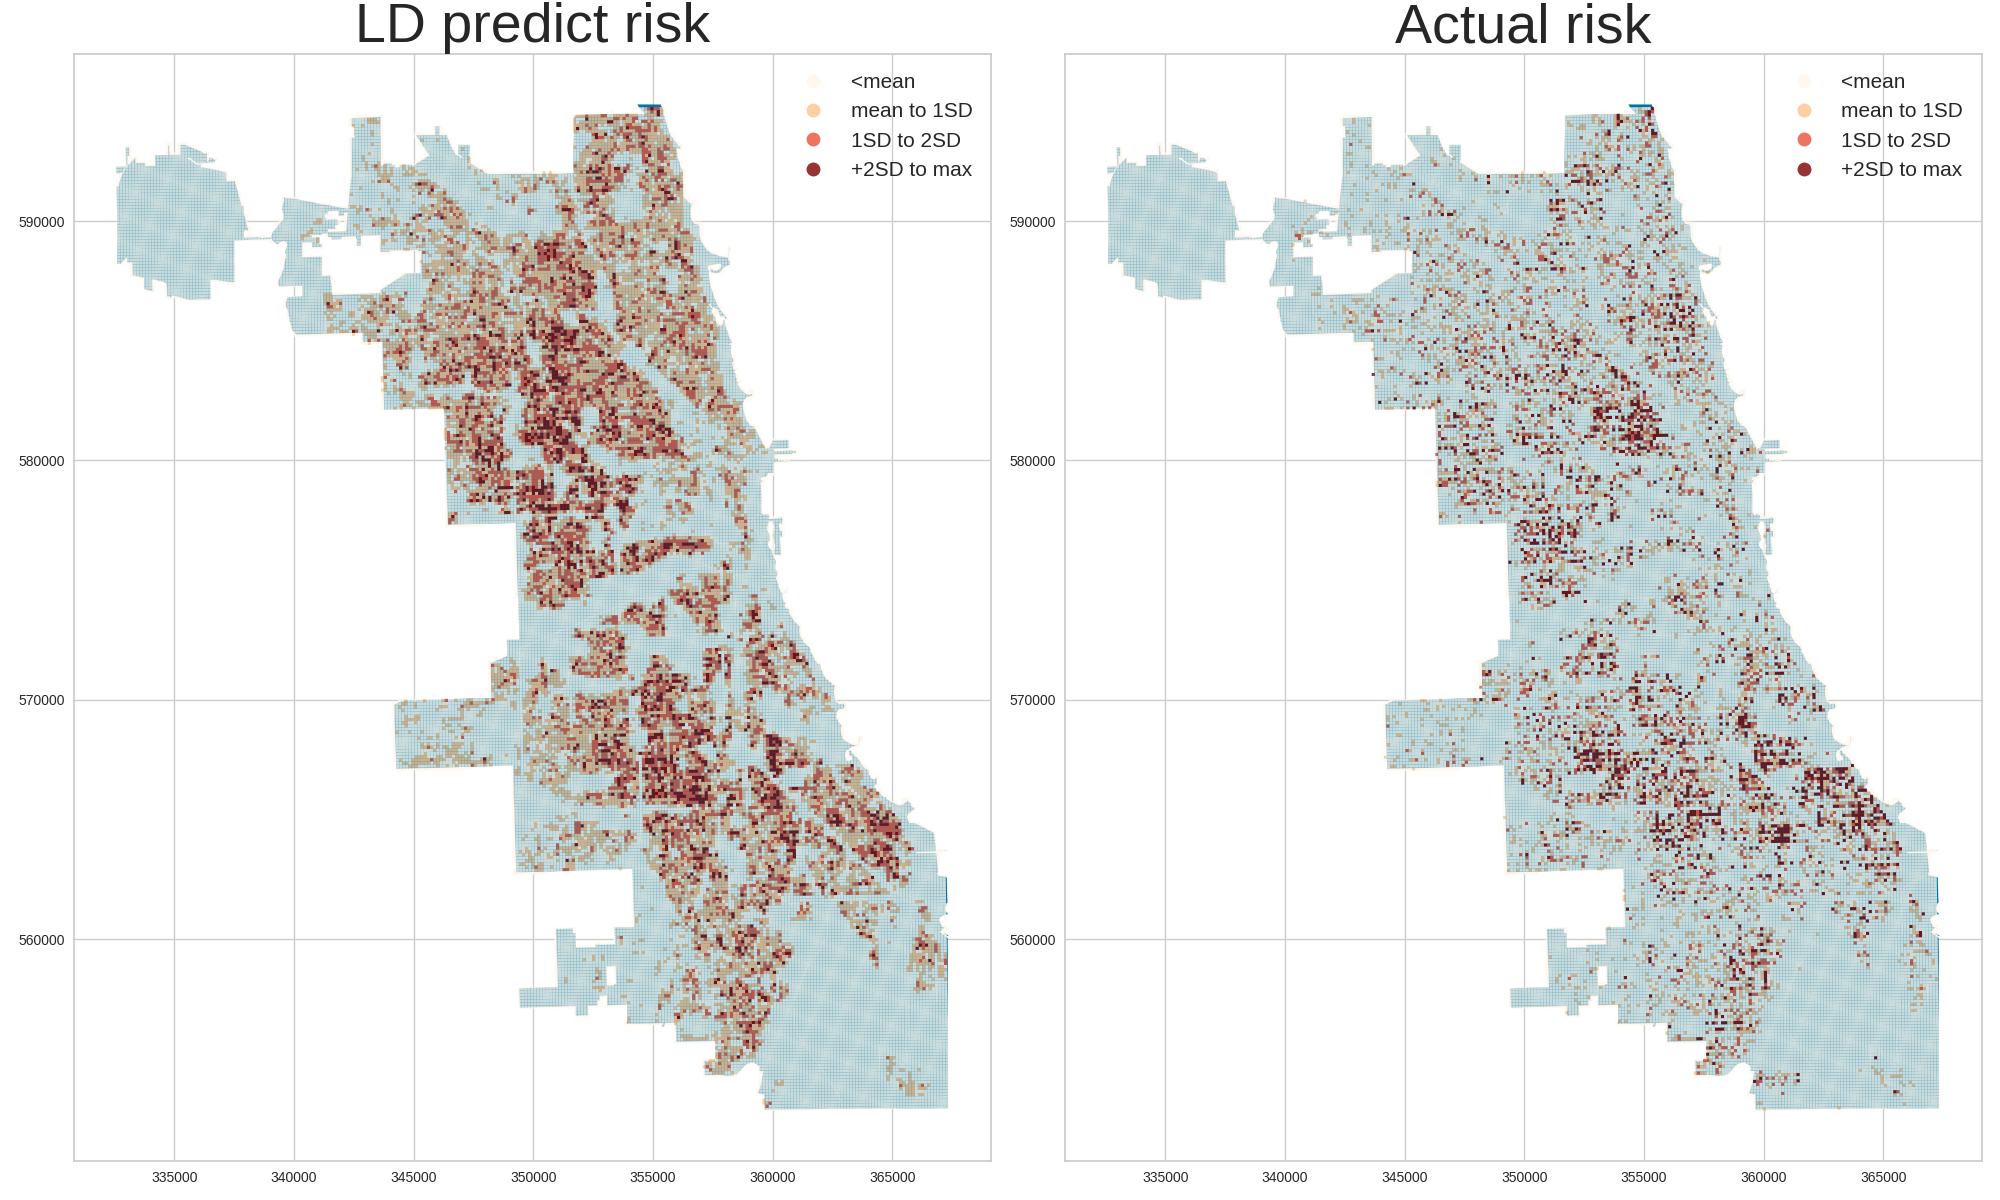
\includegraphics[scale=0.25]{./non-crime-timeseries-fig/LD_riskmap.png}
  \caption{左:LDによるリスクマップ 右:実際のリスクマップ}
  \label{fig:non-crime-timeseries-ld-risk}
\end{figure}

\begin{figure}
  \centering % 図を中央寄せにする
  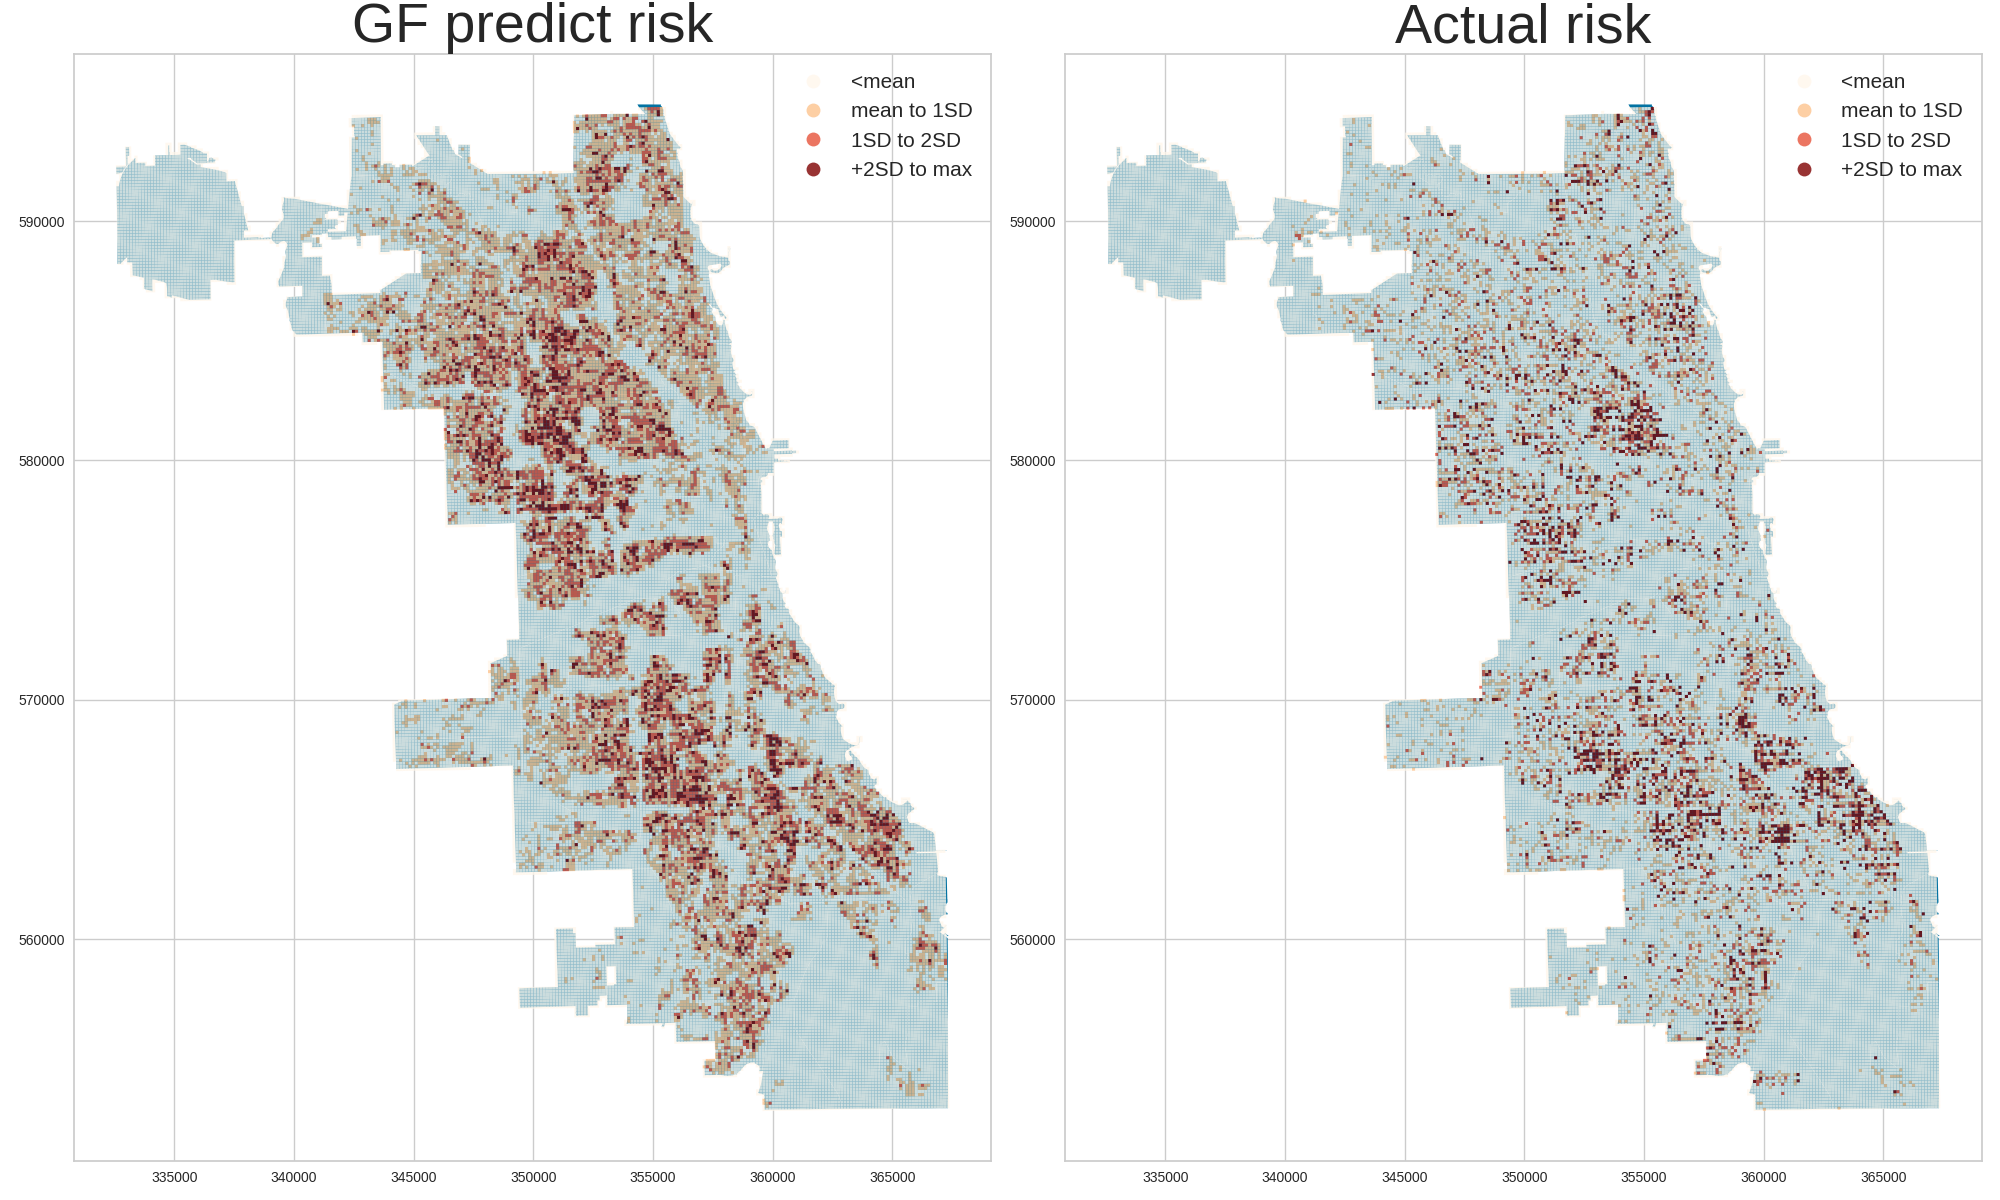
\includegraphics[scale=0.25]{./non-crime-timeseries-fig/GF_riskmap.png}
  \caption{左:GFによるリスクマップ 右:実際のリスクマップ}
  \label{fig:non-crime-timeseries-gf-risk}
\end{figure}

\begin{figure}
  \centering % 図を中央寄せにする
  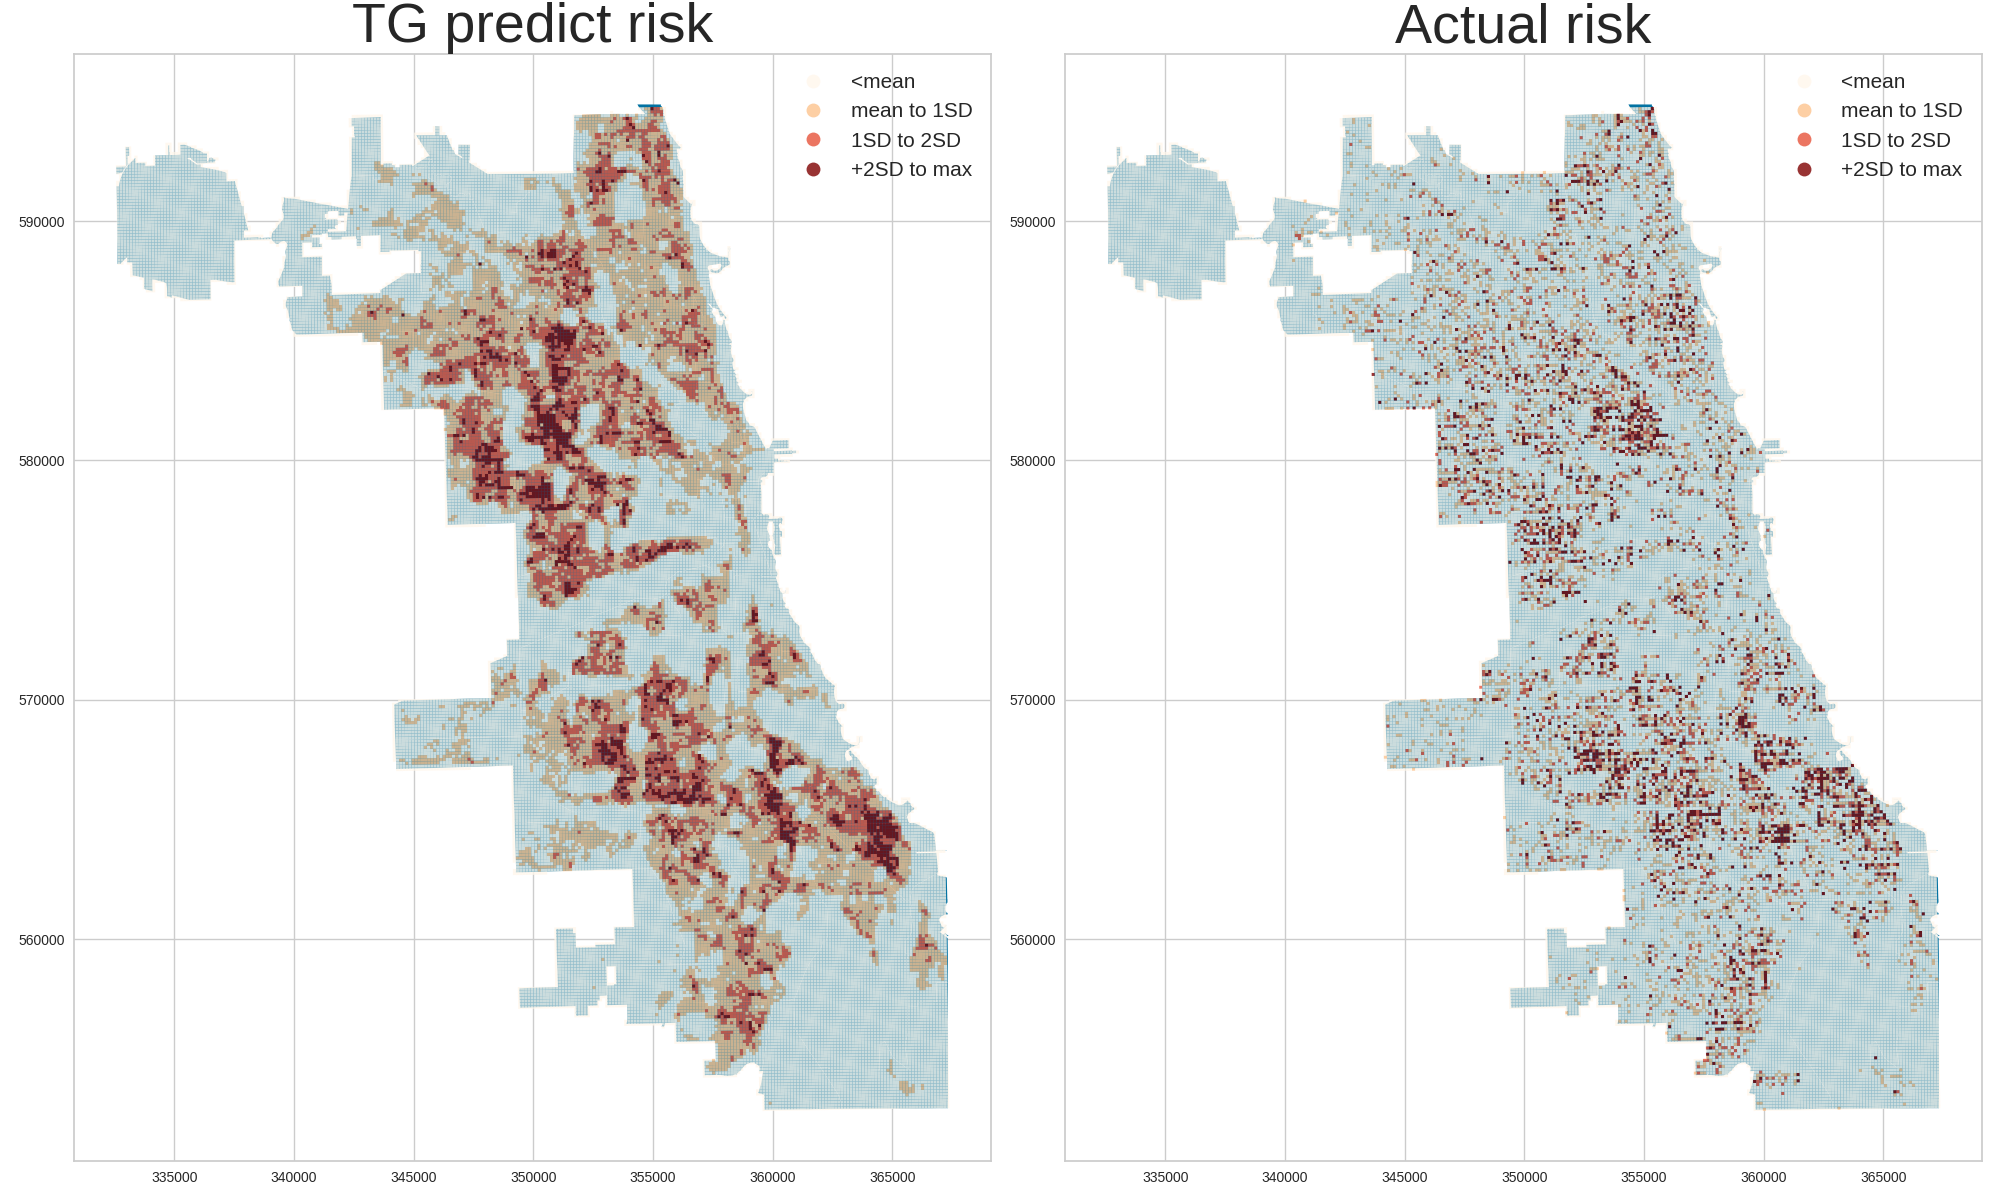
\includegraphics[scale=0.25]{./non-crime-timeseries-fig/TG_riskmap.png}
  \caption{左:TGによるリスクマップ 右:実際のリスクマップ}
  \label{fig:non-crime-timeseries-tg-risk}
\end{figure}

\begin{figure}
  \centering % 図を中央寄せにする
  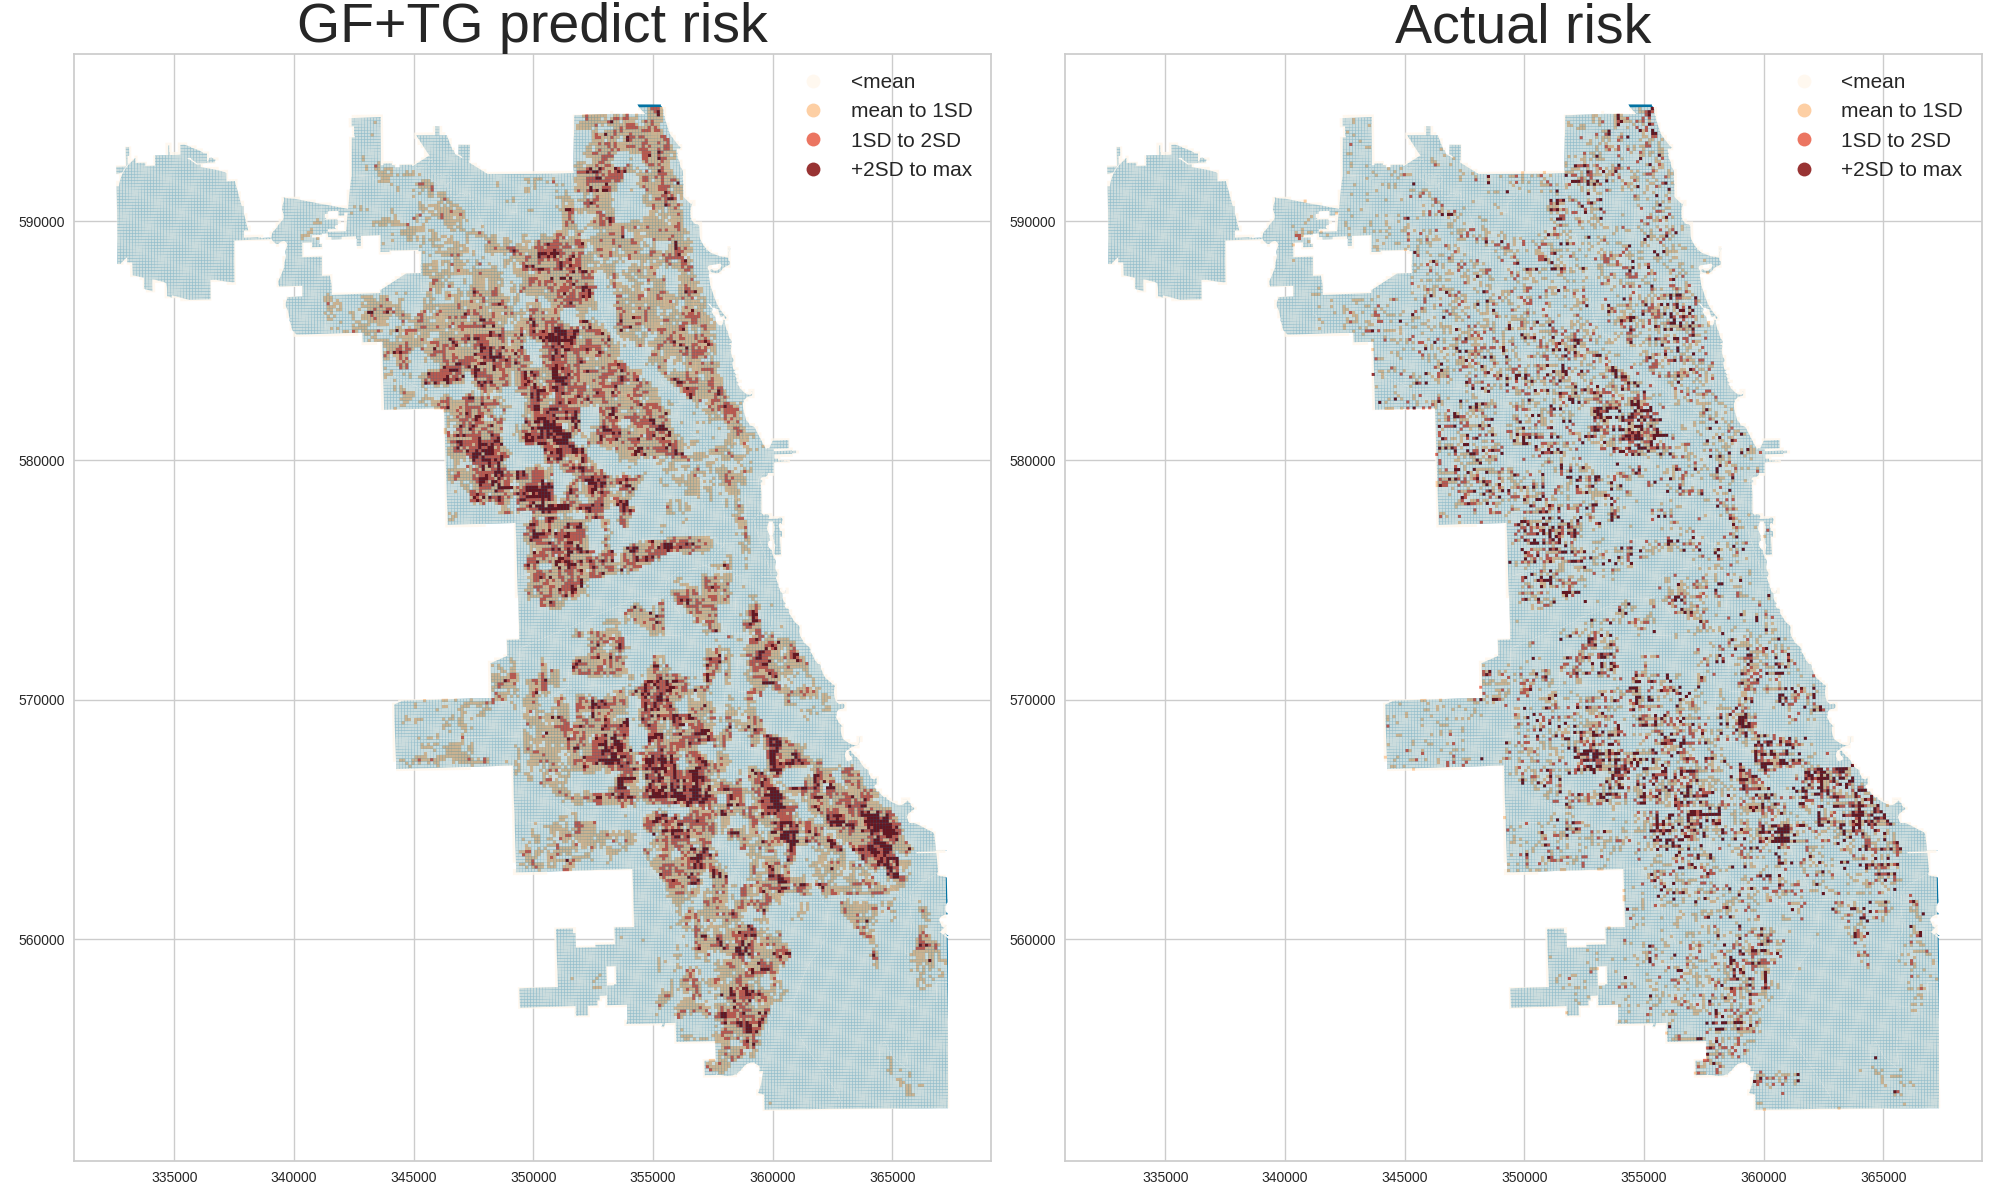
\includegraphics[scale=0.25]{./non-crime-timeseries-fig/GF+TG_riskmap.png}
  \caption{左:FG+TGによるリスクマップ 右:実際のリスクマップ}
  \label{fig:non-crime-timeseries-gf-tg-risk}
\end{figure}
%------------------------------------------
% confusion matrix
%------------------------------------------
\begin{figure}
  \centering % 図を中央寄せにする
  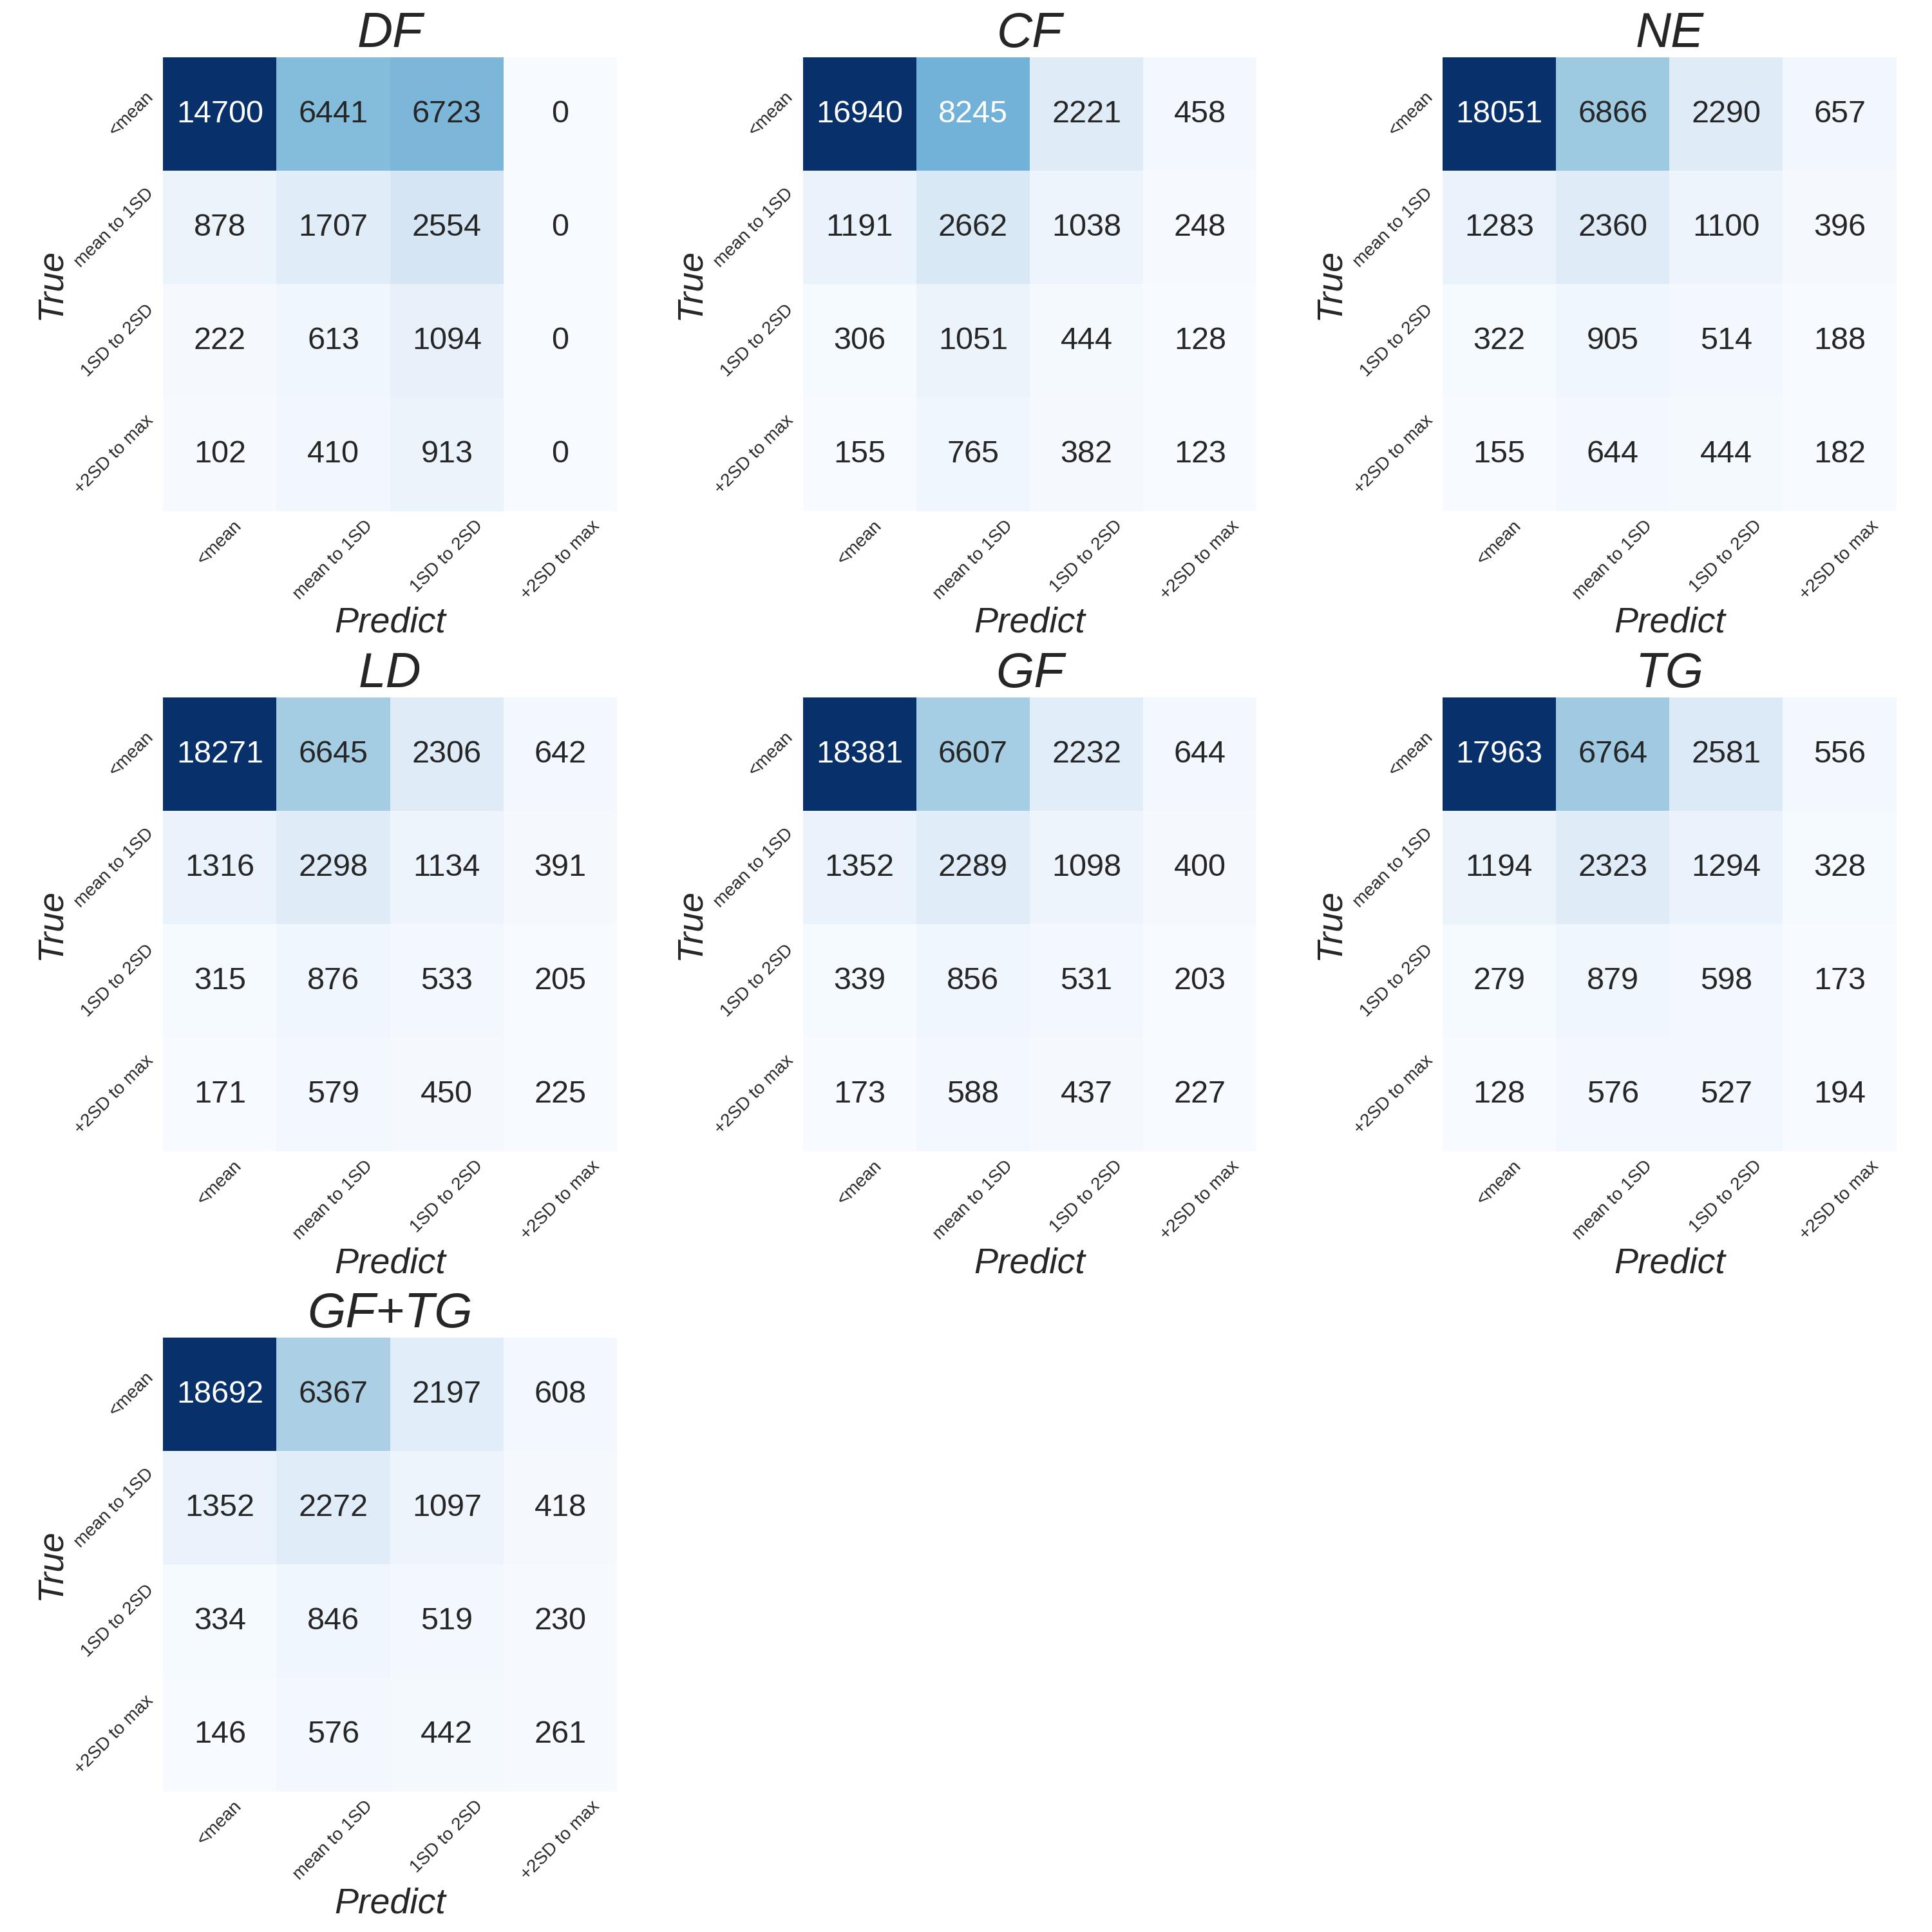
\includegraphics[scale=0.16]{./non-crime-timeseries-fig/non_crime_no_timeseries_four_cm.png}
  \caption{4カテゴリーの混同行列}
  \label{fig:non-crime-timeseries-4cm}
\end{figure}

\begin{figure}
  \centering % 図を中央寄せにする
  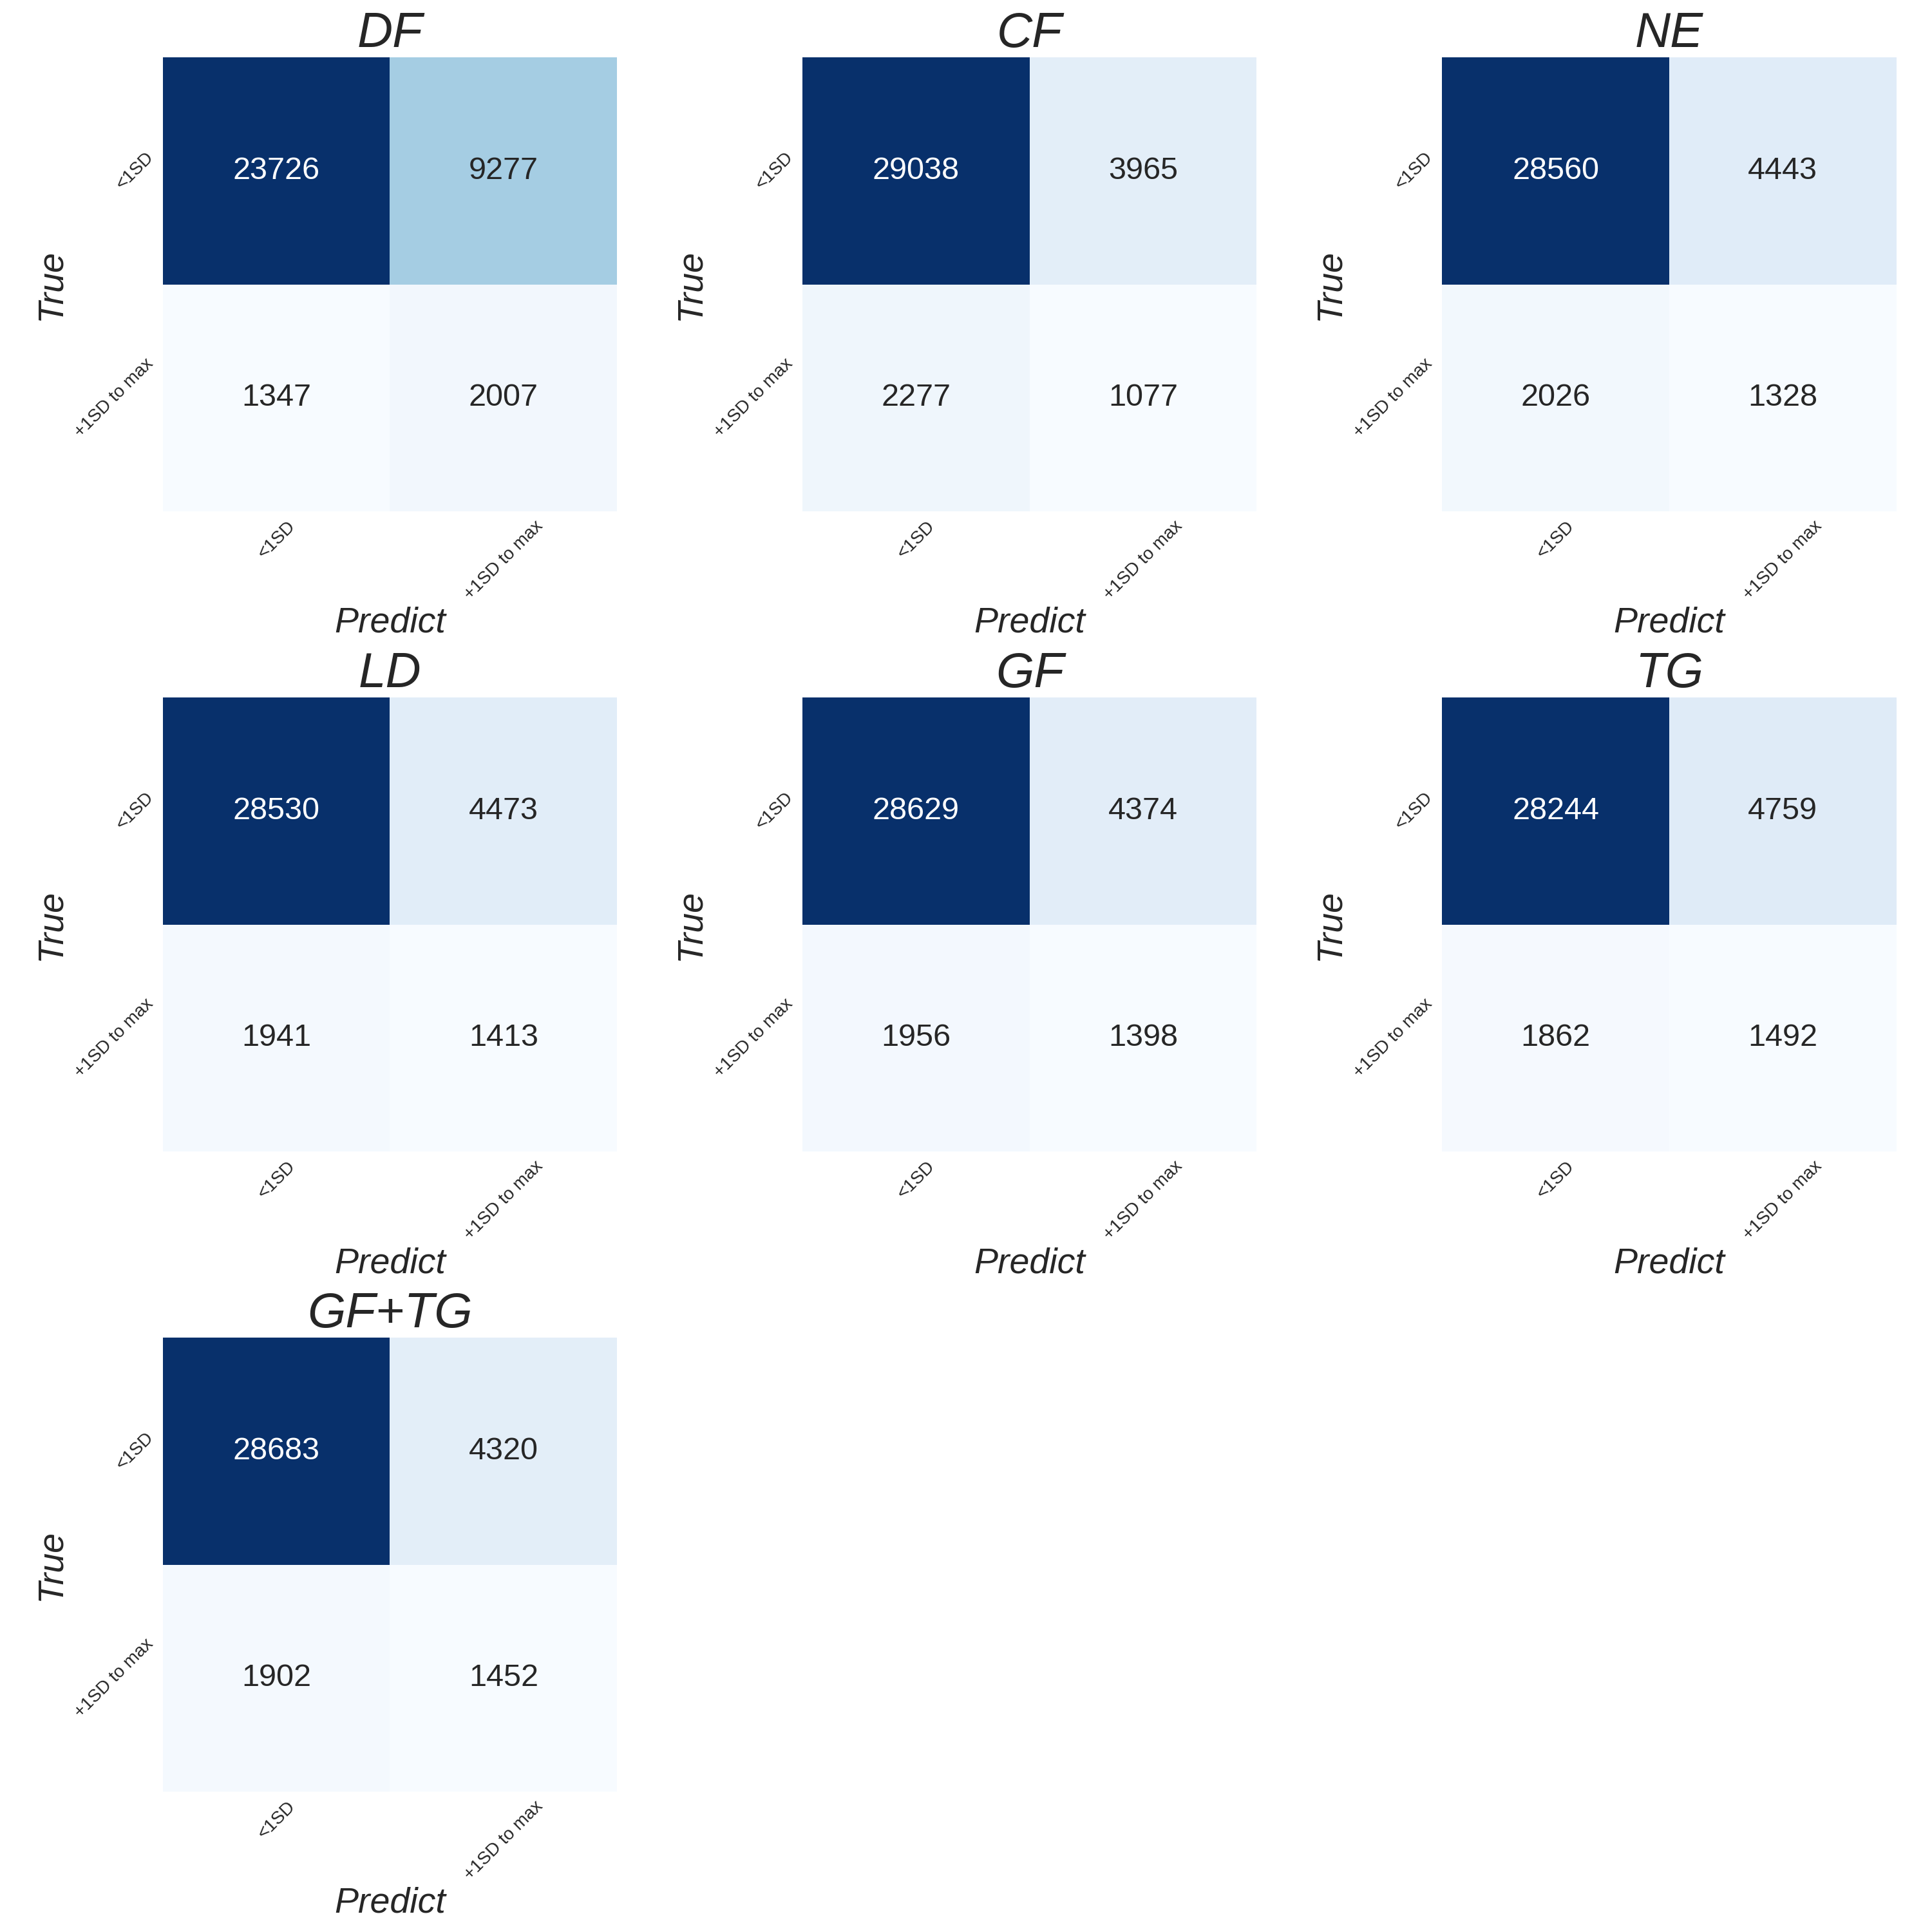
\includegraphics[scale=0.16]{./non-crime-timeseries-fig/non_crime_no_timeseries_two_cm.png}
  \caption{2カテゴリーの混同行列}
  \label{fig:non-crime-timeseries-2cm}
\end{figure}
% ---------------------------------
% FNFPplot
% ---------------------------------
\begin{figure}
  \centering % 図を中央寄せにする
  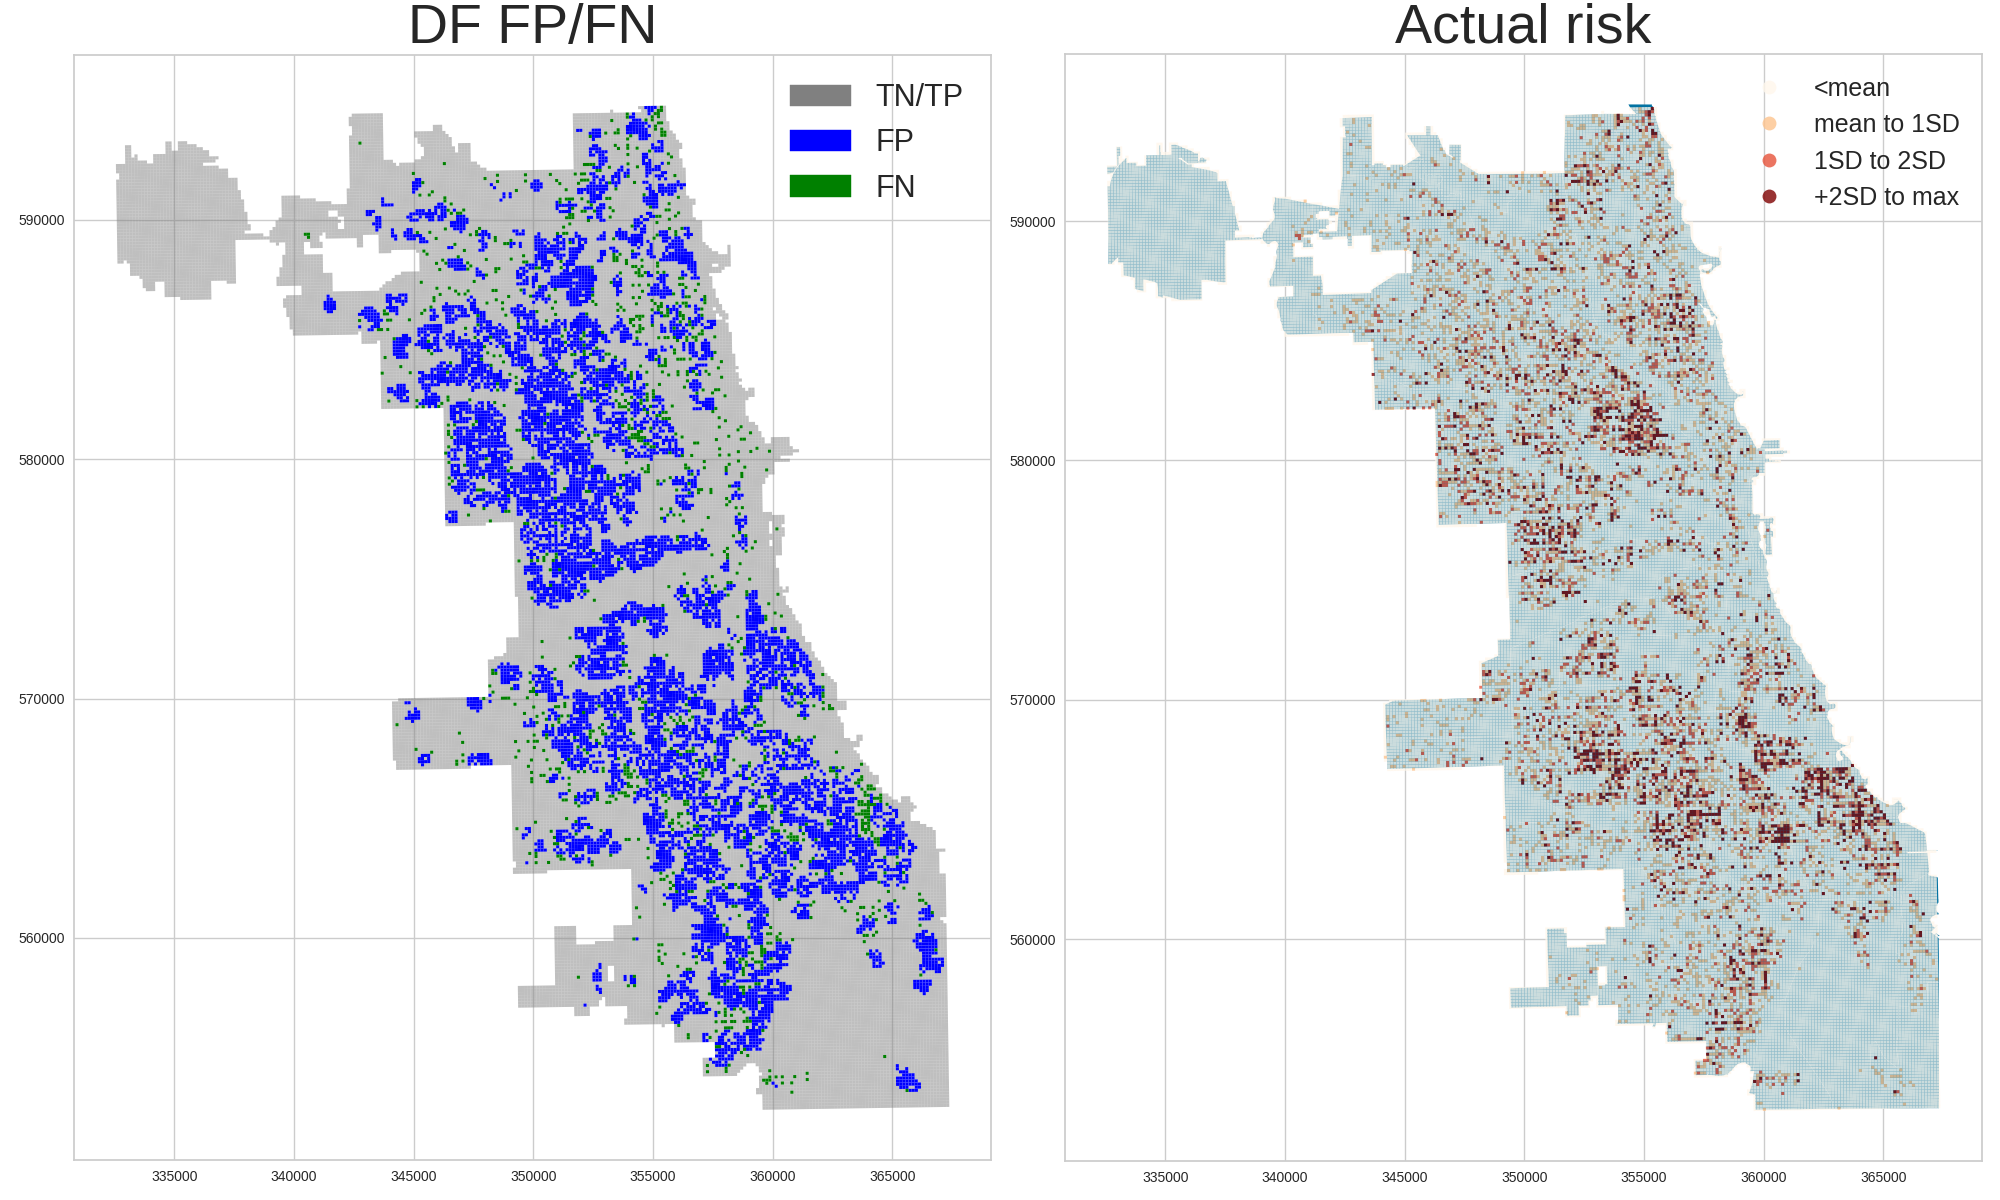
\includegraphics[scale=0.25]{./non-crime-timeseries-fig/DF_fnp.png}
  \caption{左:DFのFPFN 右:実際のリスクマップ}
  \label{fig:non-crime-timeseries-df-fnp}
\end{figure}

\begin{figure}
  \centering % 図を中央寄せにする
  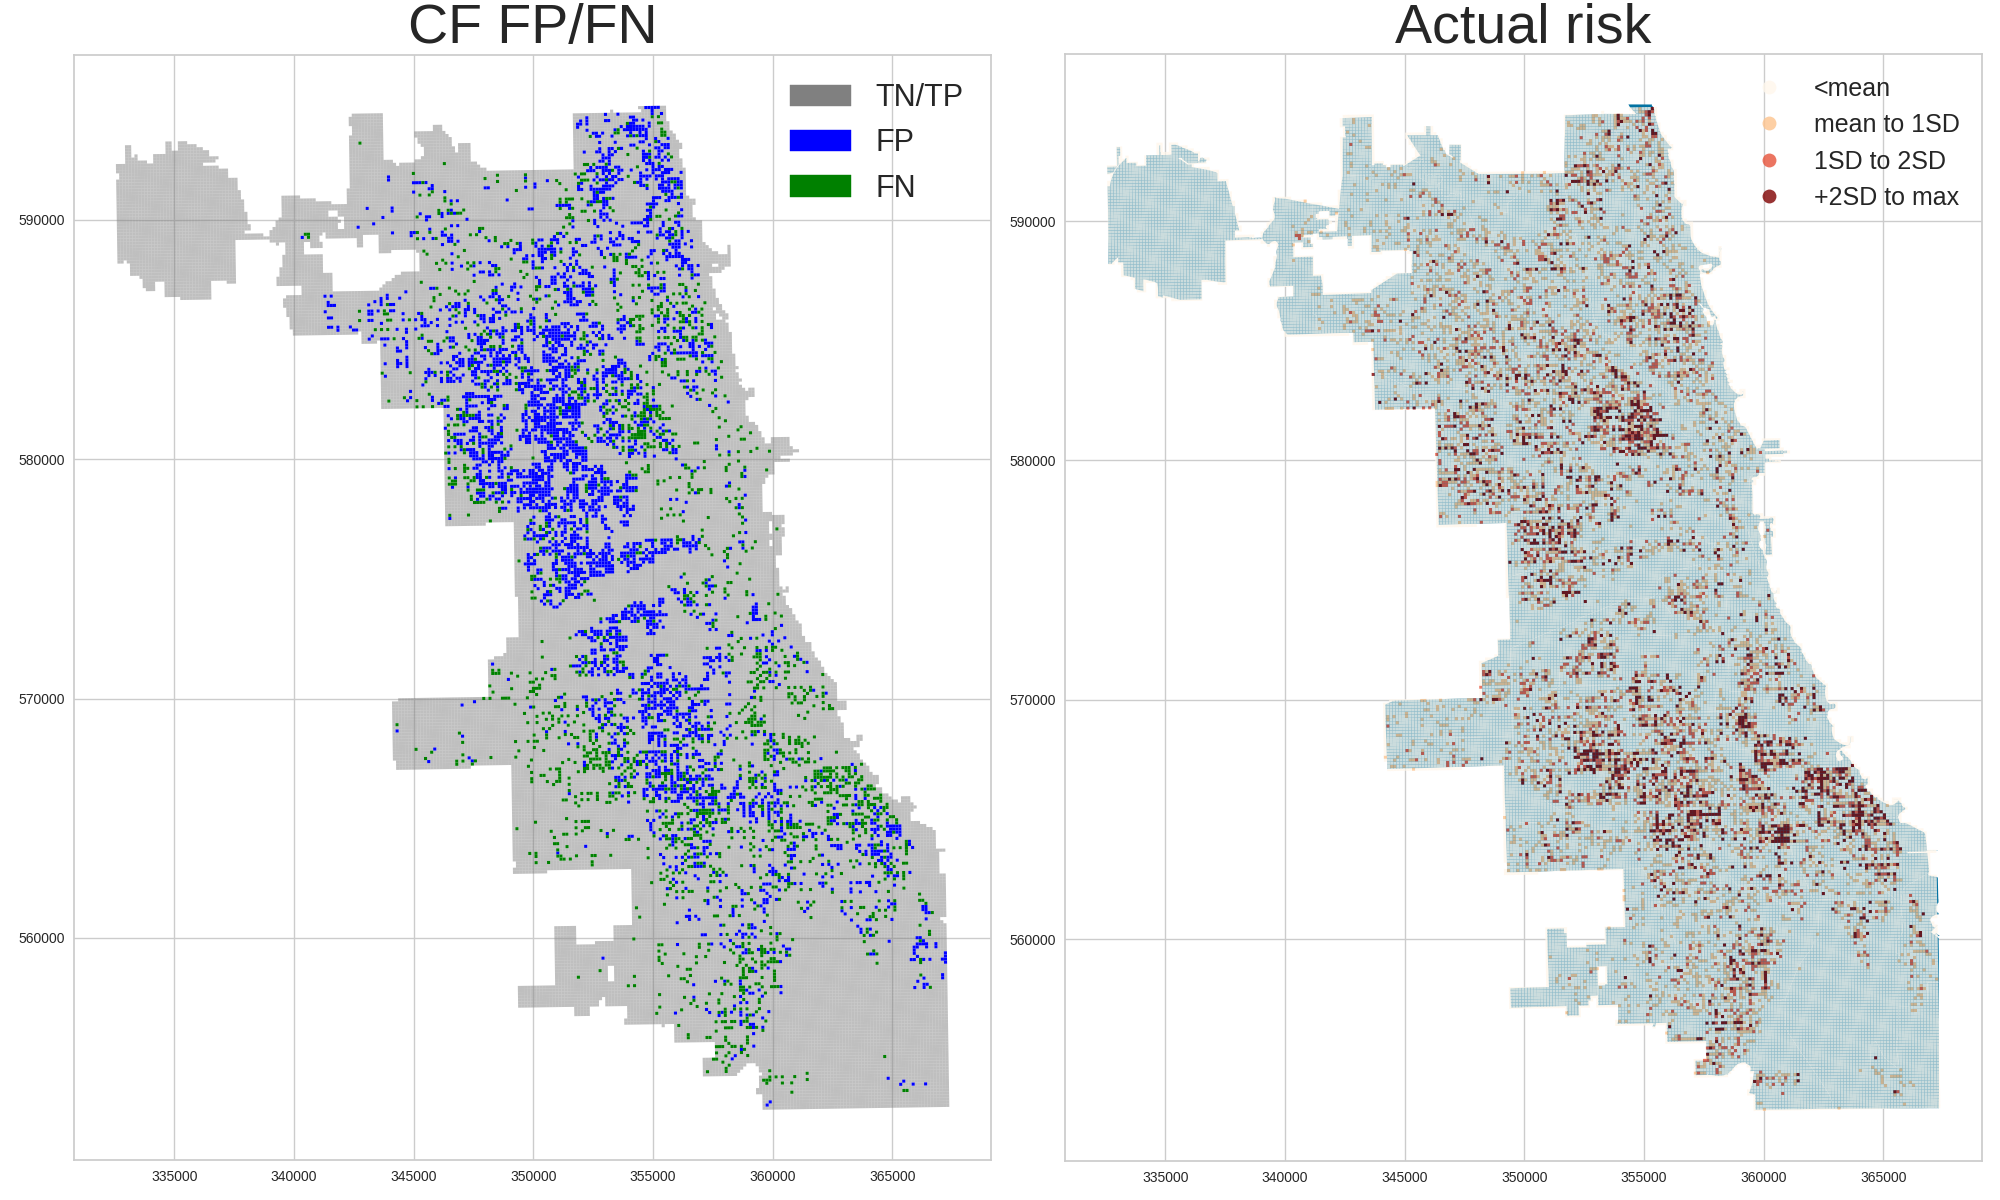
\includegraphics[scale=0.25]{./non-crime-timeseries-fig/CF_fnp.png}
  \caption{左:CFのFPFN 右:実際のリスクマップ}
  \label{fig:non-crime-timeseries-cf-fnp}
\end{figure}

\begin{figure}
  \centering % 図を中央寄せにする
  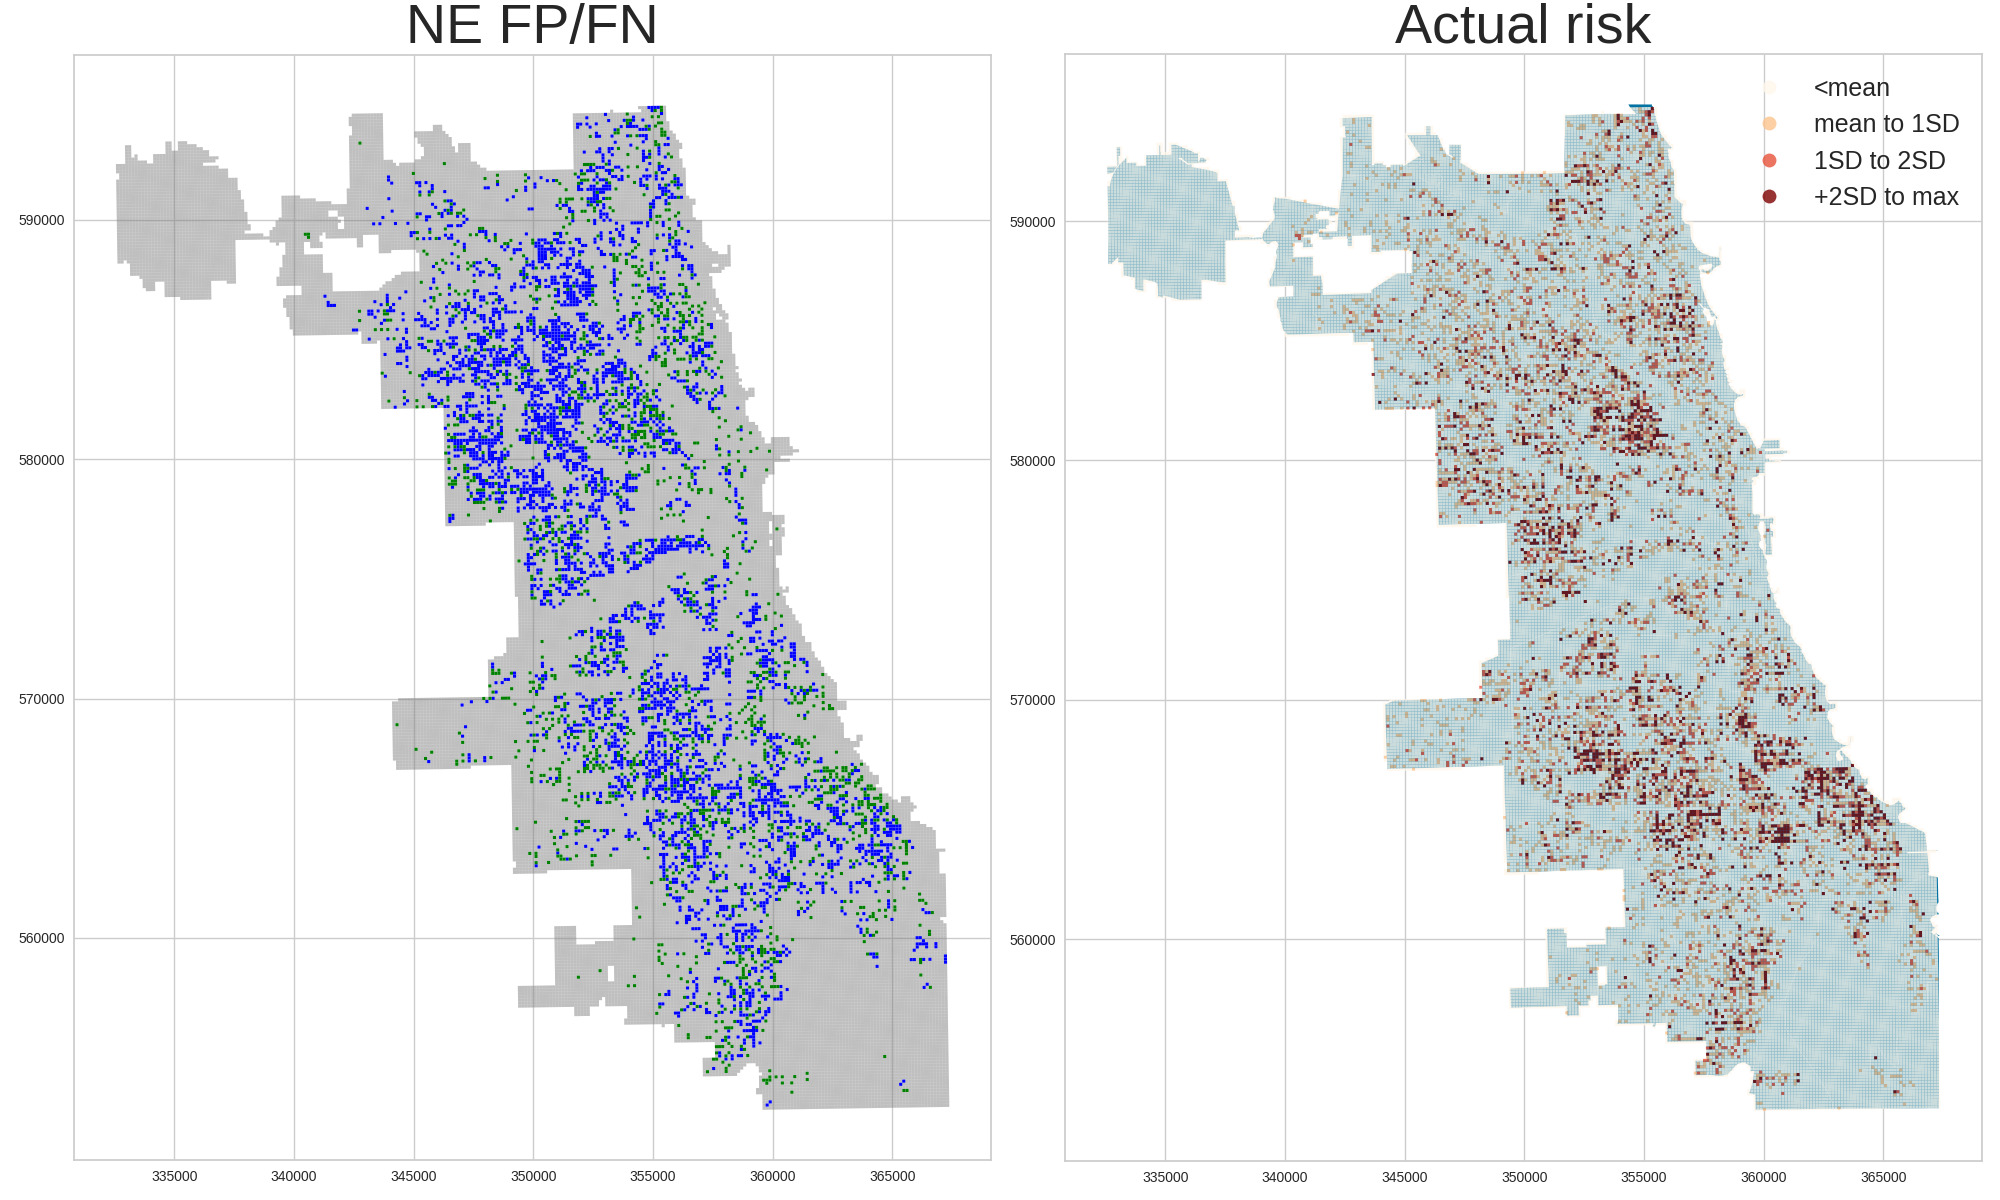
\includegraphics[scale=0.25]{./non-crime-timeseries-fig/NE_fnp.png}
  \caption{左:NEのFPFN 右:実際のリスクマップ}
  \label{fig:non-crime-timeseries-ne-fnp}
\end{figure}

\begin{figure}
  \centering % 図を中央寄せにする
  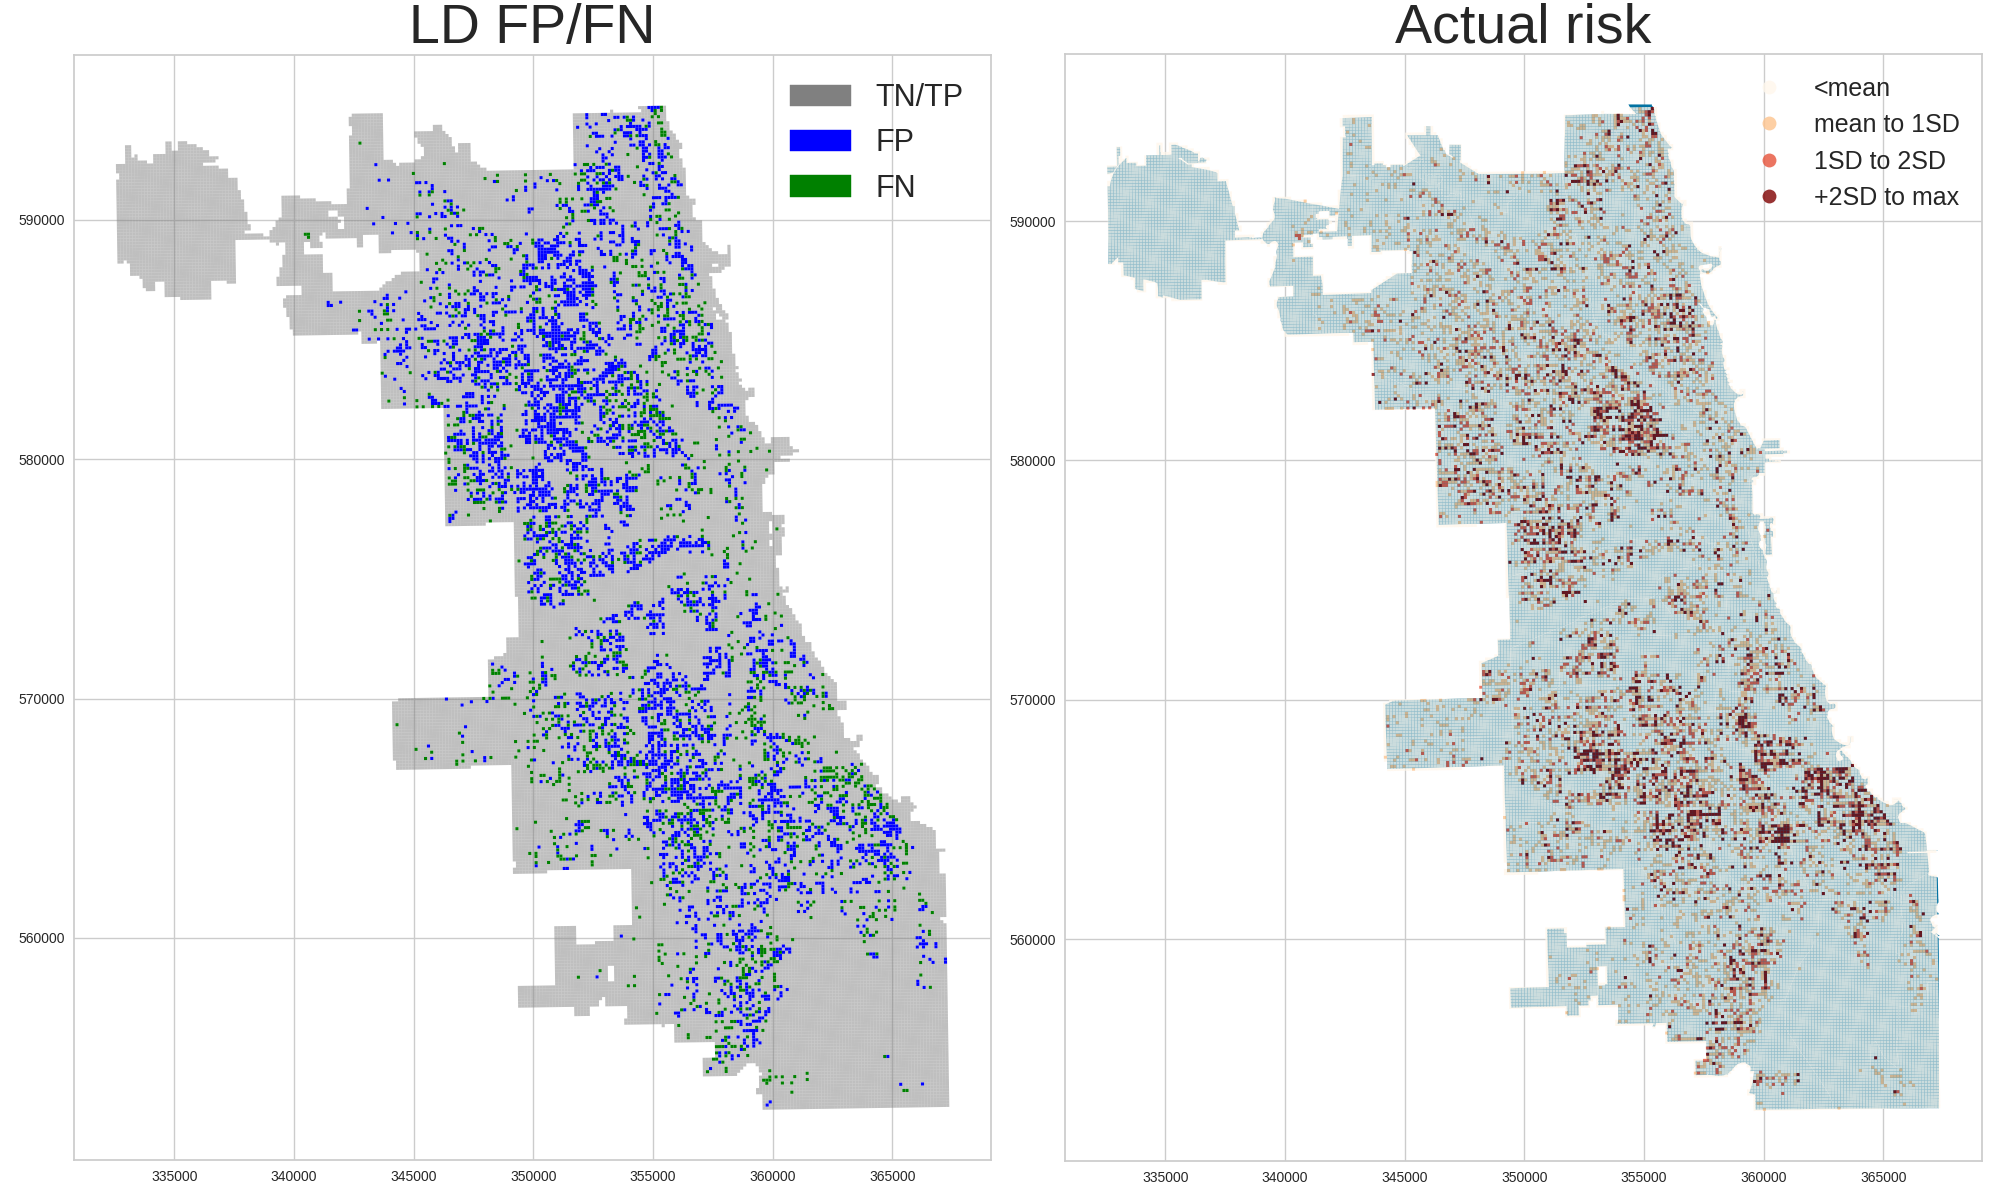
\includegraphics[scale=0.25]{./non-crime-timeseries-fig/LD_fnp.png}
  \caption{左:LDのFPFN 右:実際のリスクマップ}
  \label{fig:non-crime-timeseries-ld-fnp}
\end{figure}

\begin{figure}
  \centering % 図を中央寄せにする
  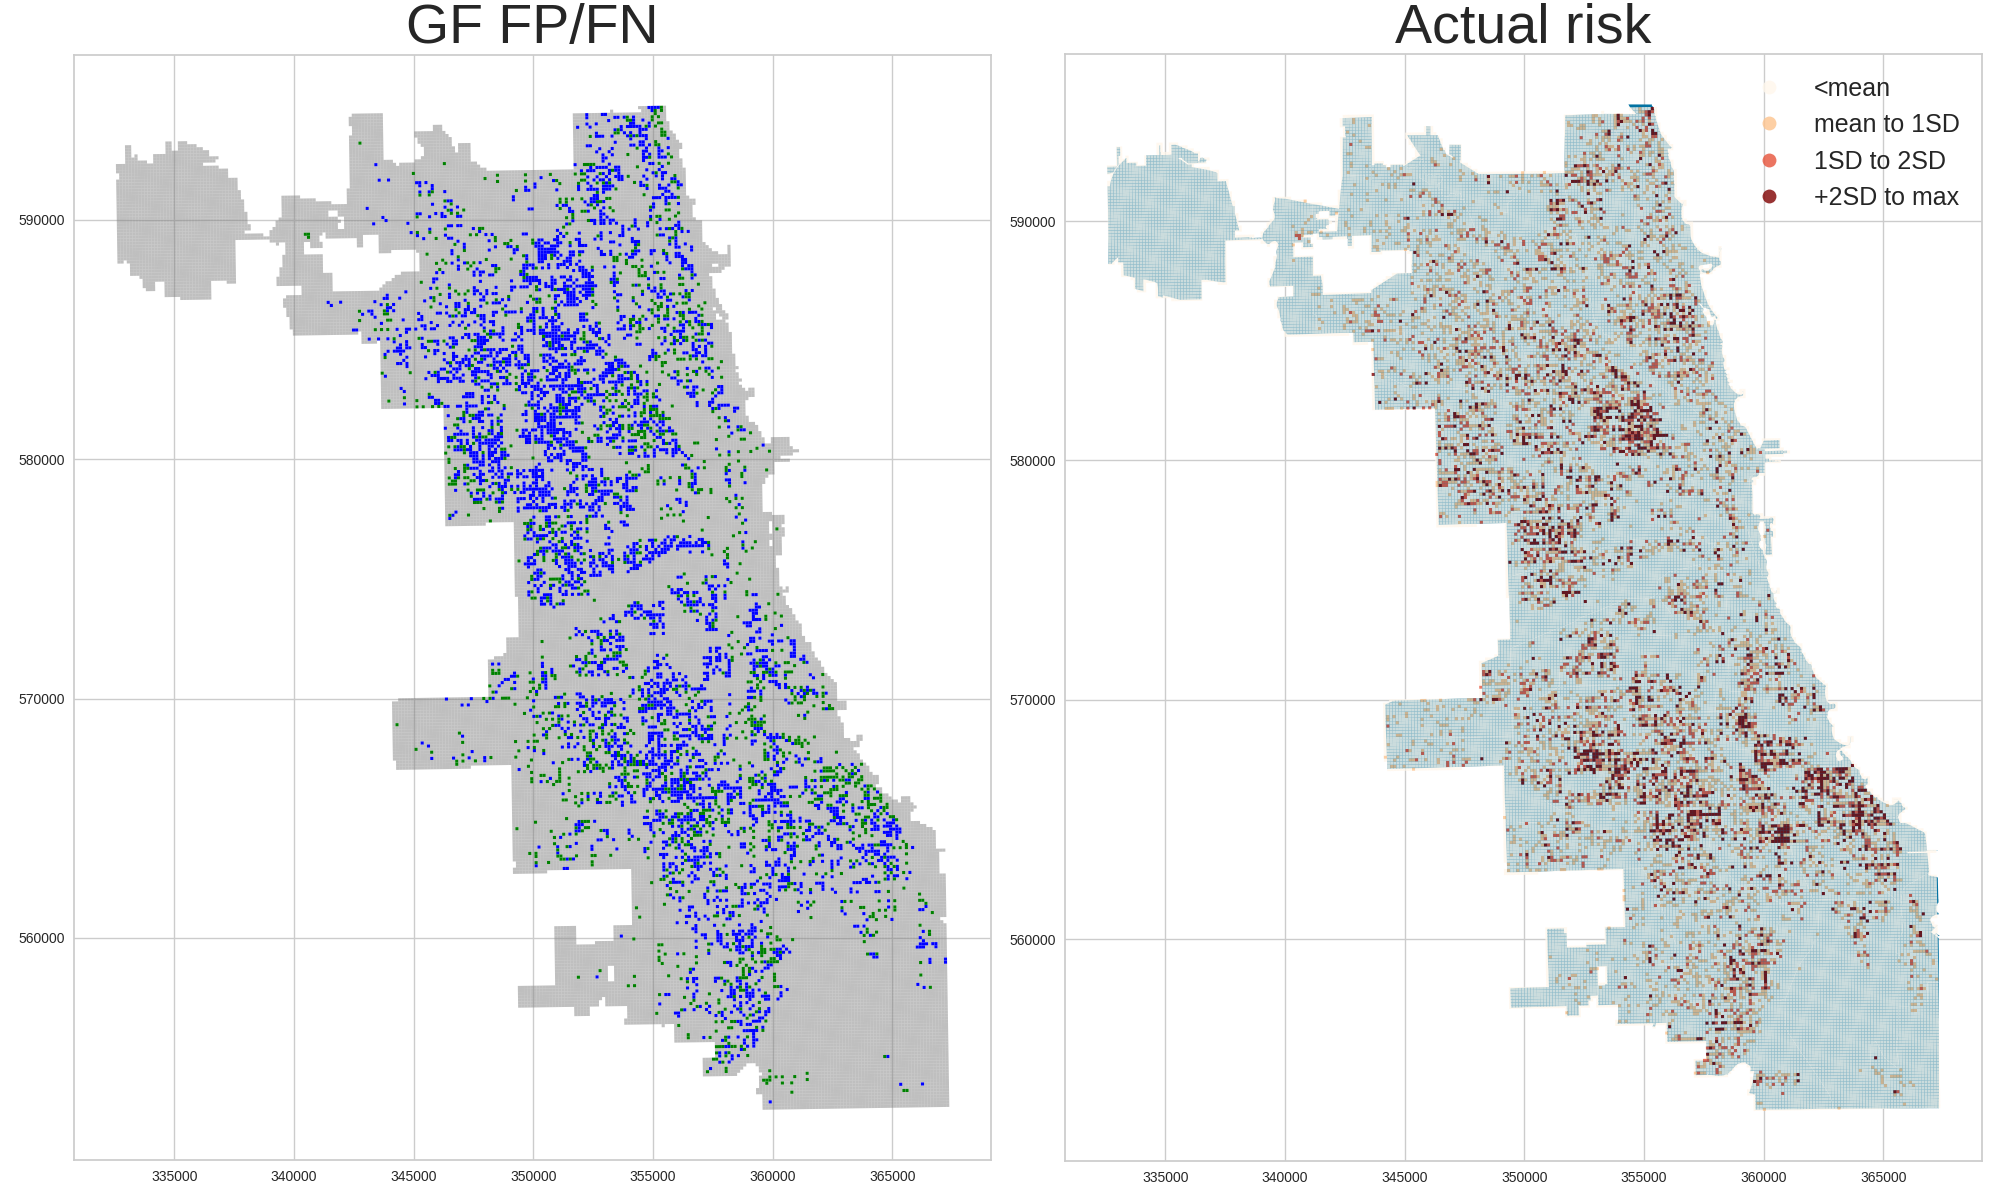
\includegraphics[scale=0.25]{./non-crime-timeseries-fig/GF_fnp.png}
  \caption{左:GFのFPFN 右:実際のリスクマップ}
  \label{fig:non-crime-timeseries-gf-fnp}
\end{figure}

\begin{figure}
  \centering % 図を中央寄せにする
  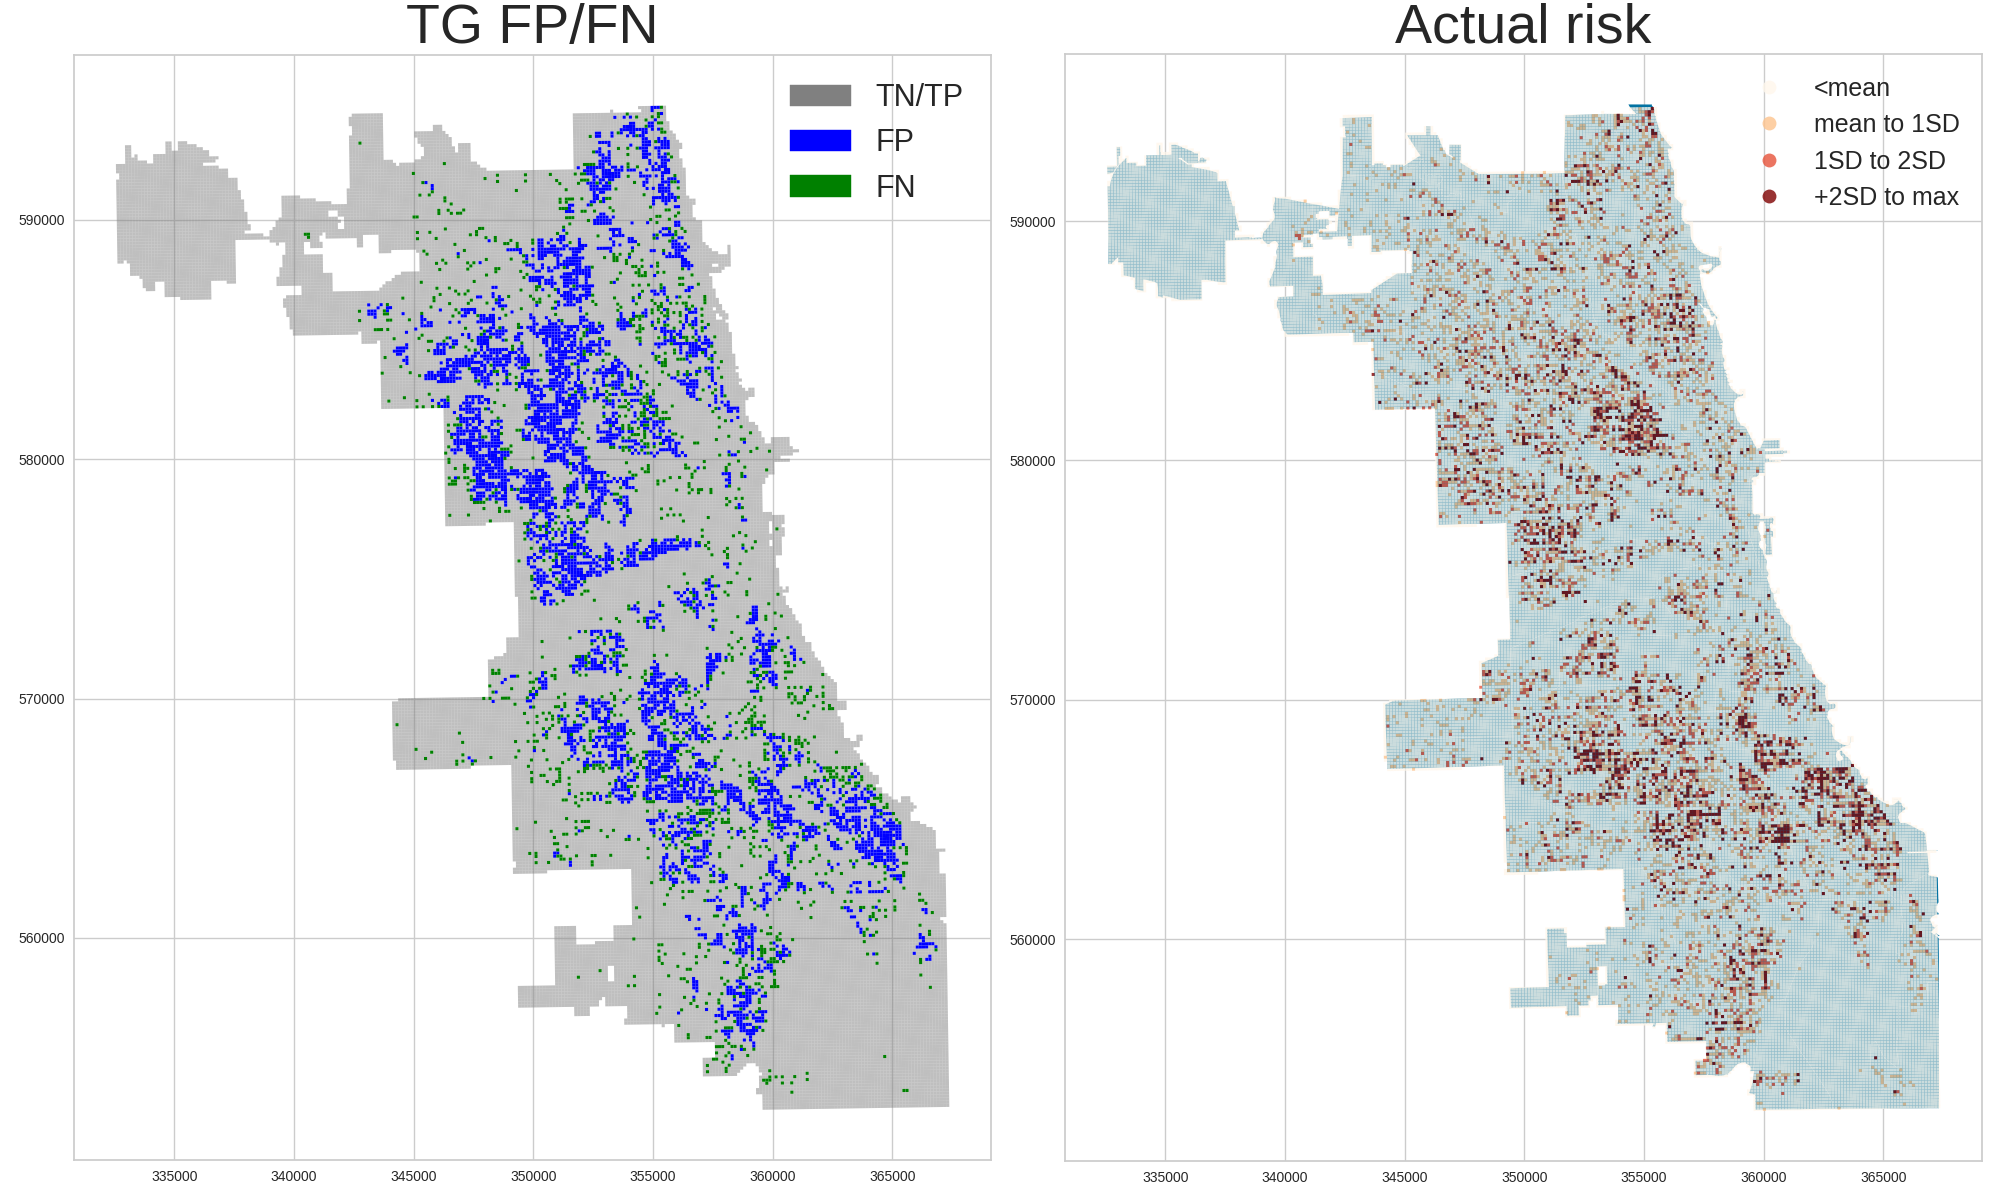
\includegraphics[scale=0.25]{./non-crime-timeseries-fig/TG_fnp.png}
  \caption{左:TGのFPFN 右:実際のリスクマップ}
  \label{fig:non-crime-timeseries-tg-fnp}
\end{figure}

\begin{figure}
  \centering % 図を中央寄せにする
  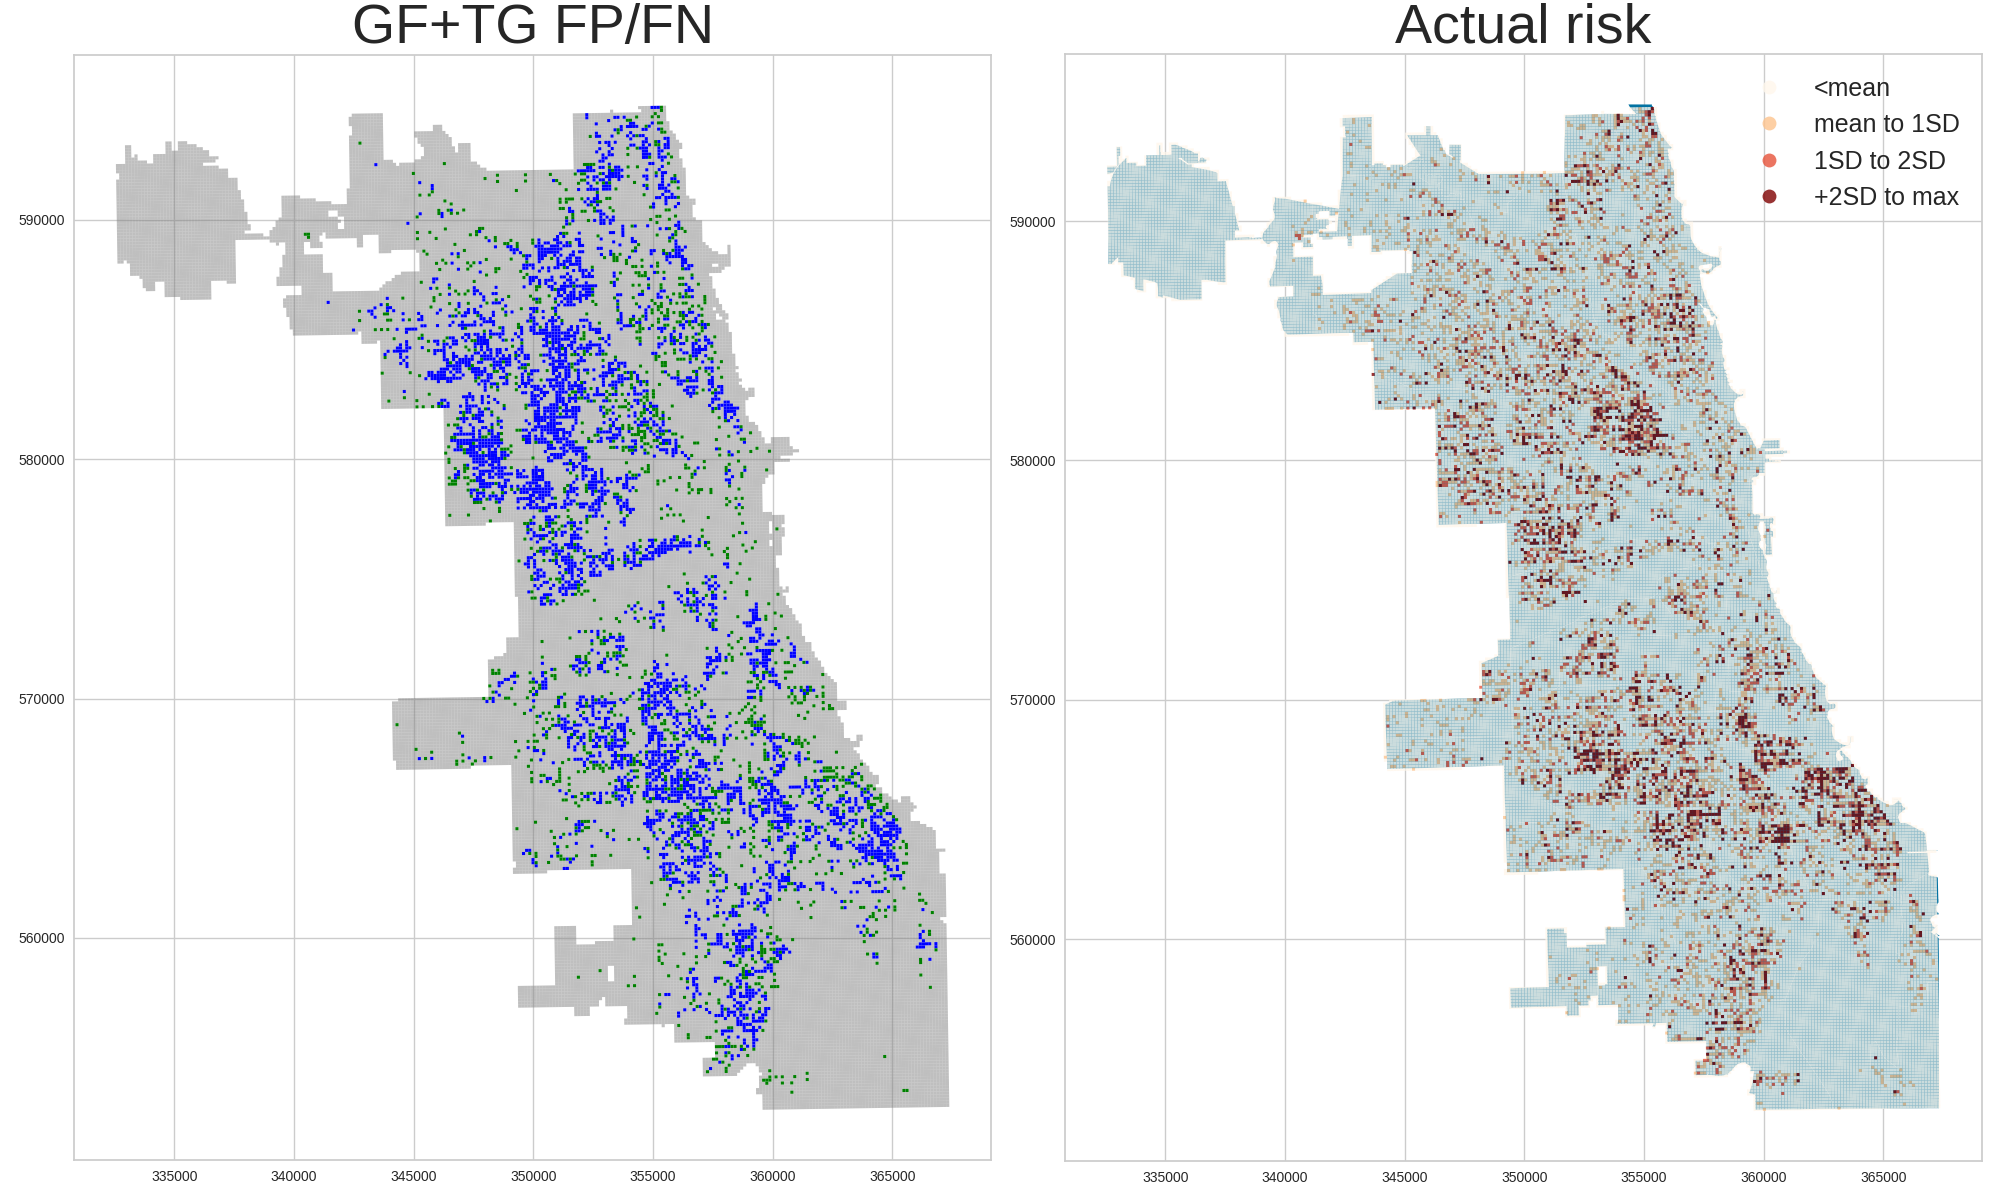
\includegraphics[scale=0.25]{./non-crime-timeseries-fig/GF+TG_fnp.png}
  \caption{左:GF+TGのFPFN 右:実際のリスクマップ}
  \label{fig:non-crime-timeseries-gf-tg-fnp}
\end{figure}
%------------------------------------------
% ROC curve
%------------------------------------------
また,各モデルのROC曲線を図\ref{fig:non-crime-timeseries-roc}に示した.

\begin{figure}
  \centering % 図を中央寄せにする
  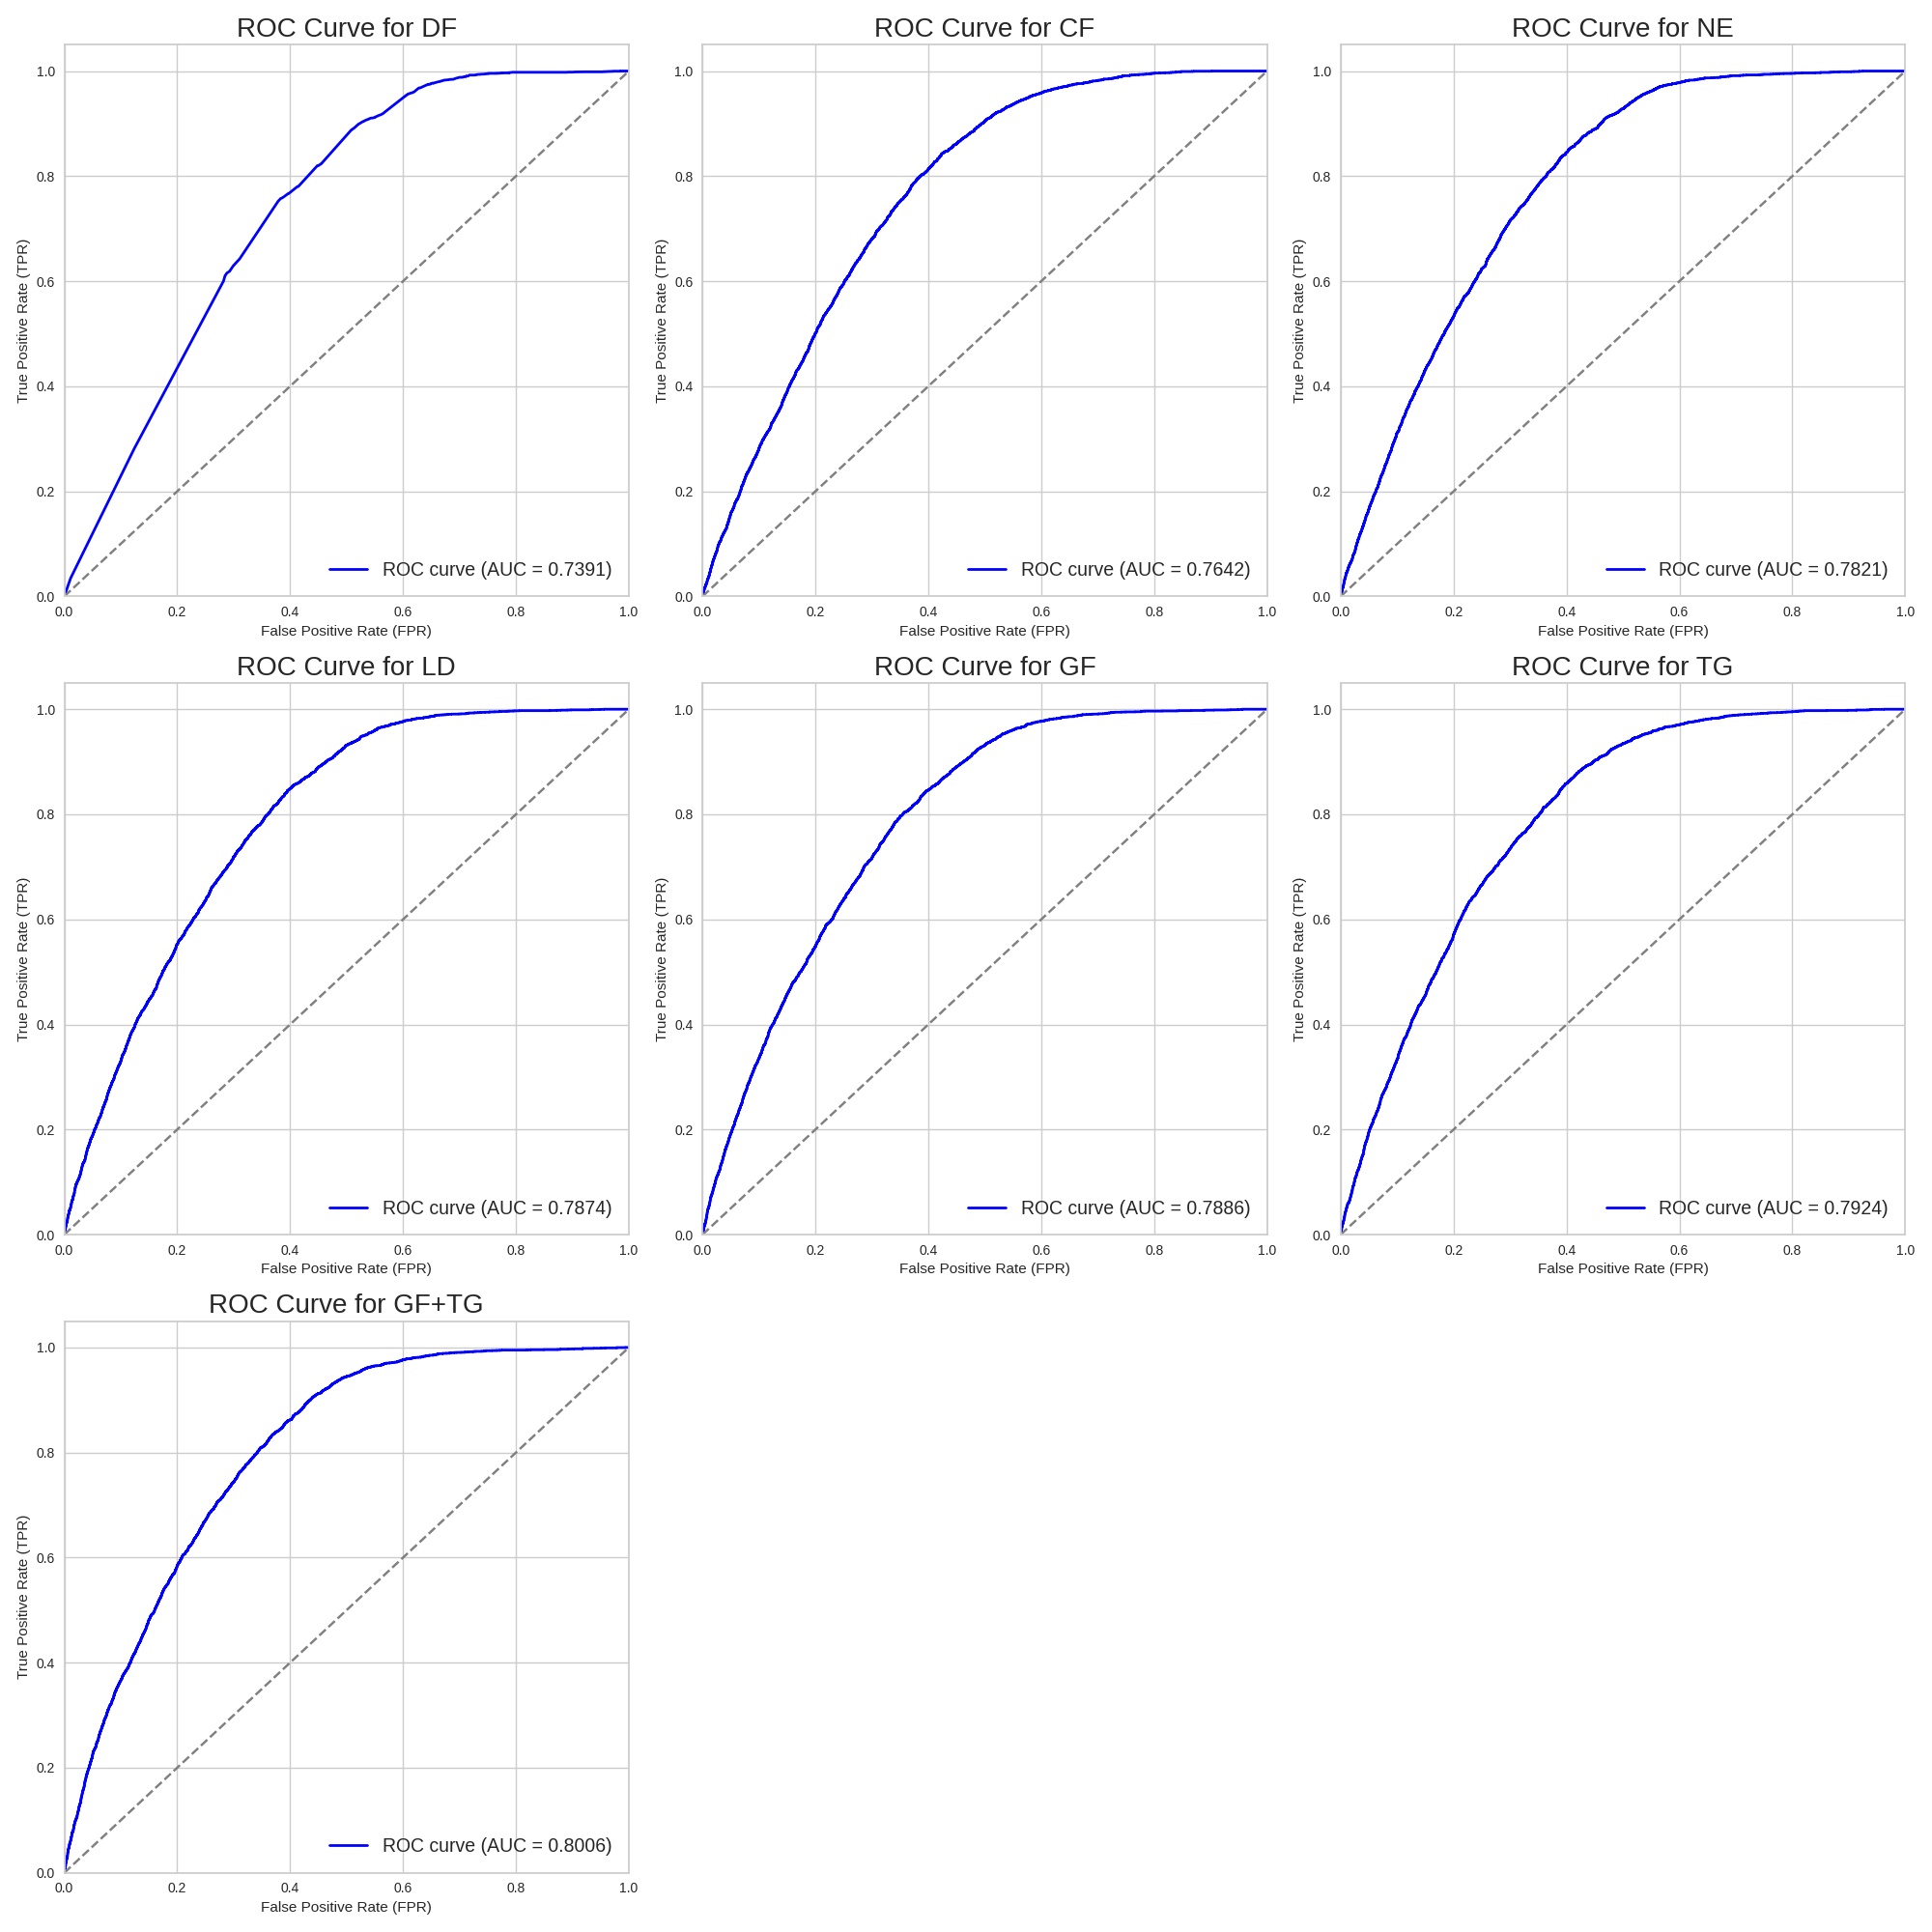
\includegraphics[scale=0.25]{./non-crime-timeseries-fig/roc_auc.png}
  \caption{ROC曲線}
  \label{fig:non-crime-timeseries-roc}
\end{figure}
%------------------------------------------
% table
%------------------------------------------
各モデルの予測精度を精度指標を基に比較した結果を表\ref{tb:fig:non-crime-timeseries-index}にまとめる.

\begin{table}[htbp]
  \centering
  \caption{各モデル間の精度比較}
  \begin{tabular}{l|r|r|r|r|r|r|r}
  \hline

  モデル & DF & CF & NE & LD & GF & TG & GF+TG \\  \hline\hline
  的中率 & 57.2 & 30.2 & 36.9 & 38.9 & 38.4 & 41.4 & 40.0 \\ 
  PAI & 1.84 & 2.18 & 2.33 & 2.40 & 2.42 & 2.41 & 2.52 \\ 
  AUC & 0.74 & 0.76 & 0.78 & 0.79 & 0.79 & 0.79 & 0.80 \\ \hline
  


  \end{tabular}
  \label{tb:fig:non-crime-timeseries-index}
\end{table}

\FloatBarrier
%------------------------------------
\section{時系列に配慮して,他犯罪種を予測変数に用いる方法}
%------------------------------------
%------------------------------------
\subsection{実験条件}
%------------------------------------
%------------------------------------
\subsection{結果}
%------------------------------------

\ref{non-crime-no-timeseries-result}同様に予測結果を示す.

2014年に実際に起った強盗犯罪の発生地点とそれに基づいた実際のリスクマップを
図\ref{fig:add-crime-timeseries-actual-risk}に示す.
DFによる予測結果を図\ref{fig:add-crime-timeseries-df-risk}に,
CFによる予測結果を図\ref{fig:add-crime-timeseries-cf-risk}に示す.
実際のリスクマップと比べて,離散型特徴量によるリスクマップでは高い空間相関を持つが,
連続型特徴量によるリスクマップは空間相関が削減された.

NEによるリスクマップを図\ref{fig:add-crime-timeseries-ne-risk}に,
LDによるリスクマップを図\ref{fig:add-crime-timeseries-ld-risk}に,
GFによるリスクマップを図\ref{fig:add-crime-timeseries-gf-risk}に,
TGによるリスクマップを図\ref{fig:add-crime-timeseries-tg-risk}に,
GF+TGによるリスクマップを図\ref{fig:add-crime-timeseries-gf-tg-risk}に示した.


また,
4カテゴリーの混同行列を図\ref{fig:add-crime-timeseries-4cm}に,
2カテゴリーの混同行列を図\ref{fig:add-crime-timeseries-2cm}に,
各モデルによるFP・FNのグリッドセルを
図\ref{fig:add-crime-timeseries-df-fnp}から
図\ref{fig:add-crime-timeseries-gf-tg-fnp}に示した.

%------------------------------------------
% risk map
%------------------------------------------
\begin{figure}
  \centering % 図を中央寄せにする
  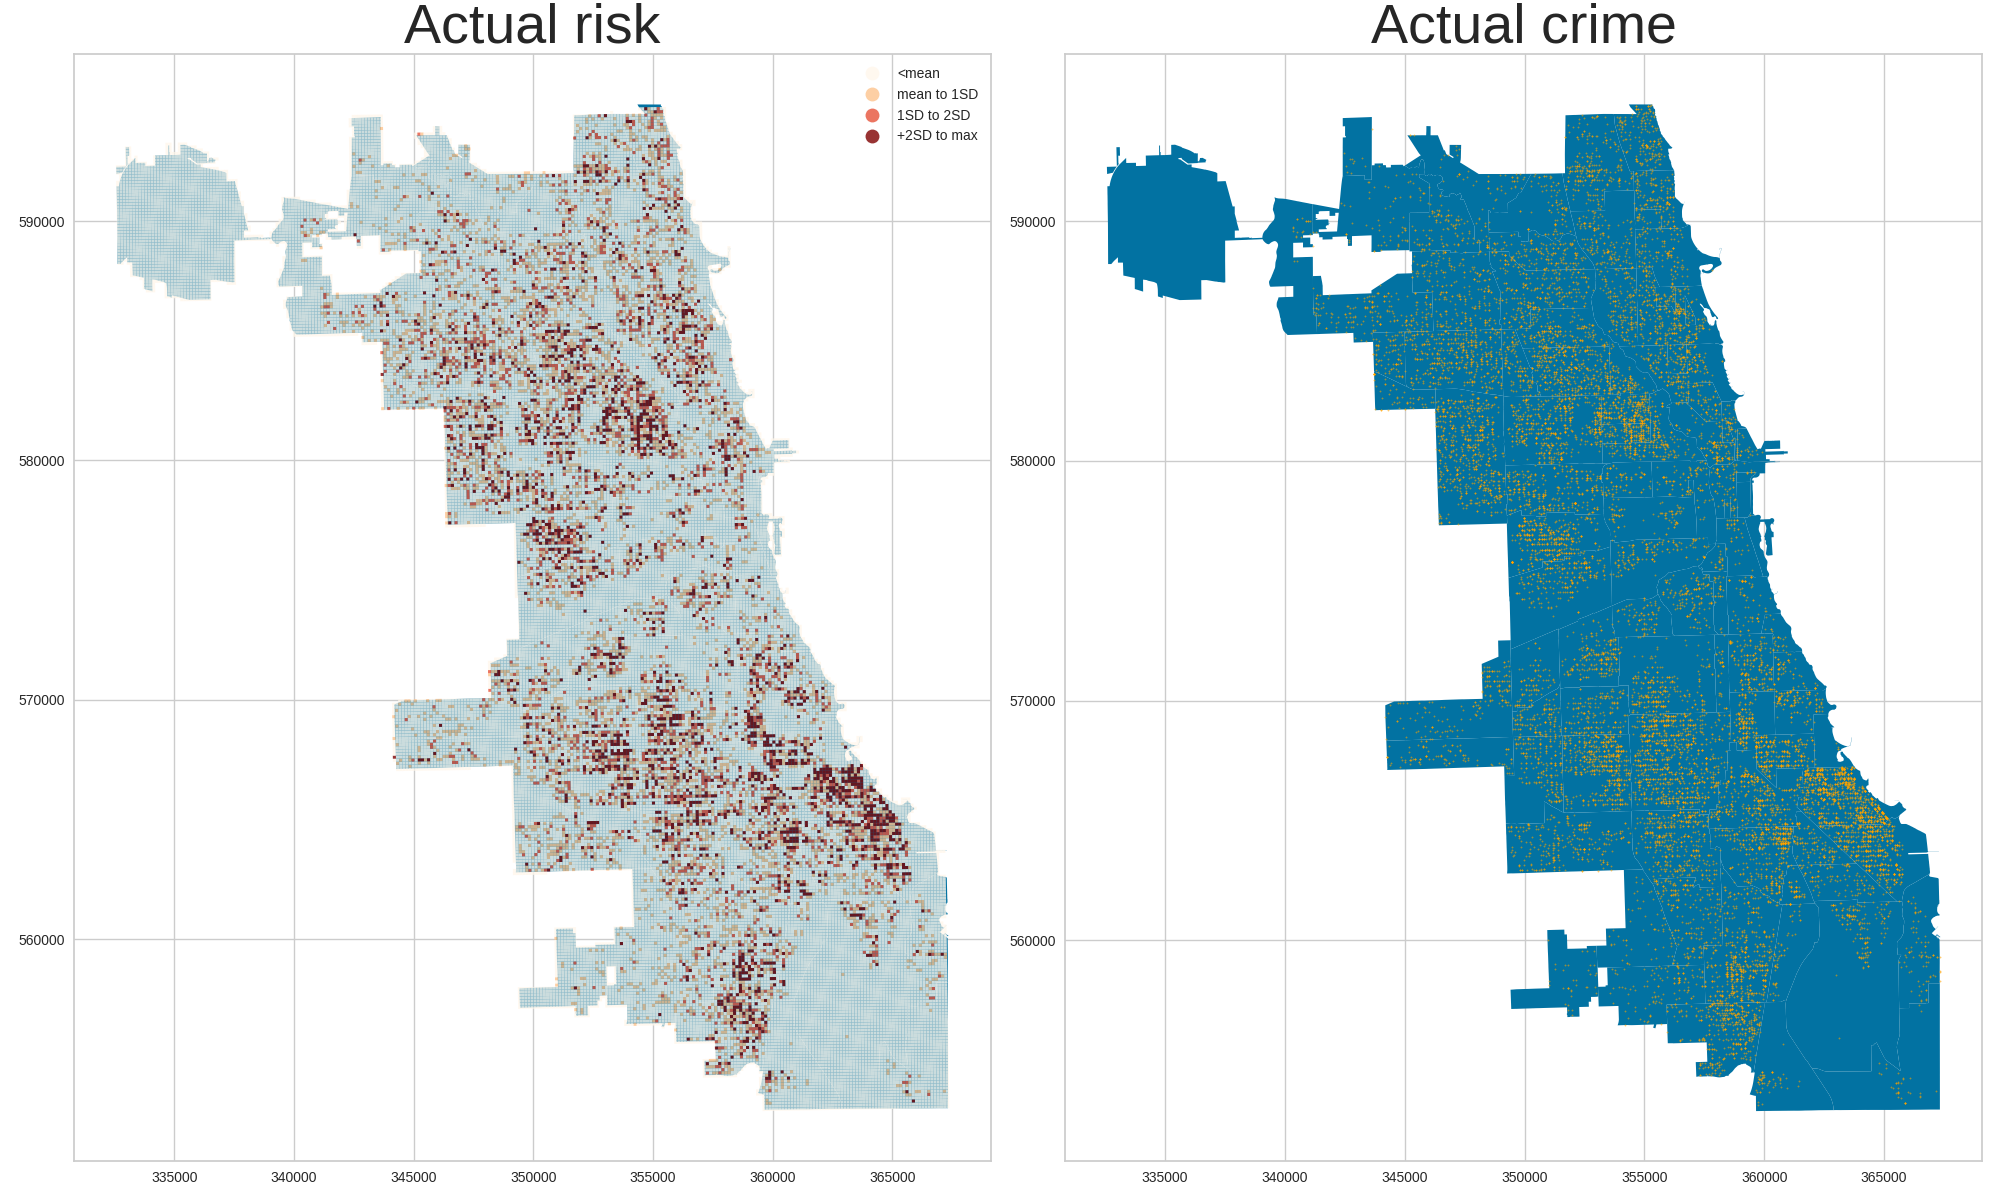
\includegraphics[scale=0.25]{./util-fig/actual_risk_point_map.png}
  \caption{左:実際のリスクマップ 右:実際の強盗犯罪発生地点}
  \label{fig:add-crime-timeseries-actual-risk}
\end{figure}

\begin{figure}
  \centering % 図を中央寄せにする
  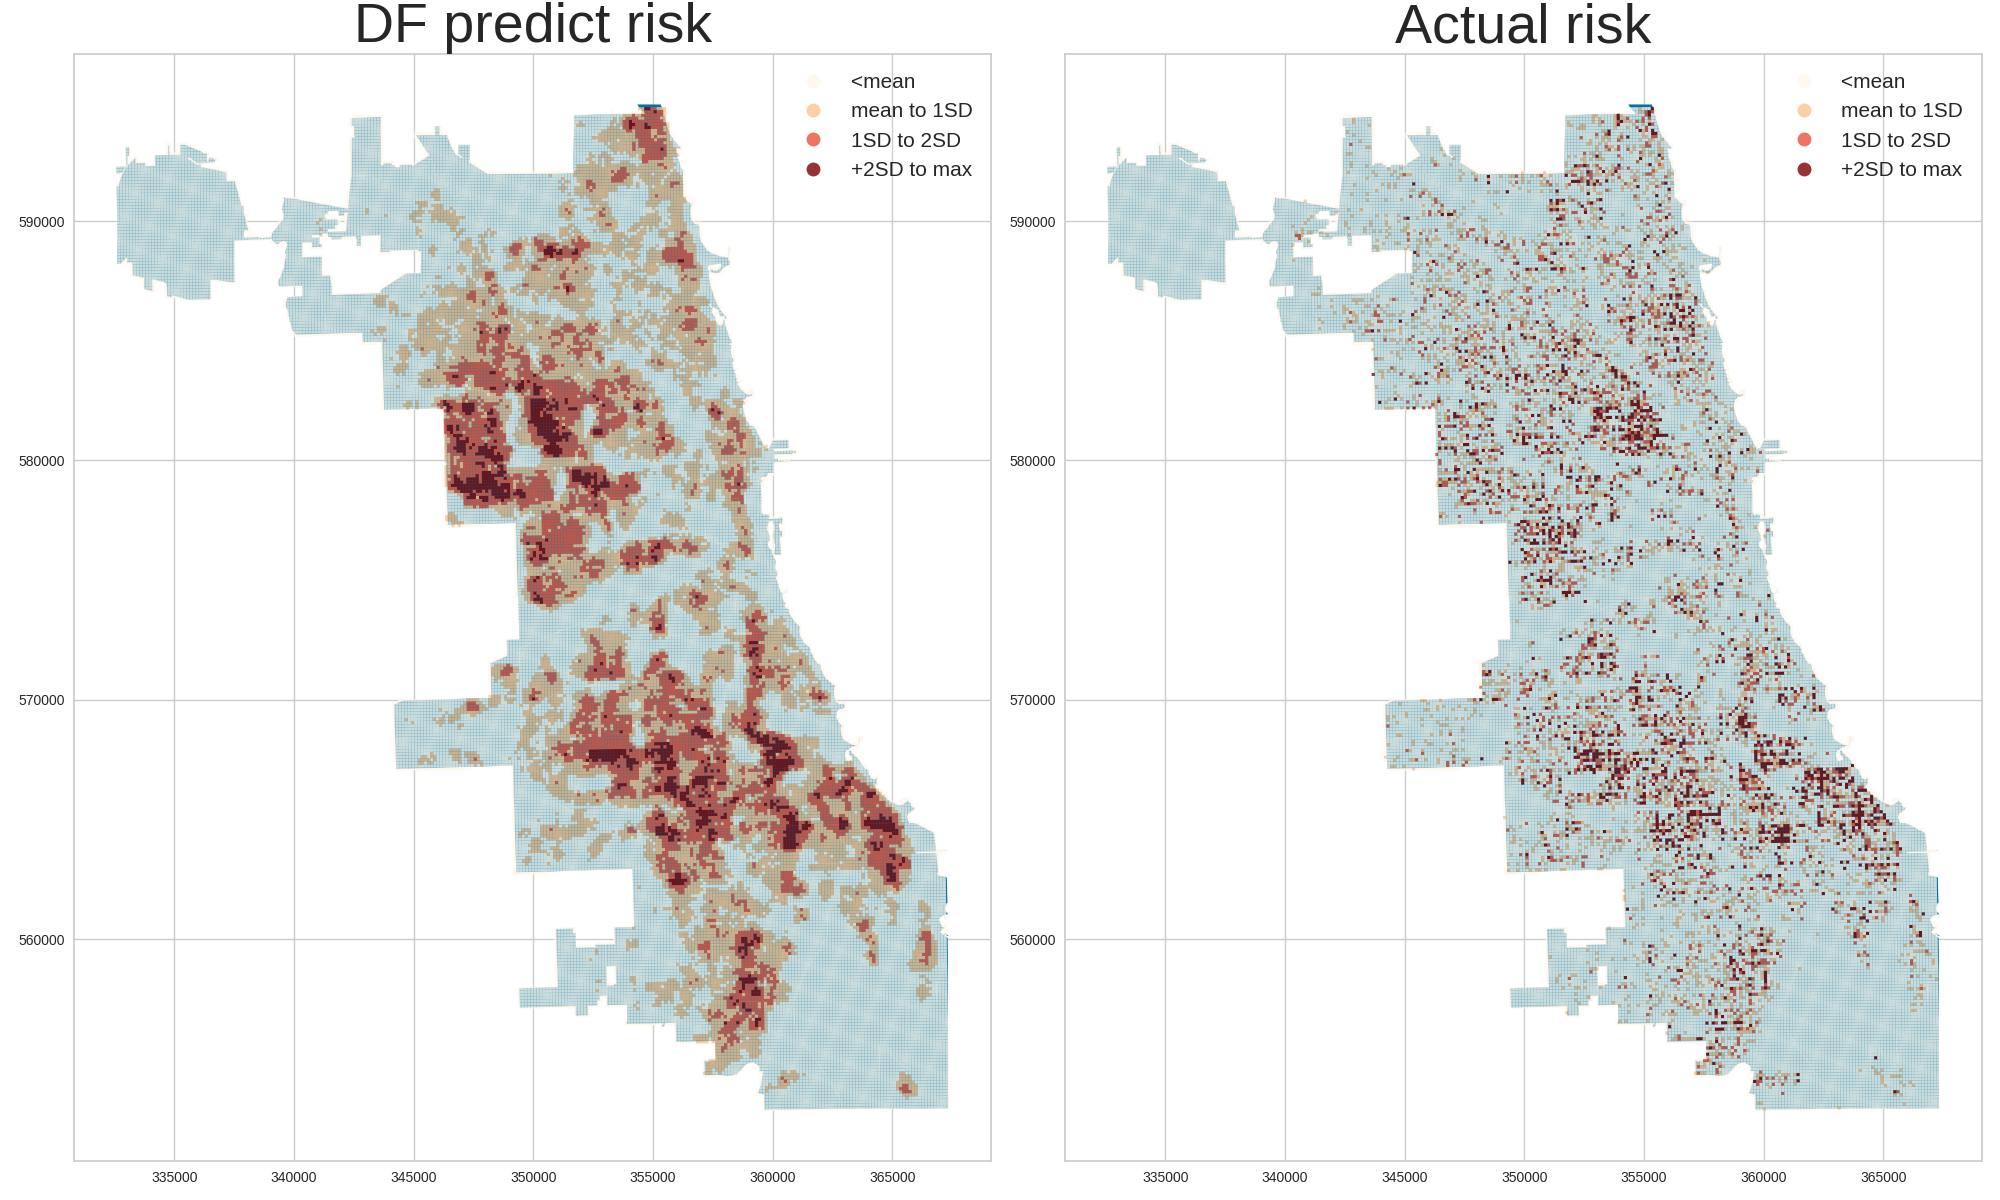
\includegraphics[scale=0.25]{./add-crime-timeseries-fig/DF_riskmap.png}
  \caption{左:DFによるリスクマップ 右:実際のリスクマップ}
  \label{fig:add-crime-timeseries-df-risk}
\end{figure}

\begin{figure}
  \centering % 図を中央寄せにする
  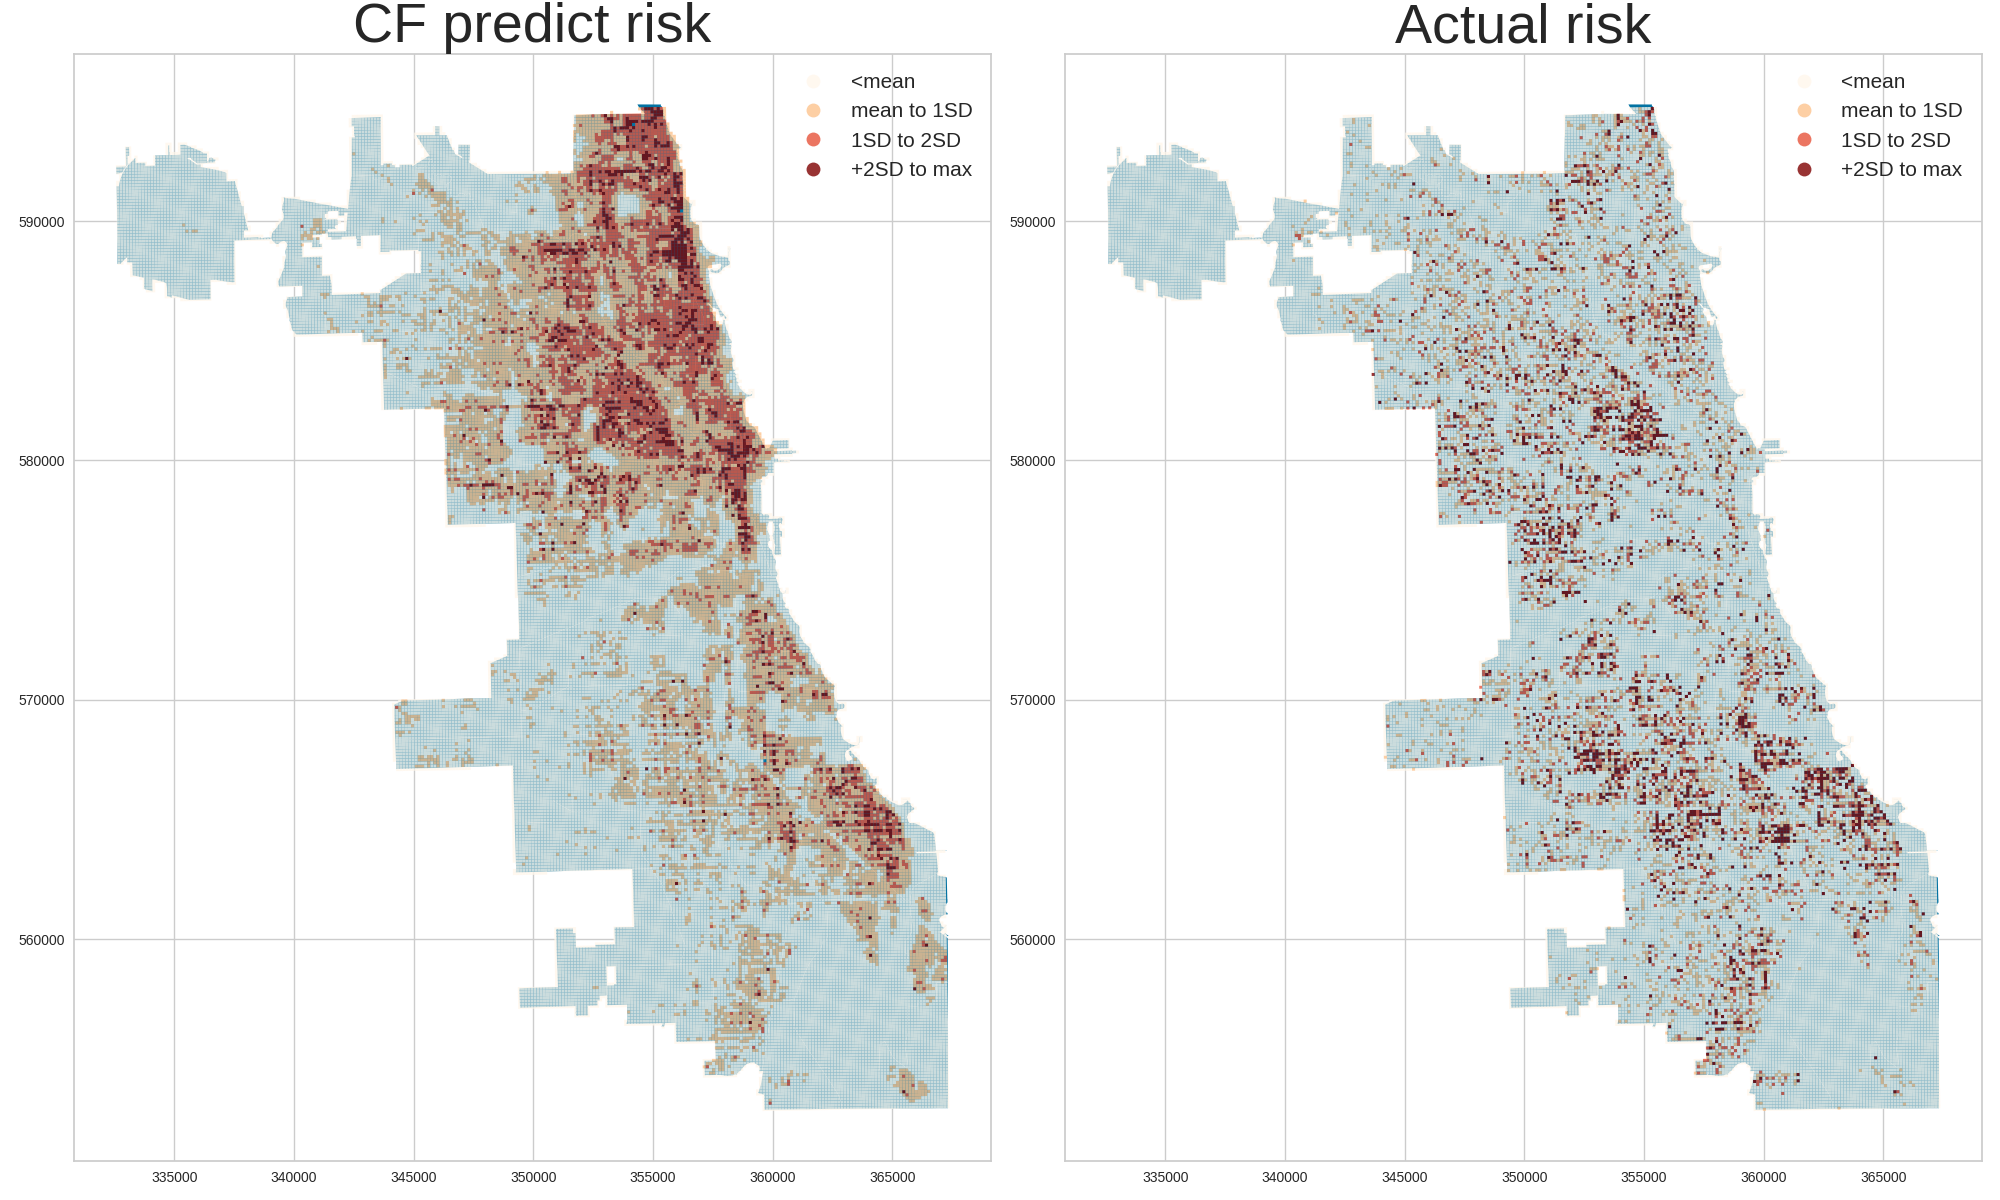
\includegraphics[scale=0.25]{./add-crime-timeseries-fig/CF_riskmap.png}
  \caption{左:CFによるリスクマップ 右:実際のリスクマップ}
  \label{fig:add-crime-timeseries-cf-risk}
\end{figure}

\begin{figure}
  \centering % 図を中央寄せにする
  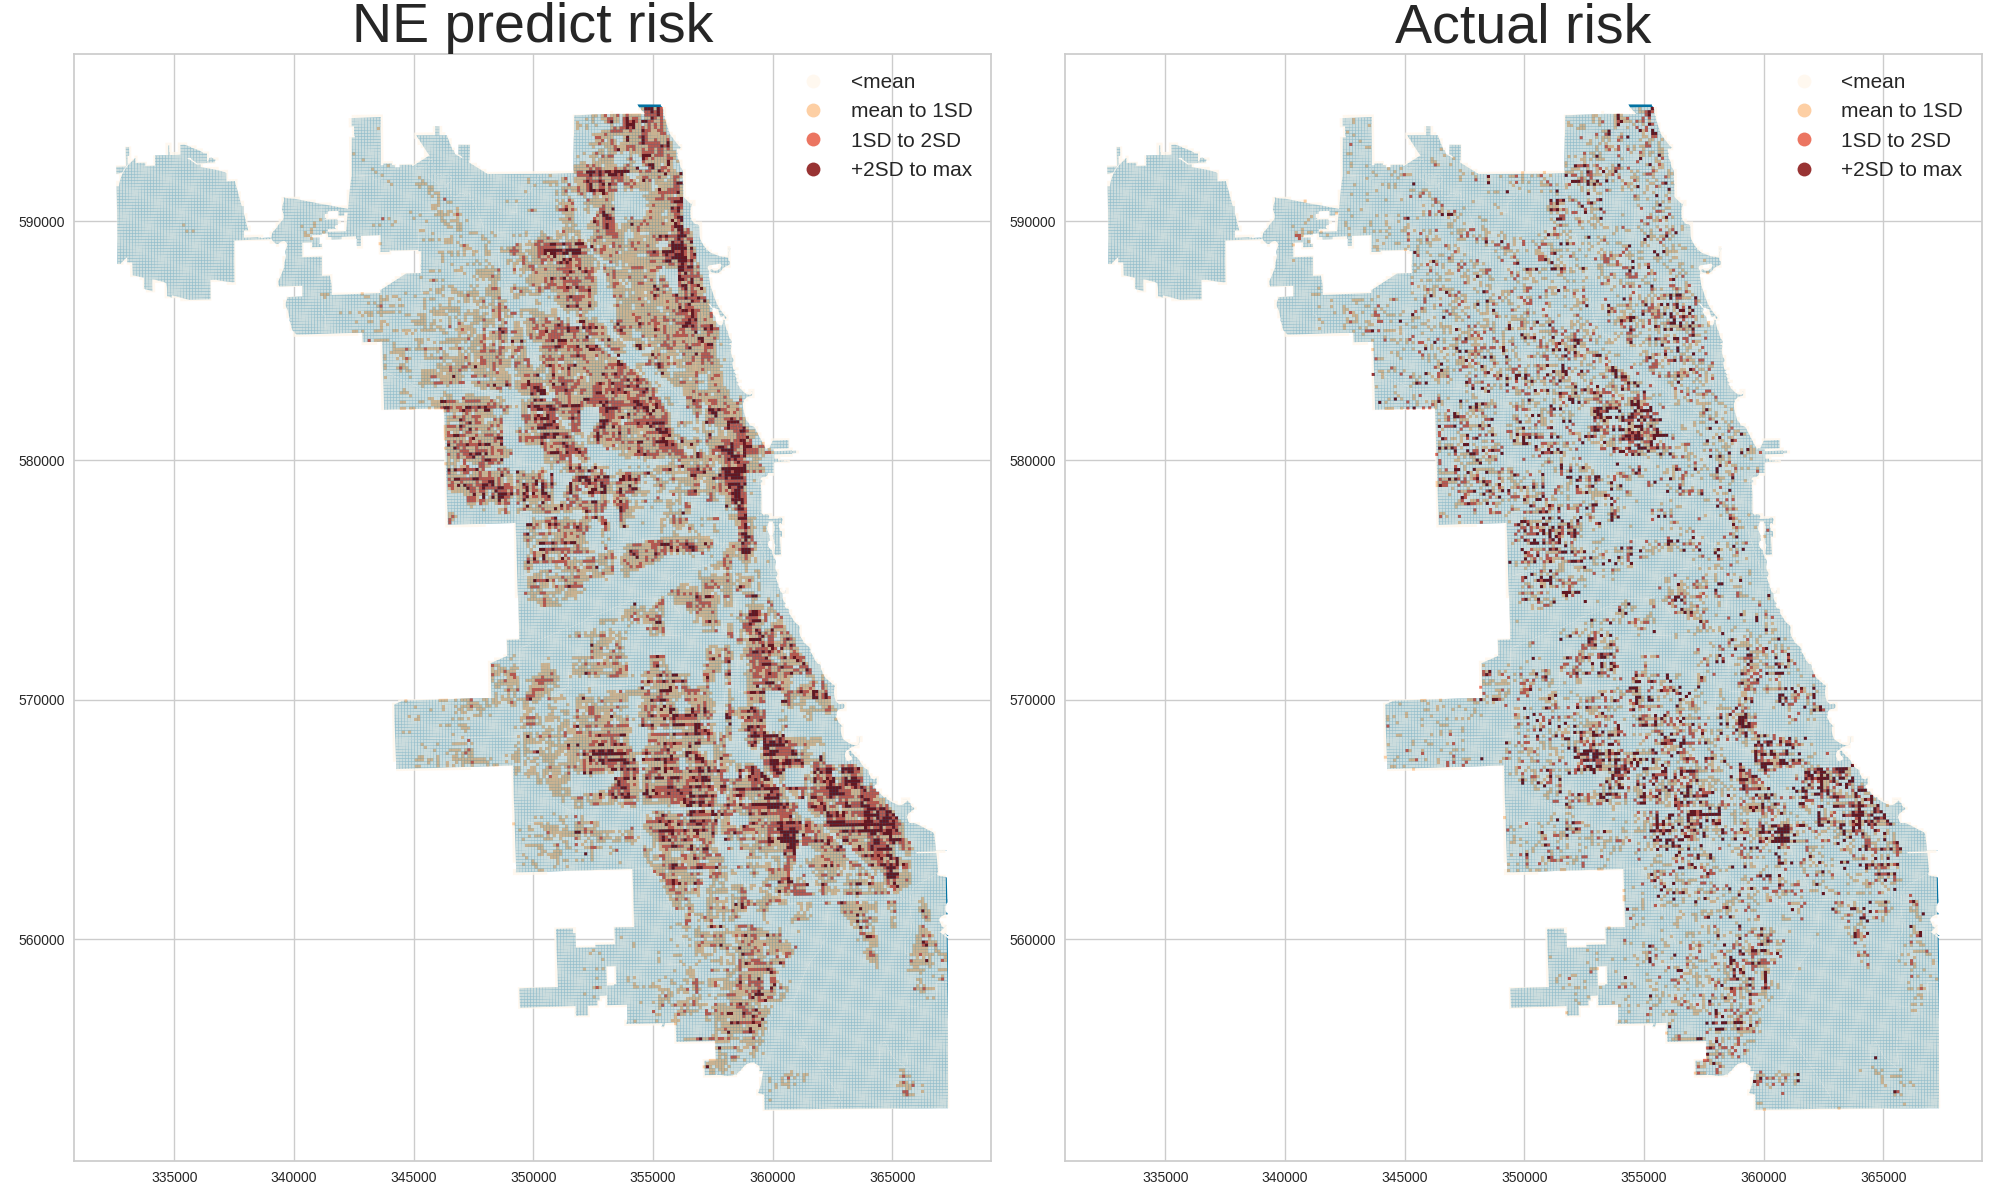
\includegraphics[scale=0.25]{./add-crime-timeseries-fig/NE_riskmap.png}
  \caption{左:NEによるリスクマップ 右:実際のリスクマップ}
  \label{fig:add-crime-timeseries-ne-risk}
\end{figure}

\begin{figure}
  \centering % 図を中央寄せにする
  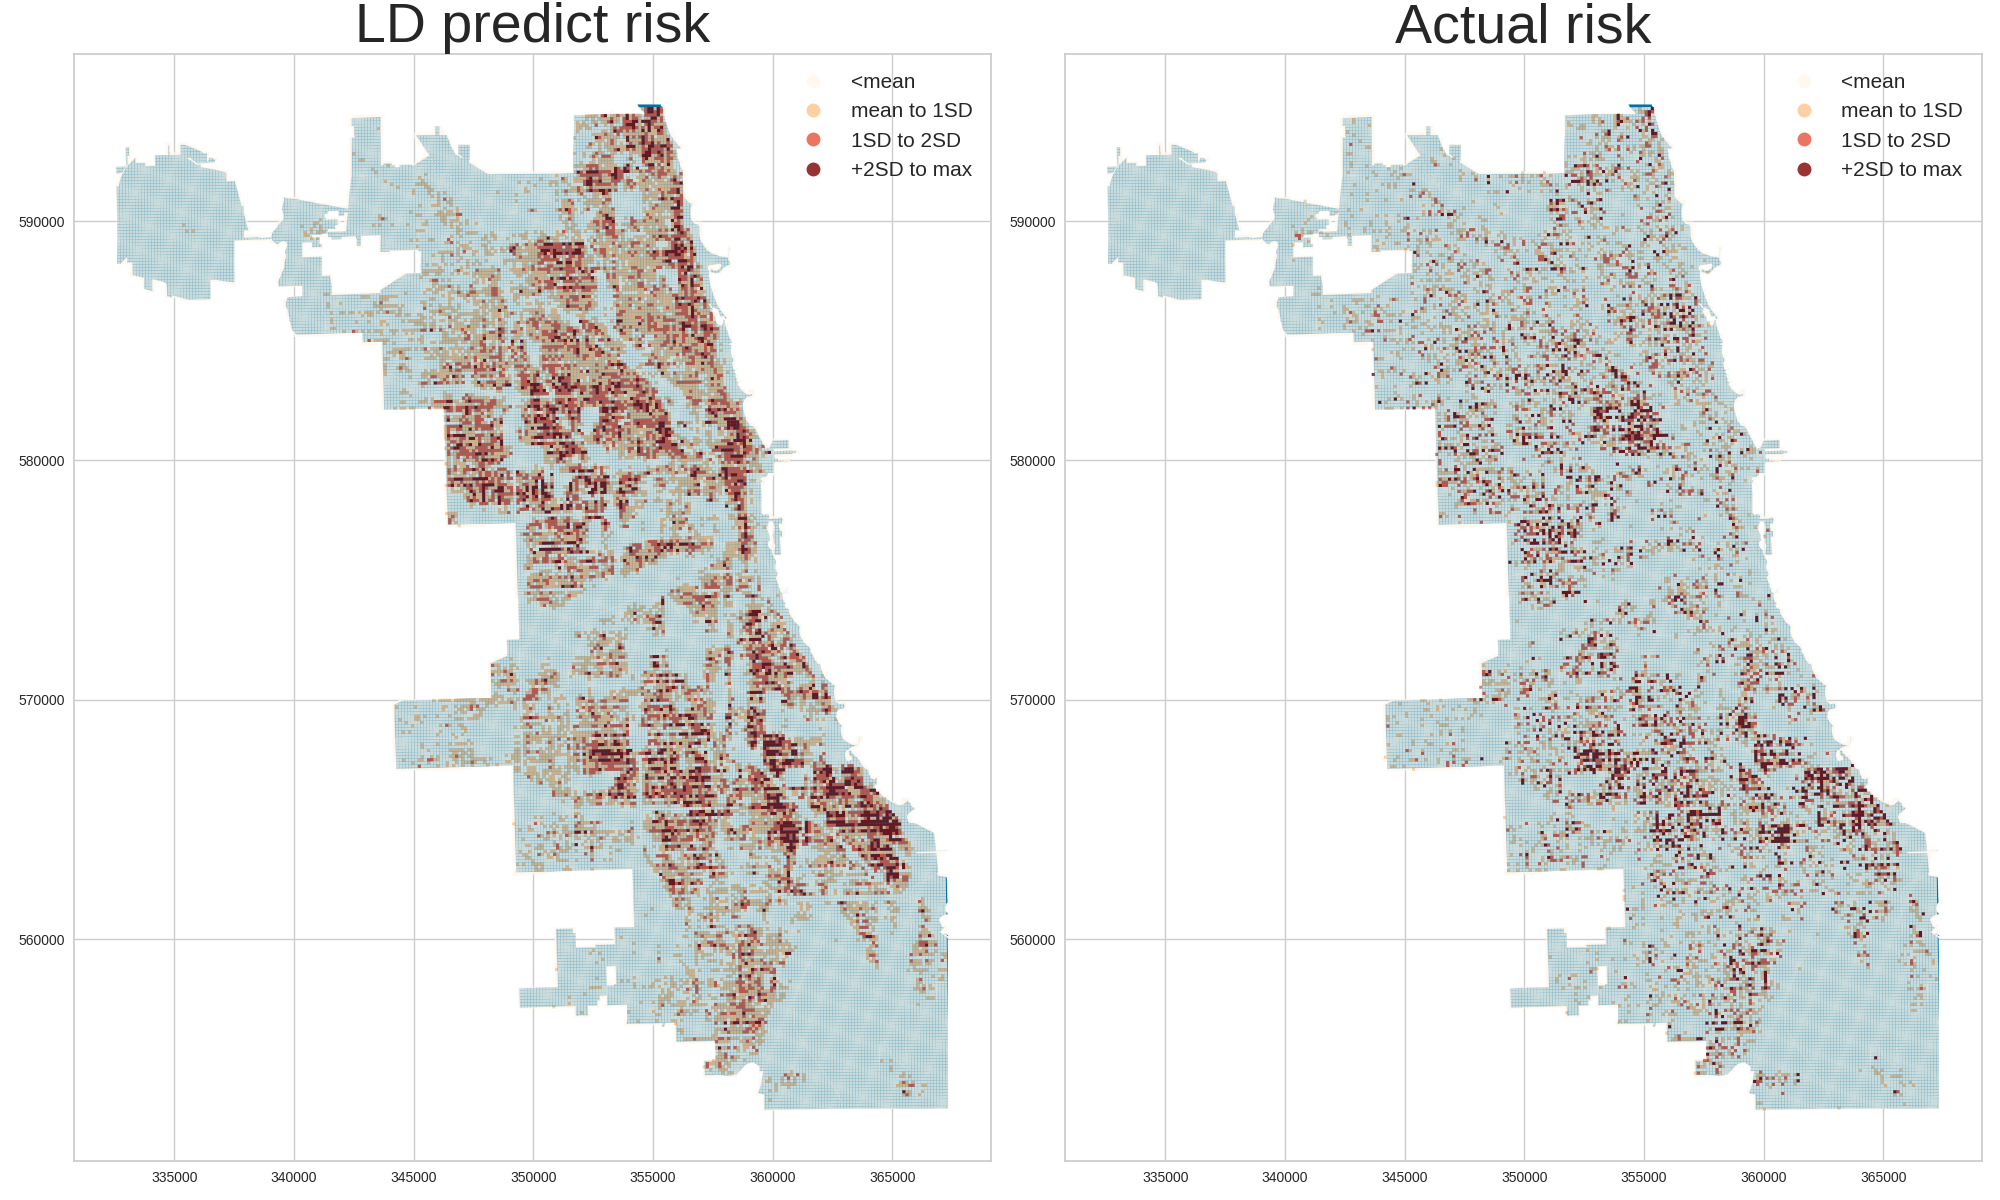
\includegraphics[scale=0.25]{./add-crime-timeseries-fig/LD_riskmap.png}
  \caption{左:LDによるリスクマップ 右:実際のリスクマップ}
  \label{fig:add-crime-timeseries-ld-risk}
\end{figure}

\begin{figure}
  \centering % 図を中央寄せにする
  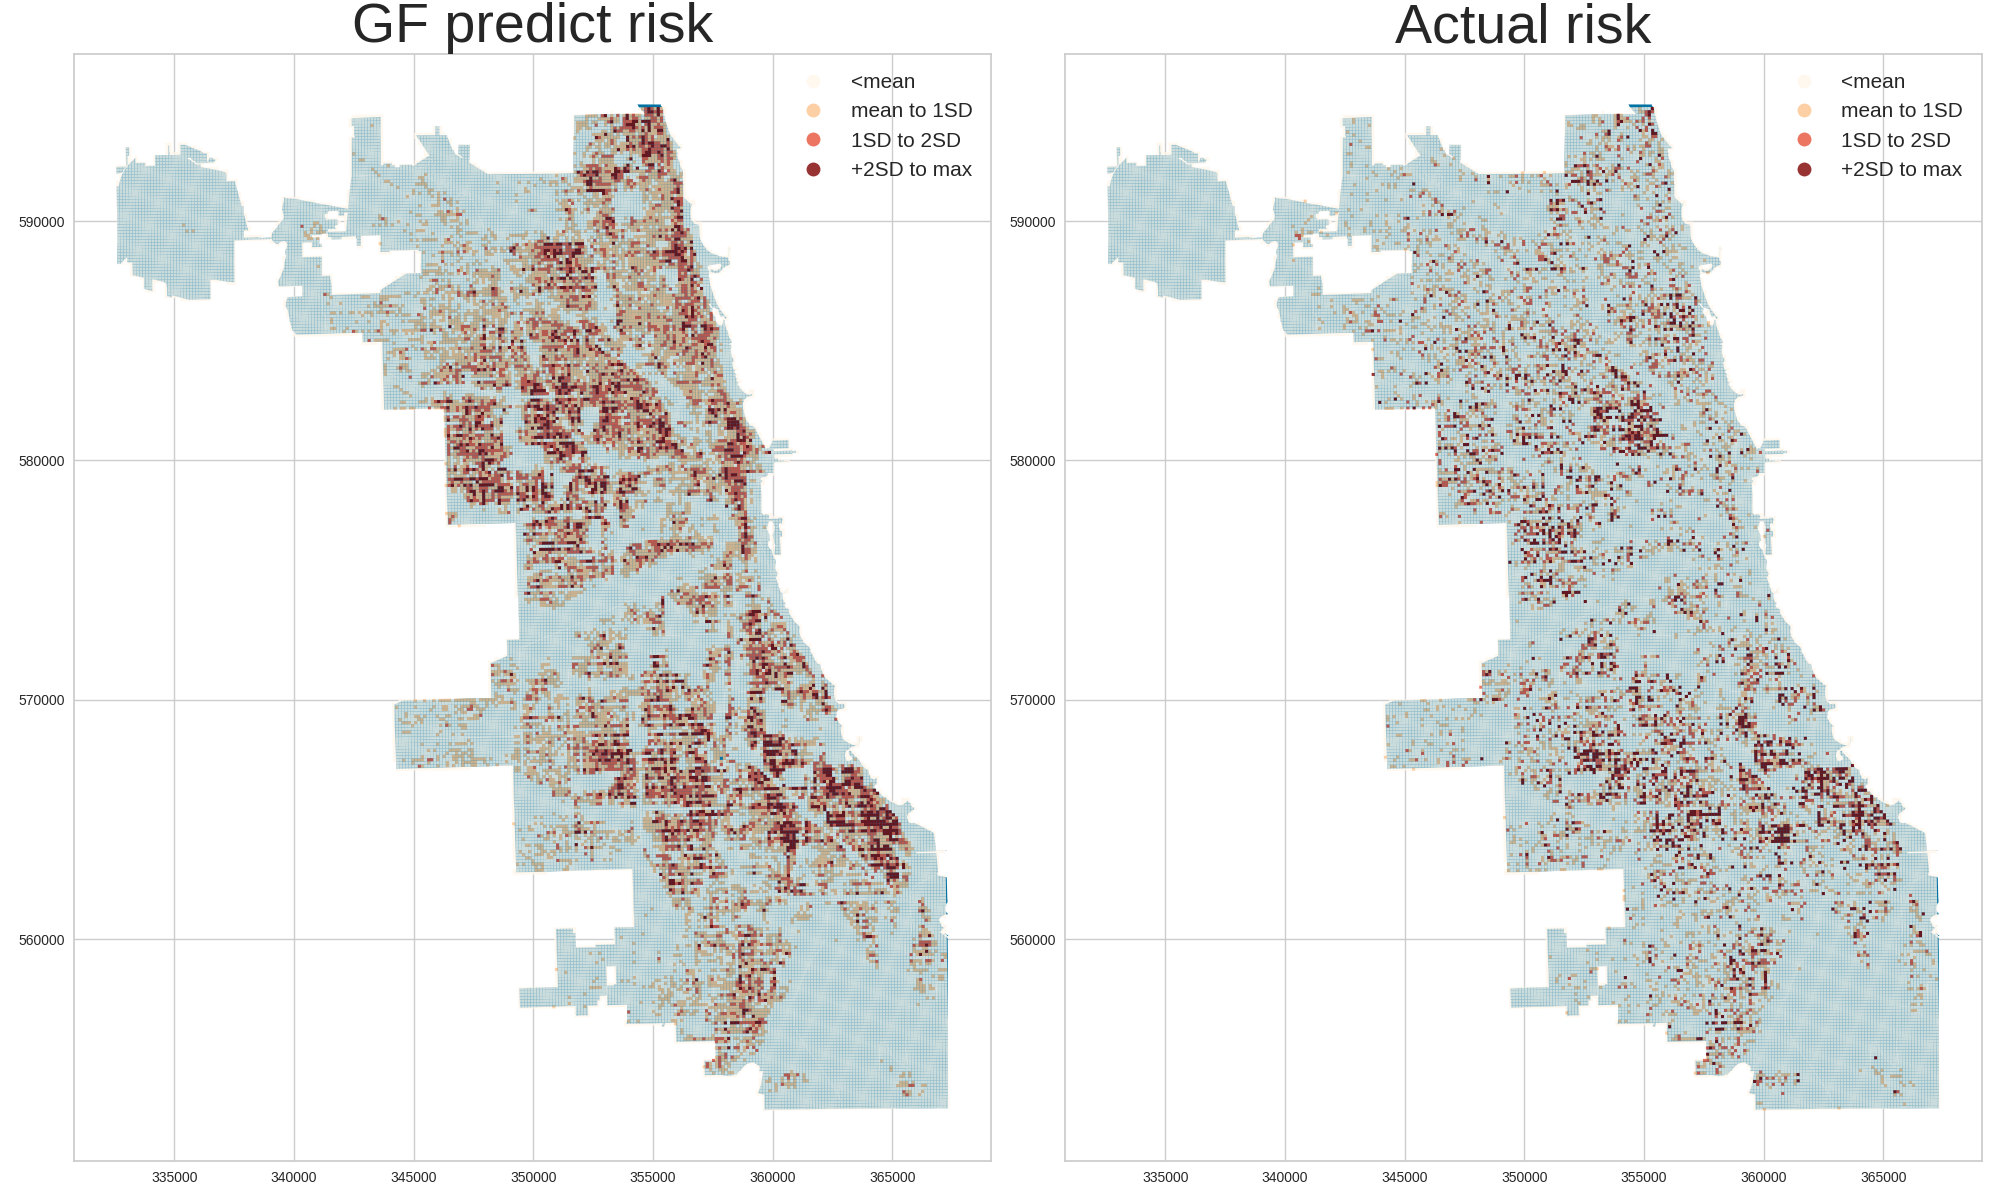
\includegraphics[scale=0.25]{./add-crime-timeseries-fig/GF_riskmap.png}
  \caption{左:GFによるリスクマップ 右:実際のリスクマップ}
  \label{fig:add-crime-timeseries-gf-risk}
\end{figure}

\begin{figure}
  \centering % 図を中央寄せにする
  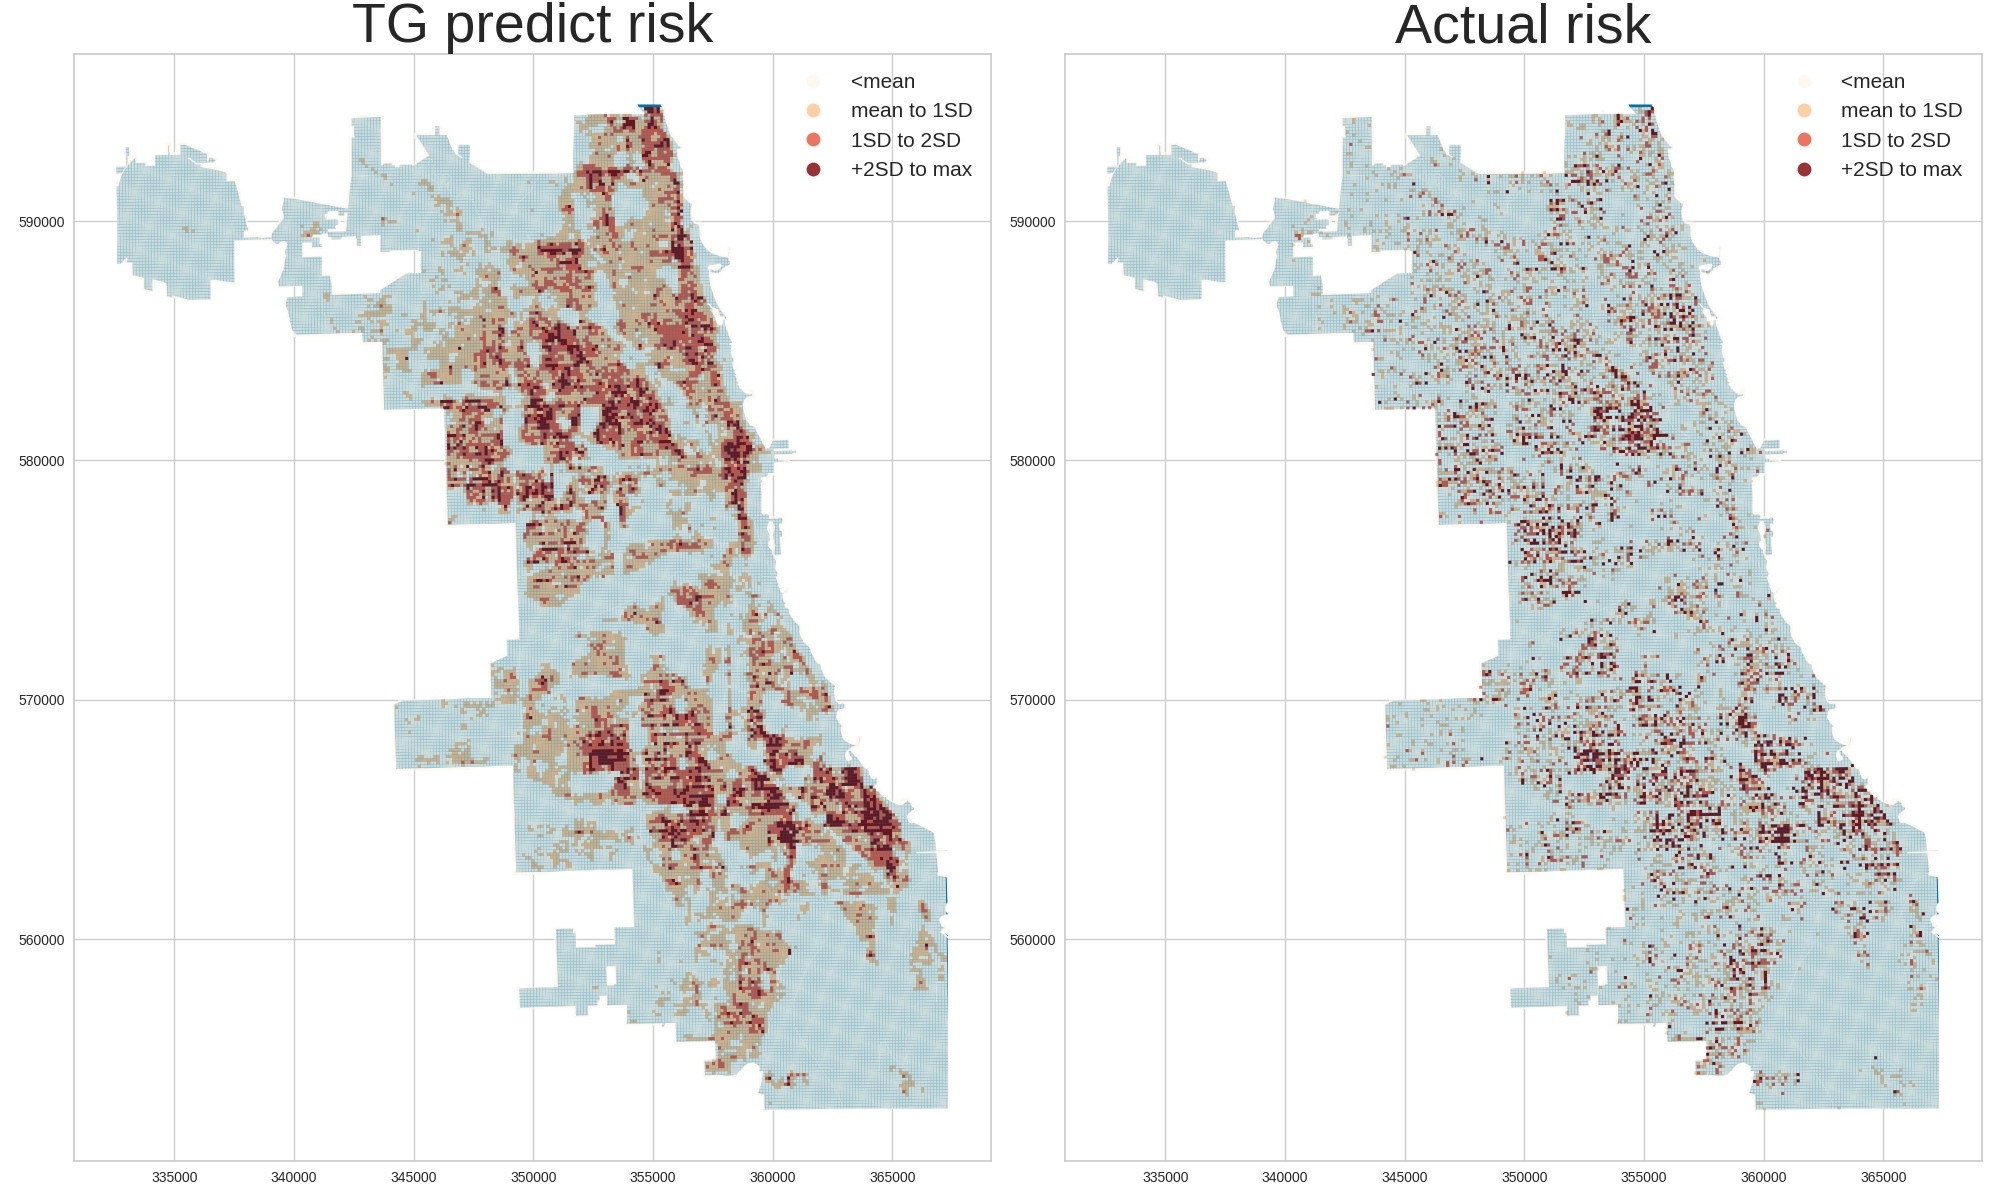
\includegraphics[scale=0.25]{./add-crime-timeseries-fig/TG_riskmap.png}
  \caption{左:TGによるリスクマップ 右:実際のリスクマップ}
  \label{fig:add-crime-timeseries-tg-risk}
\end{figure}

\begin{figure}
  \centering % 図を中央寄せにする
  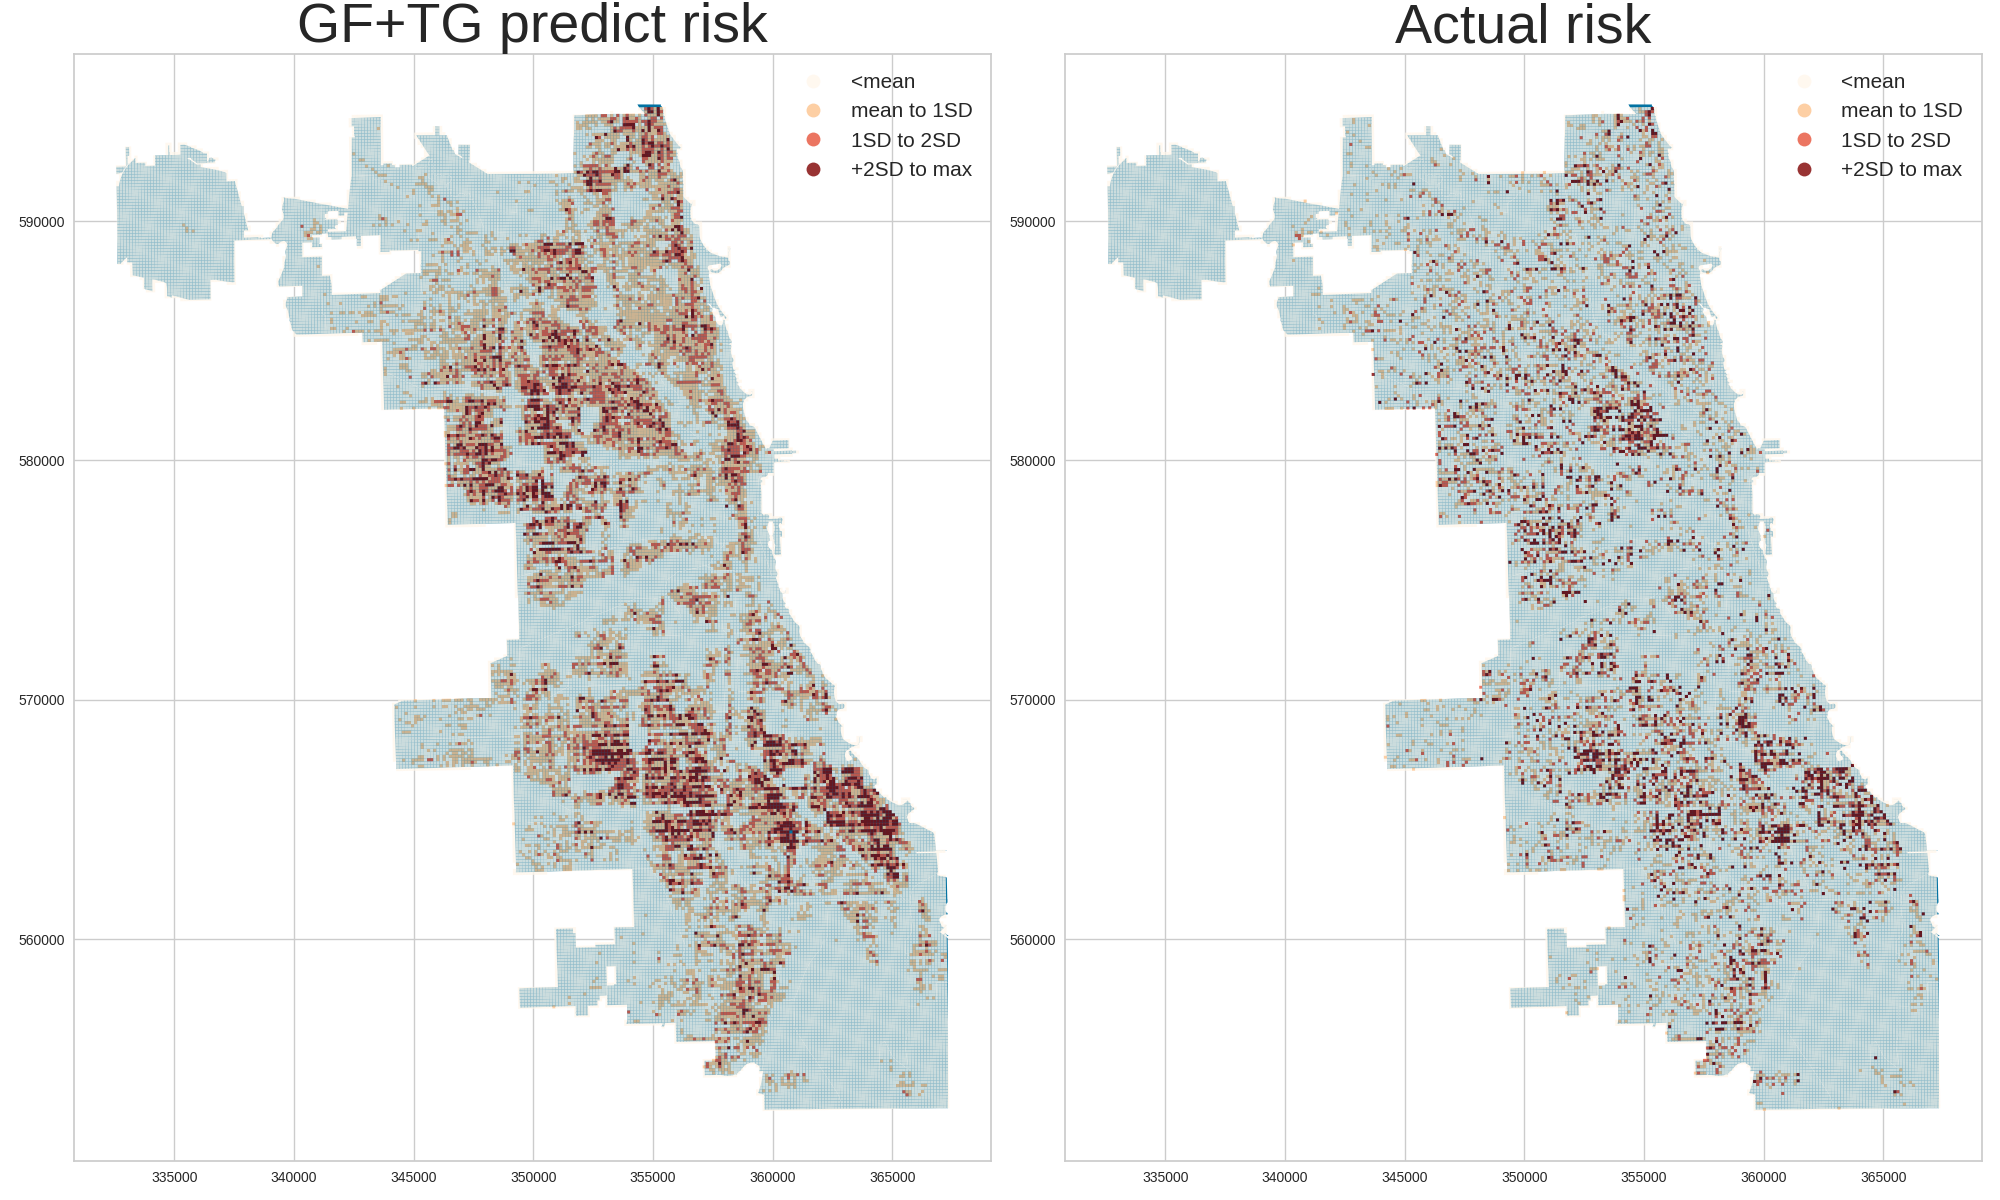
\includegraphics[scale=0.25]{./add-crime-timeseries-fig/GF+TG_riskmap.png}
  \caption{左:FG+TGによるリスクマップ 右:実際のリスクマップ}
  \label{fig:add-crime-timeseries-gf-tg-risk}
\end{figure}
%------------------------------------------
% confusion matrix
%------------------------------------------
\begin{figure}
  \centering % 図を中央寄せにする
  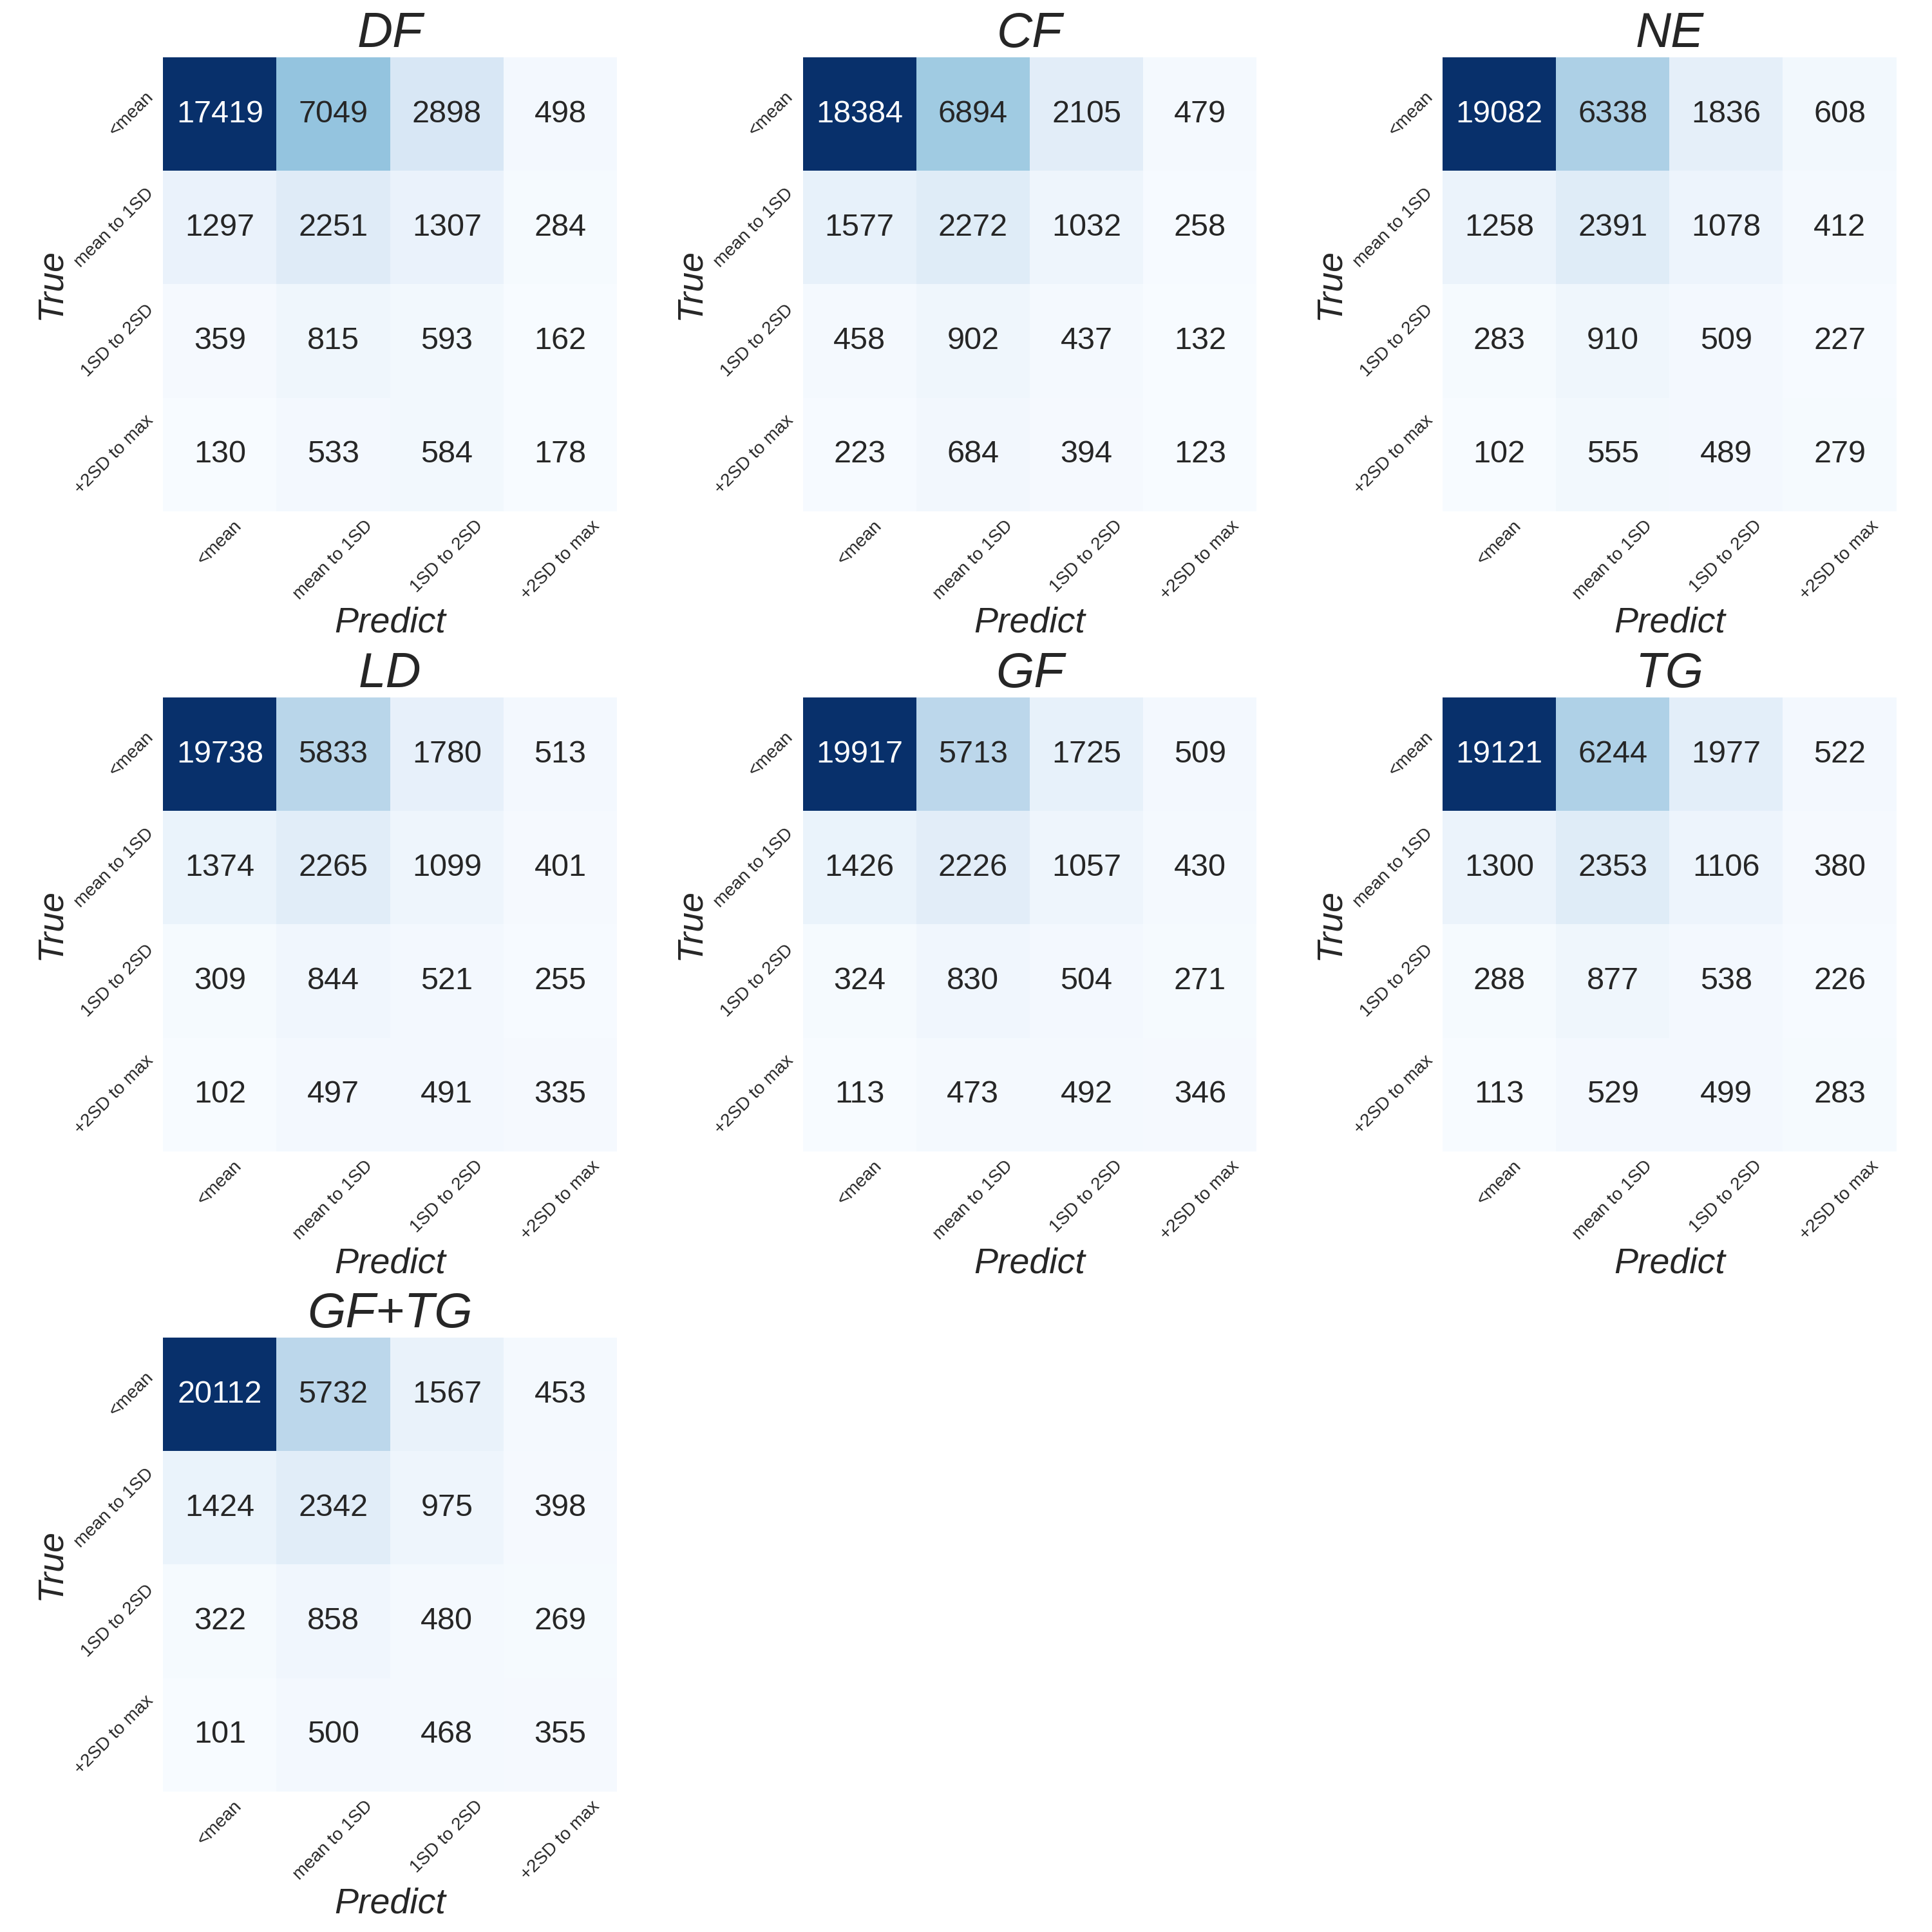
\includegraphics[scale=0.16]{./add-crime-timeseries-fig/non_crime_no_timeseries_four_cm.png}
  \caption{4カテゴリーの混同行列}
  \label{fig:add-crime-timeseries-4cm}
\end{figure}

\begin{figure}
  \centering % 図を中央寄せにする
  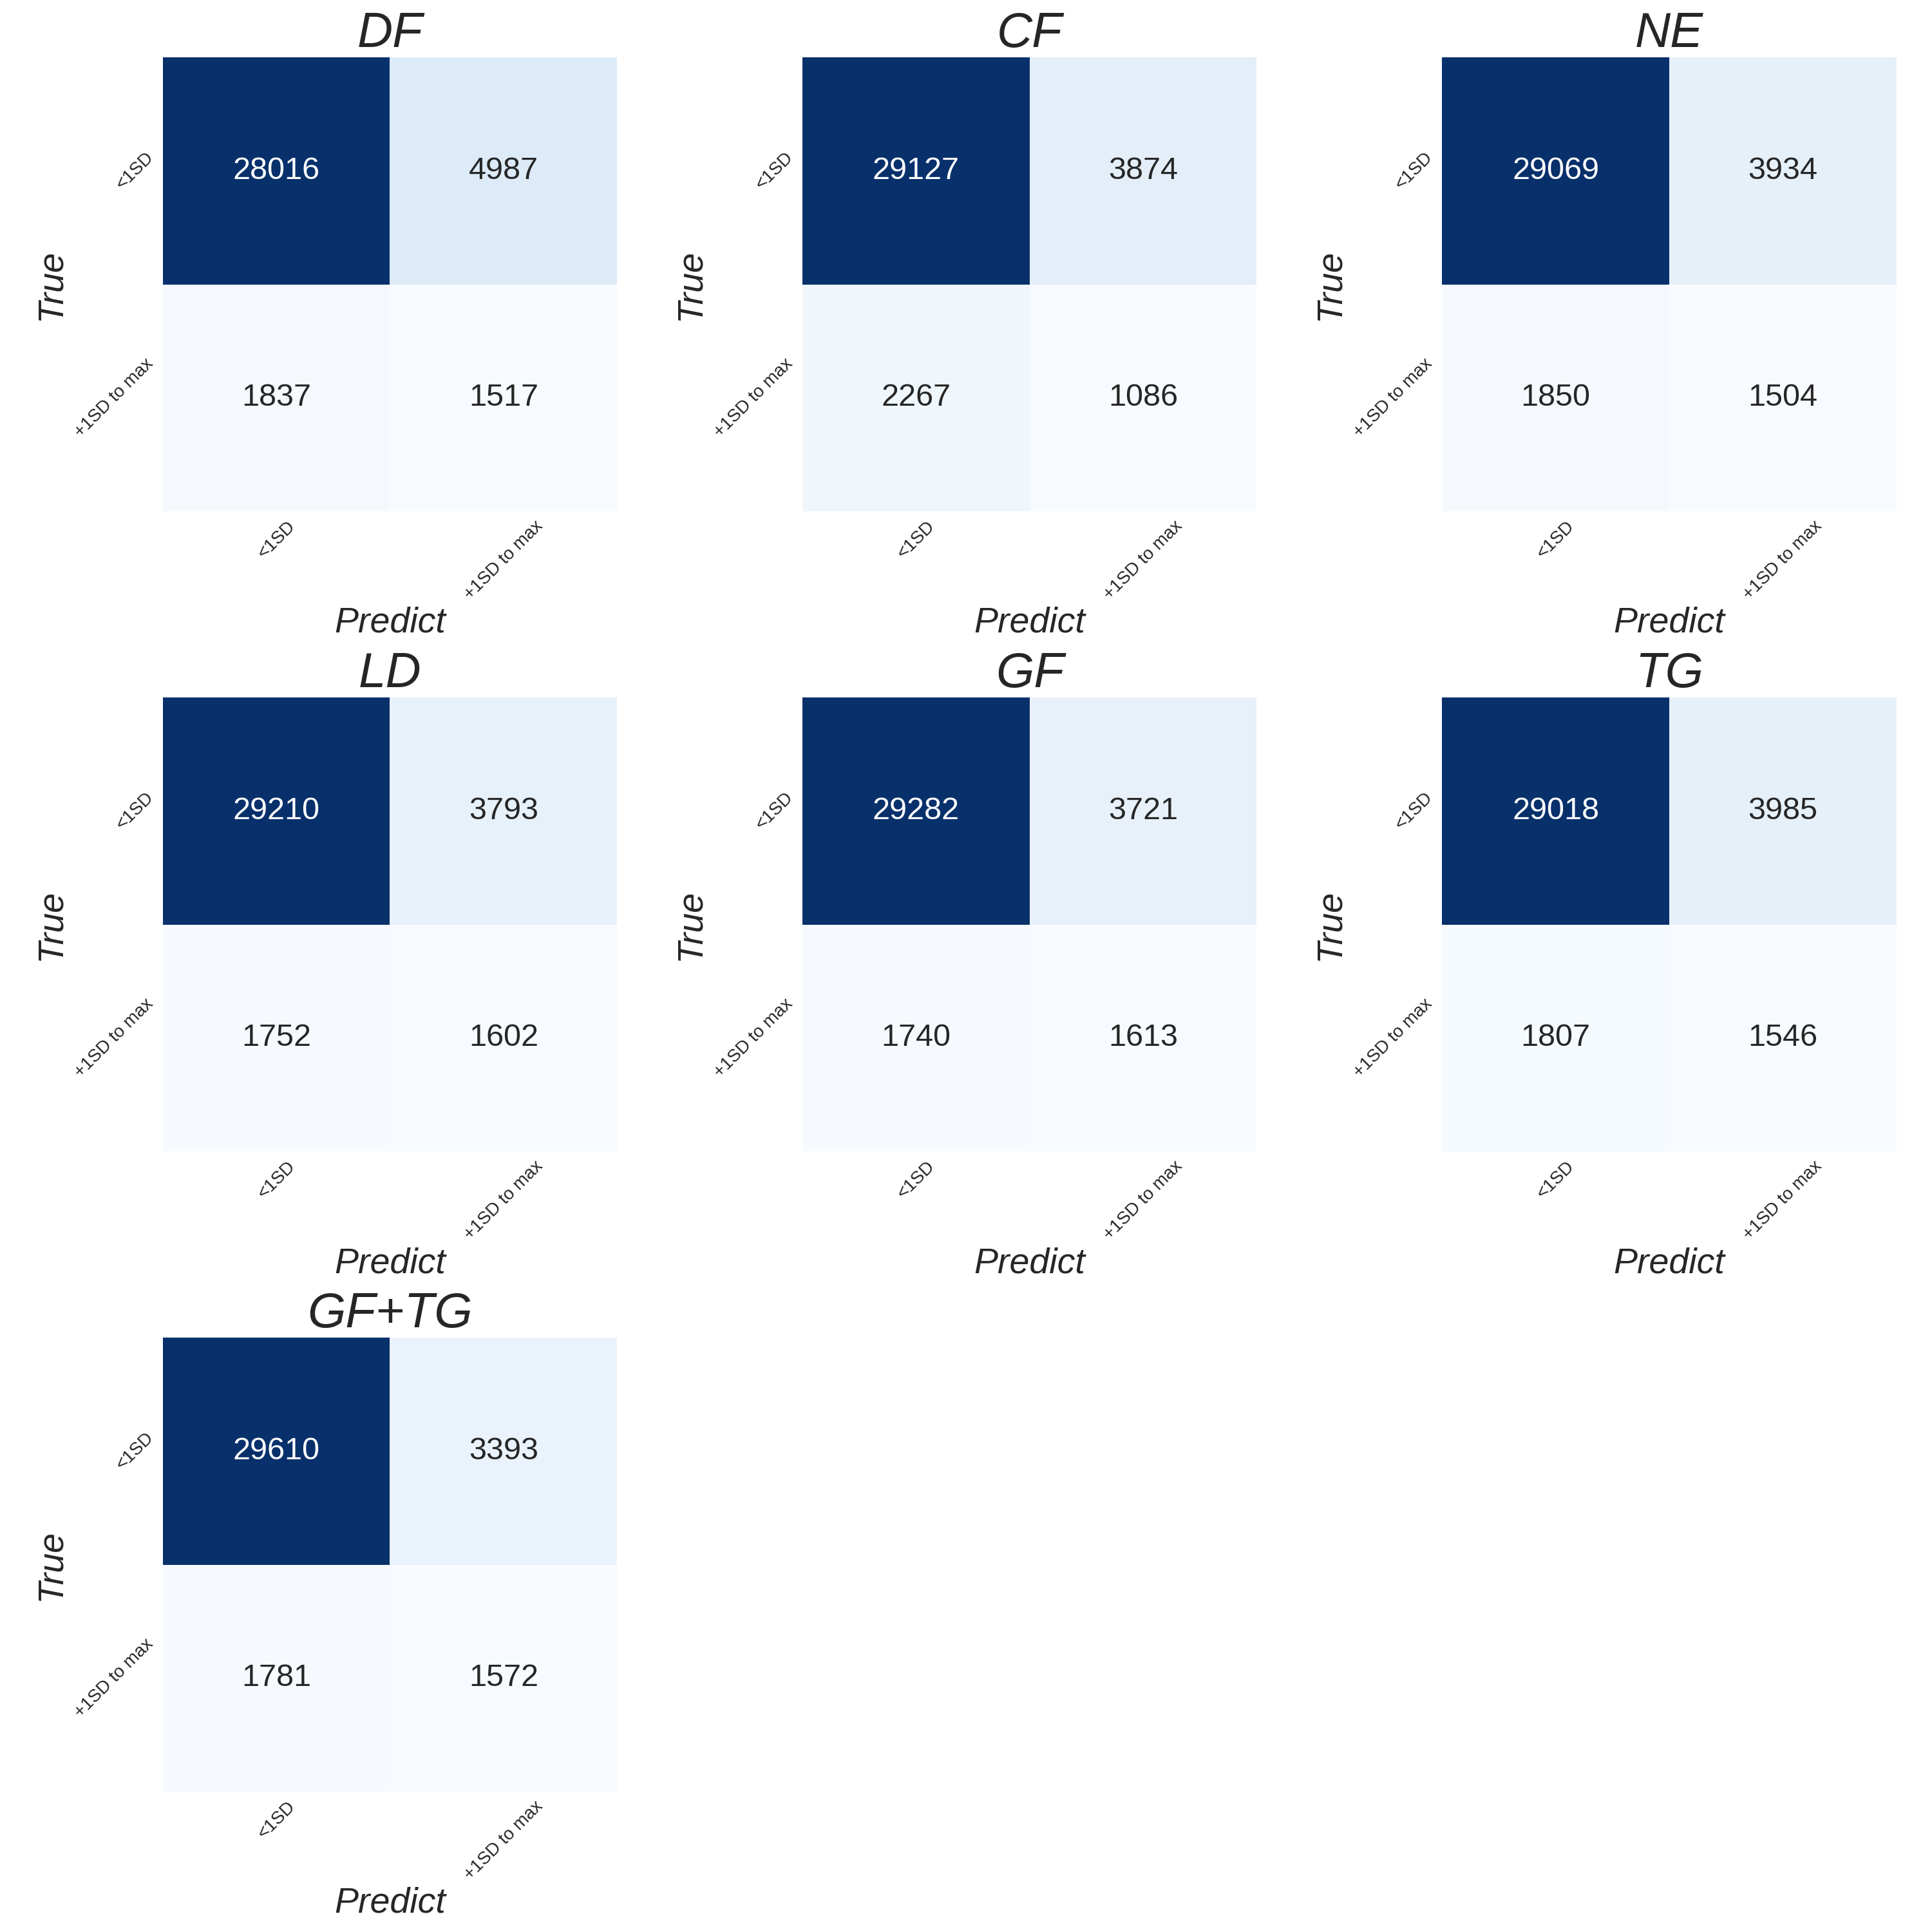
\includegraphics[scale=0.16]{./add-crime-timeseries-fig/non_crime_no_timeseries_two_cm.png}
  \caption{2カテゴリーの混同行列}
  \label{fig:add-crime-timeseries-2cm}
\end{figure}
% ---------------------------------
% FNFPplot
% ---------------------------------
\begin{figure}
  \centering % 図を中央寄せにする
  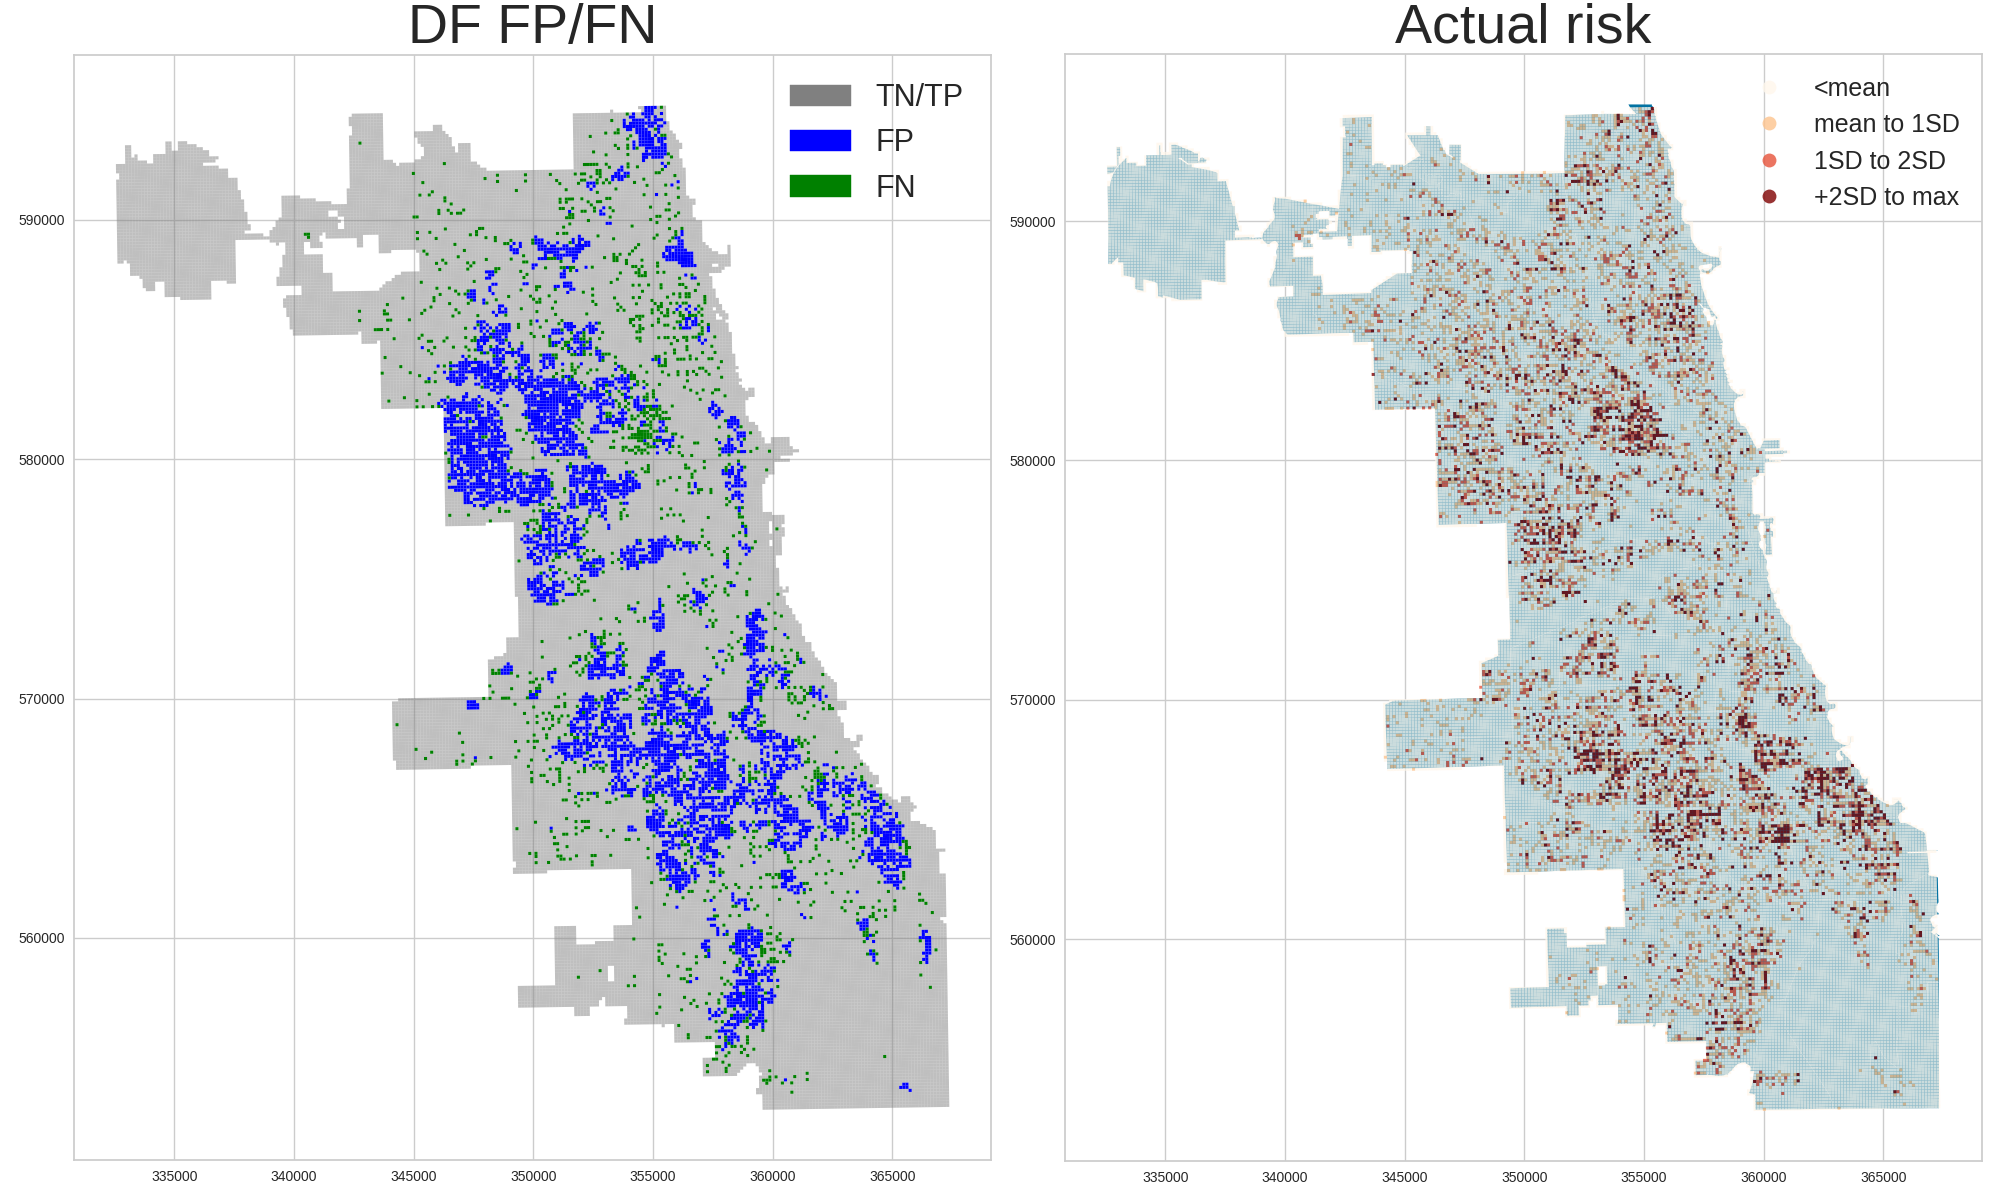
\includegraphics[scale=0.25]{./add-crime-timeseries-fig/DF_fnp.png}
  \caption{左:DFのFPFN 右:実際のリスクマップ}
  \label{fig:add-crime-timeseries-df-fnp}
\end{figure}

\begin{figure}
  \centering % 図を中央寄せにする
  \includegraphics[scale=0.25]{./add-crime-timeseries-fig/CF_fnp.png}
  \caption{左:CFのFPFN 右:実際のリスクマップ}
  \label{fig:add-crime-timeseries-cf-fnp}
\end{figure}

\begin{figure}
  \centering % 図を中央寄せにする
  \includegraphics[scale=0.25]{./add-crime-timeseries-fig/NE_fnp.png}
  \caption{左:NEのFPFN 右:実際のリスクマップ}
  \label{fig:add-crime-timeseries-ne-fnp}
\end{figure}

\begin{figure}
  \centering % 図を中央寄せにする
  \includegraphics[scale=0.25]{./add-crime-timeseries-fig/LD_fnp.png}
  \caption{左:LDのFPFN 右:実際のリスクマップ}
  \label{fig:add-crime-timeseries-ld-fnp}
\end{figure}

\begin{figure}
  \centering % 図を中央寄せにする
  \includegraphics[scale=0.25]{./add-crime-timeseries-fig/GF_fnp.png}
  \caption{左:GFのFPFN 右:実際のリスクマップ}
  \label{fig:add-crime-timeseries-gf-fnp}
\end{figure}

\begin{figure}
  \centering % 図を中央寄せにする
  \includegraphics[scale=0.25]{./add-crime-timeseries-fig/TG_fnp.png}
  \caption{左:TGのFPFN 右:実際のリスクマップ}
  \label{fig:add-crime-timeseries-tg-fnp}
\end{figure}

\begin{figure}
  \centering % 図を中央寄せにする
  \includegraphics[scale=0.25]{./add-crime-timeseries-fig/GF+TG_fnp.png}
  \caption{左:GF+TGのFPFN 右:実際のリスクマップ}
  \label{fig:add-crime-timeseries-gf-tg-fnp}
\end{figure}
%------------------------------------------
% ROC curve
%------------------------------------------
また,各モデルのROC曲線を図\ref{fig:add-crime-timeseries-roc}に示した.

\begin{figure}
  \centering % 図を中央寄せにする
  \includegraphics[scale=0.25]{./add-crime-timeseries-fig/roc_auc.png}
  \caption{ROC曲線}
  \label{fig:add-crime-timeseries-roc}
\end{figure}
%------------------------------------------
% table
%------------------------------------------
各モデルの予測精度を精度指標を基に比較した結果を表\ref{tb:fig:add-crime-timeseries-index}にまとめる.

\begin{table}[htbp]
  \centering
  \caption{各モデル間の精度比較}
  \begin{tabular}{l|r|r|r|r|r|r|r}
  \hline

  モデル & DF & CF & NE & LD & GF & TG & GF+TG \\  \hline\hline
  的中率 & 42.6 & 31.3 & 41.9 & 44.3 & 44.6 & 42.5 & 42.9 \\ 
  PAI & 2.38 & 2.29 & 2.80 & 2.99 & 3.04 & 2.79 & 3.14 \\ 
  AUC & 0.78 & 0.76 & 0.82 & 0.83 & 0.83 & 0.82 & 0.84 \\ \hline
  


  \end{tabular}
  \label{tb:fig:add-crime-timeseries-index}
\end{table}

\FloatBarrier
%------------------------------------
%   Chapter 5
\chapter{おわりに}
% \label{chapter_5}
%------------------------------------
これまでに書いた内容を簡潔にまとめる。
ただし,第1章とは異なり,
ここまで論文を読み終えた読者を想定しているため,
これまでに登場した専門用語や事実等を
改めて説明することなく使用してかまわない。
「~を考察した。」ではなく,
「~であることが分かった。」のように
結論を述べる。
今後の課題も書く。


%------------------------------------
%   Acknowledgements
\chapter*{謝辞}
%------------------------------------
\addcontentsline{toc}{chapter}{謝辞}
(研究を遂行するにあたってサポートしてくれた方々へ
謝辞を述べるコーナー。
名前だけでなくどのようなサポートをしてくれたのかも書く。)

(例)
本研究を進めるにあたりご指導頂きました
鈴木一弘先生に感謝いたします。
本論文で主査と副査をして頂きました
\CID{8705}田直樹先生と塩田研一先生に感謝いたします。
日頃の議論を通じて多くの知識や示唆を頂きました
鈴木研究室の皆様に感謝いたします。



%------------------------------------
%   References
%------------------------------------
\bibliography{main} %hoge.bibから拡張子を外した名前
\bibliographystyle{plainnat} %参考文献出力スタイル
%------------------------------------
\appendix
%------------------------------------
\chapter{プログラム}
\label{program}
% \inputminted[breaklines,breakanywhere,linenos,tabsize=4]
% {JavaScript}{discrete_geometry.js}


%------------------------------------
\end{document}
%------------------------------------
